\PassOptionsToPackage{unicode=true}{hyperref} % options for packages loaded elsewhere
\PassOptionsToPackage{hyphens}{url}
%
\documentclass[12pt,]{article}
\usepackage{lmodern}
\usepackage{amssymb,amsmath}
\usepackage{ifxetex,ifluatex}
\usepackage{fixltx2e} % provides \textsubscript
\ifnum 0\ifxetex 1\fi\ifluatex 1\fi=0 % if pdftex
  \usepackage[T1]{fontenc}
  \usepackage[utf8]{inputenc}
  \usepackage{textcomp} % provides euro and other symbols
\else % if luatex or xelatex
  \usepackage{unicode-math}
  \defaultfontfeatures{Ligatures=TeX,Scale=MatchLowercase}
\fi
% use upquote if available, for straight quotes in verbatim environments
\IfFileExists{upquote.sty}{\usepackage{upquote}}{}
% use microtype if available
\IfFileExists{microtype.sty}{%
\usepackage[]{microtype}
\UseMicrotypeSet[protrusion]{basicmath} % disable protrusion for tt fonts
}{}
\IfFileExists{parskip.sty}{%
\usepackage{parskip}
}{% else
\setlength{\parindent}{0pt}
\setlength{\parskip}{6pt plus 2pt minus 1pt}
}
\usepackage{hyperref}
\hypersetup{
            pdftitle={Deliberative Bayesianism: Abduction, Reflection, and the Weight of Evidence},
            pdfauthor={Lok C. Chan},
            pdfborder={0 0 0},
            breaklinks=true}
\urlstyle{same}  % don't use monospace font for urls
\usepackage[left=1.5in,right=1in,top=1.5in,bottom=1.5in]{geometry}
\usepackage{longtable,booktabs}
% Fix footnotes in tables (requires footnote package)
\IfFileExists{footnote.sty}{\usepackage{footnote}\makesavenoteenv{longtable}}{}
\usepackage{graphicx,grffile}
\makeatletter
\def\maxwidth{\ifdim\Gin@nat@width>\linewidth\linewidth\else\Gin@nat@width\fi}
\def\maxheight{\ifdim\Gin@nat@height>\textheight\textheight\else\Gin@nat@height\fi}
\makeatother
% Scale images if necessary, so that they will not overflow the page
% margins by default, and it is still possible to overwrite the defaults
% using explicit options in \includegraphics[width, height, ...]{}
\setkeys{Gin}{width=\maxwidth,height=\maxheight,keepaspectratio}
\setlength{\emergencystretch}{3em}  % prevent overfull lines
\providecommand{\tightlist}{%
  \setlength{\itemsep}{0pt}\setlength{\parskip}{0pt}}
\setcounter{secnumdepth}{5}
% Redefines (sub)paragraphs to behave more like sections
\ifx\paragraph\undefined\else
\let\oldparagraph\paragraph
\renewcommand{\paragraph}[1]{\oldparagraph{#1}\mbox{}}
\fi
\ifx\subparagraph\undefined\else
\let\oldsubparagraph\subparagraph
\renewcommand{\subparagraph}[1]{\oldsubparagraph{#1}\mbox{}}
\fi

% set default figure placement to htbp
\makeatletter
\def\fps@figure{htbp}
\makeatother

\setlength\parindent{24pt}
\usepackage{setspace}
\doublespacing

\title{Deliberative Bayesianism: Abduction, Reflection, and the Weight of
Evidence}
\author{Lok C. Chan}
\date{}

\begin{document}
\maketitle

\hypertarget{introduction}{%
\section{Introduction}\label{introduction}}

\hypertarget{overview}{%
\subsection{Overview}\label{overview}}

In this dissertation, I defend the thesis that an epistemic judgment of
probability must be interpreted against the background of the
\emph{context of inquiry} in which it is made: in the abductive context,
judgments of probability are matters of \emph{decision}, made
strategically in service to the investigative goal of the inquirer; in
deduction, probabilities are \emph{derived} mathematically based on the
premises chosen in abduction, in order to explicate the implied
commitments the agent may incur from those decisions; during the
inductive stage, the inquirer is expected to conduct her empirical
investigation \emph{deliberately}, in accordance to the assertions and
decisions she made during abduction and induction, collectively referred
to as the \emph{deliberative context}.

In order to explore this particular notion of \emph{abduction} in the
context of formal epistemology, I will critically examine the
\emph{Reflection Principle}, proposed by Bas van Fraassen, as a guiding
principle of epistemic rationality. The principle, roughly, says that my
degrees of beliefs \emph{now} are rationally constrained by what I think
my future degrees of beliefs \emph{will be}. If you think tomorrow you
will judge that your degree of belief for rain is, say, \(0.5\), it
would irrational, the principle says, to assert that your \emph{current}
probability for the same event is anything other than \(0.5\).

To demystify Reflection and illuminate its connection to abduction, I
will devote chapter 2 for explaining van Fraassen's probabilist position
called \emph{voluntarism}. Basically, voluntarism rejects the Bayesian
idea that judgments of probability are \emph{descriptive} reports of the
agent psychological states. Instead, the voluntarist holds that to hold
a belief, partial or otherwise, is a matter of making a commitment to
stand by the belief in the future. It is, in a philosophically important
sense, analogous to making a \emph{promise}, which implies the
promiser's commitment to act in accordance to the content of the promise
in the future. Thus, judgments of probability, like making promises, are
what philosophers called \emph{speech acts}. To make the connection
between Reflection and abduction, I will provide a \emph{pragmatic}
interpretation of voluntarism. In particular, I appeal to Peirce's later
formulation of the Pragmatic Maxim that to accept a belief implies the
acceptance of the practical difference the relevant concepts'
contribution to the agent's \emph{deliberate conduct}.

In chapter 3, I will discuss this idea of deliberate conduct in the
context of philosophy of statistics. One of the many disagreements
between the Bayesians and frequentists is the relevant of the so-called
``stopping rules'', which designate when sampling will be stopped.
Traditionally, Bayesian statisticians argue that stopping rules are
problematic, because it takes into considerations of extra-statistical
facts---the agent's intention to stop. The traditional Bayesian line is
that Bayesian methods do not have to take into facts about the
experimenter's deliberations about how the experiment should run,
because Bayesian methods follow the so-called \emph{Likelihood
Principle}. I will argue that such an assumption is not correct: in
fact, like frequentists, Bayesians can also manipulate the statistical
result by changing their intentions to stop. I will propose that the
flight from intentions is not warranted; instead, we need a
philosophical account of how intentions are subjective to rational
evaluation in terms of epistemic commitments and obligations. I will
introduce the problem of stopping rule originates from the statistical
practice of Duke parapsychologists, and also consider a potential
objection to my argument based on a result regarding the value of
information proven by Frank Ramsey and I. J. Good.

One improvement of Reflection I will propose is that the commitment one
incurs from making an epistemic judgment ought to be understood not as
an unwavering perseverance in one's belief, but a disposition with
degrees of responsiveness to new experience. In other words, evidential
weight is a measure of one's \emph{dispositional commitment}: to put
oneself under the obligation to revise one's belief under different
evidential scenarios in a \emph{self-controlled} manner. Roughly, what I
mean is this: there are two senses in which my judgment that \$there is
a \(50/50\) chance that it will rain tomorrow have repercussion on . One
is to say I have the obligation to hold steadfastly on the belief, even
if I come to encounter evidence that suggests the contrary. On a rigid
understanding of the idea that accepting a belief is a commitment, this
might sound like the thing to do. The other, one that I think makes more
sense in the context of inquiry, is this: I incur a particular
\emph{vulnerability} to evidence. For instance, my commitment may be
such that though at this point my personal probability of rain is
\(0.5\), I am willing to revise my opinion based on a small amount of
evidence. This could be the commitment to have if I had no reason to
think one way or another, so that some evidence pointing to one way or
another is sufficient for me to be swayed. On the other hand, my
commitment in the probability of rain being \(0.5\) could be
\emph{weighty}: perhaps two meteorologists that I equally trust are each
giving completely conflicting forecast, such that I am in a state of
ambivalence that cannot be easily resolved, unless I find substantial
evidence to disqualify one of my sources as reliable. Reflection, for
the most part, does not address this. This will the be focus of chapter
4, in which I exploit the notion of the \emph{weight of evidence} in
explaining my proposal.

\hypertarget{motivation}{%
\subsection{Motivation}\label{motivation}}

Historically, empiricism is often associated with a flavor of
foundationalism that holds that empirical evidence must in some sense be
untainted - if experience is to serve as the objective foundation of
knowledge, it must be unsullied by our attitudes, beliefs, and values.
It is without a doubt motivated by a conception of rationality familiar
to philosophers, because of Descartes' method of doubt:

\begin{quote}
Reason now leads me to think that I should hold back my assent from
opinions which are not completely certain and indubitable just as
carefully as I do from those which are patently false.\footnote{René
  Descartes, \emph{The Philosophical Writings of Descartes}, vol. 1
  (Cambridge University Press, 1984), 17.}
\end{quote}

The idea is that it is irrational to hold unjustified opinions, and the
empiricist response is to find a way in which our knowledge can be
justified by some indubitable experience. Quine is arguably the last
great empiricist in this tradition, even though it is not immediately
obvious. In ``Epistemology Naturalized'', Quine describes what he takes
be `conceptual' and `doctrinal' cores of empiricist epistemology. The
conceptual core of empiricism, according to Quine, is concerned with the
explication of our concepts in terms of more ``basic'' concepts, which
refers directly to our sense experience, and the doctrinal side aims to
show that all of our justified beliefs can be inferentially traced to a
set of foundational and self-justified propositions.\footnote{W. V.
  Quine, ``Epistemology Naturalized,'' in \emph{Ontological Relativity
  and Other Essays} (New York: Columbia University Press, 1969), 70--78.}
Even though Quine has claimed to have jettisoned these traditional
empiricist commitments, and replaced them with a naturalized
epistemology, he has not resolutely renounced this empiricist project:
his idea of epistemology naturalized is simply to replace the
old-fashioned notion ``experience'' with physicalist equivalent that he
deemed more scientifically respectable. In his last major work, ``From
Stimulus to Science'', he still pursues the foundationalist project
under the disguise of naturalism, by suggesting ways in which the basis
of science can be reduced to the firing of neural receptors.\footnote{W.
  V. Quine, \emph{From Stimulus to Science} (Harvard University Press,
  1997), 15--16.}

Such an attitude also permeates through the works of Carnap, another
great empiricist. \emph{The Logical Structure of the World}, also known
by its German title \emph{Aufbau}, is often considered by Quine as the
most thorough attempt to carry out the project of reductionism, as its
aim is ``a step-by-step derivation or 'construction' of all concepts
from certain fundamental concepts\ldots{}''\footnote{{\textbf{???}}}
Carnap the phenomenal reductionist is Quine's favorite philosophical
foil in virtually all of his work.

However, in the \emph{Aufbau} there is also an empiricist instinct that
is antithetical to foundationalism: one that emphasizes the role of
decision, intention, and volition in our practice of knowledge. Even
though Carnap spends the major of the \emph{Aufbau} to reduce all
concepts in a language of phenomenal experience, he explains that there
is nothing metaphysically necessary about this design decision---its
appropriateness depends ultimately on the decider's
``standpoint.''\footnote{{\textbf{???}}}

In \emph{The Logical Syntax of Language}, he codifies this normative
stance as \emph{the Principle of Tolerance}:

\begin{quote}
\emph{It is not our business to set up prohibitions, but to arrive at
conventions\ldots{} In logic, there are no morals.} Everyone is at
liberty to build up his own logic, i.e., his own form of language, as he
wishes. All that is required of him is that, if he wishes to discuss it,
he must state his methods clearly\ldots{}\footnote{Rudolf Carnap,
  \emph{The Logical Syntax of Language} (London: K. Paul, Trench,
  Trubner \& Co., 1937), 51--51.}
\end{quote}

This was evidently prompted by the disputes between logicians and
mathematicians regarding the ``correct'' language of logic. But the
standard of correctness does not exist until a language is chosen, so in
an important sense, trying to determine which language is better than
another is ultimately futile. However, once we adopt the Principle of
Tolerance, ``before us lies the boundless ocean of unlimited
possibilities.''\footnote{Carnap, xv, p.50.}

Carnap, I think, embodies two competing philosophical attitudes: one is
the desire for an algorithmic ideal of rationality, and the other is the
recognition that human rationality is full of gaps. The former point of
view demands the clarity of thought, so that each inferential step is
perfectly secure. The second stance, on the other hands, allows rational
leaps of faith take in the form of making conjectures beyond what is
necessarily implied by our evidence.

The goal of this dissertation can be summarized as a philosophical
exploration of the dynamics between these two styles of thinking within
the context of probabilistic reasoning. My main contention is that both
styles are thinking are needed to make sense of our rationality, and
their interaction must be understood in the respective role they play in
the different \emph{contexts} of inquiry.

The notion of inquiry is an explicit reference to the philosophy of C.
S. Peirce, whose view is an important basis of and inspiration to the
position I aim to defend and develop here. Peirce, as I understand him,
has a systematic understanding of the context-sensitivity of epistemic
judgments. That is, the evaluation of an assertion or a belief cannot be
detached from the context in which it occurs: an assertion of
probability has different normative implications in the context of
abduction, deduction, and induction. My main contention is that an
assertion has no normative force unless it is underwritten by an
epistemic practice that incentivizes the agent to stand by the
obligations imposed upon her.

\hypertarget{historical-context}{%
\subsection{Historical Context}\label{historical-context}}

How should probability constrain our beliefs? Can degrees of belief be
rational? There are question of a general epistemological interest.
However, within the rich history of probability, we find the major
figures also struggles with the two concepts of rationality described
above. In particular, we see that the dispute between J. M. Keynes and
F. P. Frank as one about whether we should understand the rationality of
degrees of belief as being prohibitive or permissive.

\hypertarget{rational-degrees-of-belief}{%
\subsubsection{Rational Degrees of
Belief}\label{rational-degrees-of-belief}}

Probability, in Keynes's view, is defined as a logical relation between
a premise and a conclusion. Probability relations are logical, because
this relation belongs to the same conceptual category as the entailment
relation between the premises and conclusion in a deductive argument.
Keynes says:

\begin{quote}
Inasmuch as it is always assumed that we can sometimes judge directly
that a conclusion follows from a premiss, it is no great extension of
this assumption to suppose that we can sometimes recognise that a
conclusion partially follows from, or stands in a relation of
probability to, a premiss.\footnote{John Maynard Keynes, \emph{A
  Treatise on Probability} (Macmillan; Co., Limited., 1921), 57.}
\end{quote}

Keynes' logical interpretation of probability has the advantage of
providing a direct explanation on why probability is \emph{normative}:
we \emph{should} reason in accordance to probability for the same reason
that we should respect a deductive rule like \emph{modus ponens}: the
degrees of a person's partial belief should correspond to the degree to
which the premises render the conclusion probable, whereas in a
deductive proof, one has to accept the conclusion as necessarily true,
were the premises true. Hence Keynes talks about probability not as
something we can attribute to a proposition, or one's attitude of it,
but a logical property of an argument.\footnote{There is a technical
  consequence for this. If probability is a relation, it follows that it
  never makes sense to talk about the probability of an event without in
  relation to any other proposition, so for Keynes all probabilities are
  conditional probabilities.}

As Frequentists often find little use for the idea of degrees of belief,
it is often seen as a notion exclusive to subjective theories of
probability; however Keynes' rational degrees of belief are supposed to
be objective relations independent of the human mind.

More important, in Keynes, we find the foundationalist attitude that he
inherited from the logical atomism of Russell. Keynes accepts Russell's
idea of knowledge by acquaintance: some propositions, such as ``I have a
sensation of yellow'', are justified by virtue of being perceptually
acquainted with it.\footnote{Keynes, 11--12.} Furthermore, acquaintance
yields not only knowledge of the senses, but also of logical relations:

\begin{quote}
When we know something by argument this must be through direct
acquaintance with some logical relation between the conclusion and the
premiss. In all knowledge, therefore, there is some direct element; and
logic can never be made purely mechanical. All it can do is so to
arrange the reasoning that the logical relations, which have to be
perceived directly, are made explicit and are of a simple
kind.\footnote{Keynes, 14.}
\end{quote}

This can be puzzling position, considering Keynes's goal is to develop a
formal system of probability, but If logical relations are not
analyzable in terms of empirical features, but an irreducible relation
knowable to us only by perception or intuition, then why would we need a
formal system? Keynes' answer is that everyone's intuitive faculty is
different, ``the perceptions of some relations of probability may be
outside the powers of some or all of us,'' so we need principles to make
these perception explicit and justified.\footnote{Keynes, 18.}

One important principle is the \emph{Principle of Indifference}. Laplace
is well-known for articulating a version of it:

\begin{quote}
When the probability of a simple event is unknown, one may suppose that
it is equally likely to take on any value from zero to one\ldots{} the
probability of each of these hypotheses, given the observed event, is a
fraction whose numerator is the probability of the event under this
hypothesis, and whose denominator is the sum of similar probabilities
under each of the hypotheses.\footnote{Pierre-Simon Laplace,
  \emph{Philosophical Essay on Probabilities} (Spring, 1995), 20.}
\end{quote}

In other words, when we are in complete ignorance regarding the outcome
of the event, the probability of each possible outcome is:

\[\frac{\text{1}}{\text{\# of total possible hypotheses}}\]

Many have criticized this principle. Peirce, for instance vehemently
rejects it, as he argues that in many cases, especially when the number
of possible outcomes is ambiguous, using the principle will lead to
contradictions. A simple example would be determining the probability of
an unknown object, for example, a marble, having a certain color, say,
red. Suppose I have no information about this marble, so I have no
reason to think the marble is red or not.\footnote{Assume that the cover
  of the book has only one color.} Following the principle, it would
seem that \(P(R) = P(\neg R) = 0.5\). However, we are led to
contradictions when we asks if the book is yellow, black, etc.; because,
using the same reasoning, we would say
\(P(Y) = P(\neg Y) = P(B) = P(\neg B) = 0.5\). The contradiction is that
these are mutually exclusive propositions, so axioms of probability say
that their sum cannot go beyond \(1\).

When Keynes wrote \emph{A Treatise on Probability}, he was keenly aware
of the sort of problematic consequences Peirce describes. However, he
thinks that the paradoxes only suggest that the principle is to be
restricted, not abandoned altogether. To begin, he notes that the
crucial terms used in the principle are not clearly defined:

\begin{quote}
The principle states that `there must be no known reason for preferring
one of a set of alternatives to any other.' What does this mean? What
are `reasons,' and how are we to know whether they do or do not justify
us in preferring one alternative to another? I do not know any
discussion of Probability in which this question has been so much as
asked.\footnote{Keynes, \emph{A Treatise on Probability}, 58.}
\end{quote}

Instead, he proposes that this clause ought to be explicated in terms of
conditional relevance. That is, to say that we have no reason to prefer
a proposition \(H\) over its alternatives is to say that there is no
evidence such that it is relevant to \(H\) but irrelevant to all the
alternatives. Roughly speaking, \(E\) is relevant to \(H\) on background
knowledge \(K\) if and only if: \[P(H|K) \neq P(H|K\wedge E)\]

According to Keynes, one necessary condition for a justified application
of Indifference is that for a set of \(n\) possible outcomes,
\(H_1,...H_n\), there is no evidential proposition \(E\) such that it is
conditionally relevant to some but not others.

The relevance criterion is necessary but not sufficient, because the
paradoxes need to be dealt with. He argues that the Principle of
Indifference should not be used when the alternatives under
consideration can be further analyzed, or, using his term,
``divisible''. Consider again the marble example. The paradox begins
with the assumption that red and not red are the two alternatives. While
it is true that these outcomes are exhaustive, ``not red'' should be
analyzed before we distribute the probabilities, since it also
encompasses the possibility that it is black, it is blue, etc. So
according to Keynes' conditions, judging \(P(R) = P(\neg R) = 0.5\) is
unjustified, since it is not a legal application of the Principle of
Indifference.

With Keynes' version of the principle, we have to know a great deal
about the setup of the sample space, before even entertaining the
possibility of indifference between alternatives. According to Keynes'
proposal, this means that most of our intuitive judgments of
indifference would be illicit. In fact, Keynes admits just as much: he
holds that in many if not most scenarios, the probability of a given
event cannot be given a precise value. For many propositions, it would
be impossible to say anything about their probability at all. Of course,
Keynes is not saying that it is psychologically impossible for us to
have degrees of belief for a proposition that fails to satisfy these
conditions, but he is saying that they would not be \emph{rational}
degrees of belief.

What I want to bring our attention is Keynes' epistemology behind his
theory of probability is fairly foundationalistic. That is, for Keynes
the Principle of Indifference is \emph{normative}. Keynes's view allows
the possibility that one could be mistaken in perceiving indifference,
and to accommodate that he has to rely on the Principle of Indifference
as a normative principle, which `endeavours to formulate a rule which
will justify judgments of \emph{indifference}.'\footnote{Keynes, 60.}
So, the principle serves as a standard of correctness by specifying the
conditions under which the uniform distribution of probability among
hypotheses is \emph{rational}, i.e., justified.

In his ``Truth and Probability'', Ramsey responds to Keynes's view by
rejecting the conception of degree of belief as perceptible logical
relations:

\begin{quote}
\ldots{}there really do not seem to be any such things as the
probability relations {[}Keynes{]} describes. He supposes that, at any
rate in certain cases, they can be perceived; but speaking for myself I
feel confident that this is not true. I do not perceive them, and if I
am to be persuaded that they exist it must be by argument; moreover I
shrewdly suspect that others do not perceive them either, because they
are able to come to so very little agreement as to which of them relates
any two given propositions.
\end{quote}

However, part of the appeal of Keynes' theory is that probability itself
is irreducibly normative, since they are objective and logical
relations. It would seem that denying the existence of these logical
relations also robs probability its normative force. Ramsey recognizes
this, and explicitly rejects both the Principle of Indifference and
Keynes' strongly normative conception of rational degrees of belief.

To begin, Ramsey points out that the reason Keynes's position
\emph{requires} principles such as Indifference is that he holds that
degrees of belief must be \emph{justified} before it can be admitted in
the calculus of probability; however, Ramsey thinks that such a demand
cannot be satisfied:

\begin{quote}
\ldots{}to ask what initial degrees of belief are justified\ldots{}
seems to me a meaningless question; and even if it had a meaning I do
not see how it could be answered.\footnote{Frank P. Ramsey,
  \emph{Philosophical Papers} (Cambridge: Harvard University Press,
  1990), 88.}
\end{quote}

Once this requirement of rationality is jettisoned,

\begin{quote}
the Principle of Indifference can now be altogether dispensed with; we
do not regard it as belonging to formal logic to say what should be a
man's expectation of drawing a white or a black ball from an urn; his
original expectations may within the limits of consistency be any he
likes; all we have to point out is that if he has certain expectations
he is bound in consistency to have certain others. This is simply
bringing probability into line with ordinary formal logic, which does
not criticize premisses but merely declares that certain conclusions are
the only ones consistent with them.
\end{quote}

Thus Ramsey recognizes the normative nature of Keynes' use of the
principle: it constrains our beliefs such that when the conditions for
Indifference are met, you \emph{should} assign equal probabilities to
the outcomes, otherwise you are \emph{irrational}. As the quote above
makes clear, Ramsey's view makes no such demand. As far as he is
concerned, it is not probability's business to tell people what degrees
of belief they \emph{should} have. Instead, the normative force of
probability is the same as that of deductive logic: it serves as a tool
of checking consistency of a set of beliefs, and no more.

Ramsey, then, is advocating what came to be the standard notion of
Bayesian rationality: coherence. The question has shifted from ``what
are rational degrees of belief?'' to ``is this set of partial beliefs
consistent?'' Ramsey's analogy to deductive logic is helpful. Consider
this argument:

\begin{enumerate}
\def\labelenumi{\arabic{enumi}.}
\tightlist
\item
  All Chinese are Martians.
\item
  Socrates is Chinese.
\item
  \(\therefore\) Socrates is a Martian.
\end{enumerate}

Even though the argument contains all false claims, from a deductive
perspective, it is a perfectly valid argument. In the same way, if we
have a definitely fair coin but an agent decides that
\(P(Heads)=0.999\), she is still rational as long as she also believes
\(P(Tails) = 0.001\). This normative point is perhaps the most
influential among the ideas from ``Truth and Probability,'' as Ramsey
gestures toward the use of Dutch book arguments in support of coherence
as a requirement of rationality: anyone who violates the axioms of
probability ``could have a book made against him by a cunning better and
would then stand to lose in any event.''\footnote{Ramsey.} The argument
is based on the assumption that the agent's willingness to bet is based
her degrees of belief and utility function, so an inconsistent set of
partial beliefs would imply contradictory betting behavior that could be
exploited.

For instance, if the agent believe than \(P(Heads) = 0.999\) yet also
simultaneously holding that \(P(Tails) = 0.5\) This means, based on the
assumptions required by Dutch book arguments, you would be willing to
pay respectively \$0.999 and \$0.5 for a bet that pays \$1. So, if a
bookie offers the agent both bets at those prices, which comes to the
total of \$1.499, these bets should appear to be fair, based on her
degrees of belief. But she is guaranteed to lose money from this deal,
since landing on heads and on tails are mutually exclusive, she will win
at most \$1, so she lose \(1.499 - 1 = 0.499\) for sure. This is due to
the fact that she violates the axiom of probability that says that the
sum of the probability of each possible outcome has to be
\(1\).\footnote{Alan Hajek, ``Dutch Book Arguments,'' in \emph{The
  Oxford Handbook of Rational and Social Choice}, ed. Paul Anand,
  Prasanta Pattanaik, and Clemens Puppe (Oxford University Press, 2008),
  176.}

I do not wish to dispute the effectiveness of Dutch book arguments here.
Let us for the sake of argument assume that probabilistic coherence is a
basic requirement of rationality, because the problem I would like to
address is aspects of rationality unaccounted for in Ramsey's view, even
if we grant the use of Dutch book arguments, that is, is coherence a
sufficient substitute for a normative conception of degrees of belief?
L. J. Savage, a strong advocate of Bayesianism and subjective
probability, expresses his doubts about whether consistency is enough:

\begin{quote}
According to the personalistic view, the role of the mathematical theory
of probability is to enable the person using it to detect
inconsistencies in his own real or envisaged behavior. It is also
understood that, having detected an inconsistency, he will remove it. An
inconsistency is typically removable in many different ways, among which
the theory gives no guidance for choosing.\footnote{Leonard J. Savage,
  \emph{The Foundations of Statistics} (Dover, 1954), 57.}
\end{quote}

Savage's point can be illustrated by considering the Dutch book case
above: suppose the subject is convinced that her degrees of belief,
\(P(Heads) = 0.999\) and \(P(Tails) = 0.5\) are incoherent: what
normative conclusion should she draw from this? The only advice Ramsey
could give her is that they should add up to 1, but should she lower
\(P(Heads)\) to \(0.5\) or lower \(P(Tails)\) to \(0.001\)? In fact,
there are, quite literally, infinite ways to for her to resolve the
inconsistency. This illuminates the lacuna left open by a descriptive
understanding of degrees of belief, motivated by both an operationalist
understanding of pragmatism and a rejection of Keynes' rational degrees
of belief. In Keynes' framework, assuming that the conditions for the
Principle of Indifference are satisfied, the \emph{only} rational way to
evaluate these probabilities is \(P(Heads) = P(Tails) = 0.5\).

In the paper, Ramsey struggles with this issue: at the end he arrives at
a somewhat vulgar pragmatism that says that an opinion is reasonable
insofar as it works more often than not.\footnote{Ramsey,
  \emph{Philosophical Papers}, 93.} Keynes' assessment of his debate
with Ramsey is telling:

\begin{quote}
{[}According to Ramsey,{]} the basis of our degrees of belief\ldots{} is
part of our human outfit, perhaps given us merely by natural selection,
analogous to our perception and our memories rather than to formal
logic. So far I yield to Ramsey---I think he is right. But in attempting
to distinguish ``rational'' degrees of belief from belief in general he
was not yet, I think, quite successful. It is not getting to the bottom
of the principle of induction merely to say that it is a useful mental
habit\footnote{John Maynard Keynes, \emph{Essays in Biography}
  (Macmillan; Co., Limited., 1933), 300--301.}
\end{quote}

The lesson I want to draw from the dispute between Keynes and Ramsey is
this: one of crucial questions regarding the rationality of partial
belief is the rational status of our prior opinions. Keynes, at least in
regard to probabilistic judgments, holds that degrees of belief can be
rational only if they are ultimately justified by some logically
determined and objective priors. The result is a highly skeptical
attitude toward the feasibility of having precise degrees of belief for
most cases. Ramsey's plea for merely reasonable degrees of belief could
be see as the rejection of such a requirement, but, as Keynes points,
this proposal is inadequate unless we can find alternative ways to
articulate the criteria of rationality for degrees of belief. Orthodox
Bayesianism and Voluntarism, the two competing views central to the
discussion in chapter 2, can be seen as two ways in which this need can
be addressed.

\hypertarget{bayesianism-and-voluntarism}{%
\subsubsection{Bayesianism and
Voluntarism}\label{bayesianism-and-voluntarism}}

In \emph{The Will to Believe}, van Fraassen tries to offer a version of
probabilism that is distinct from Bayesianism. In the context of formal
epistemology, \emph{probabilism} can be characterized as the following
two theses:

\begin{enumerate}
\def\labelenumi{\arabic{enumi}.}
\tightlist
\item
  The strength of a belief can be measured numerically as \emph{degrees
  of belief}.
\item
  The rationality of degrees of belief is governed by the axioms of
  probability.
\end{enumerate}

Even though `probabilism' is often used as a synonymy for `Bayesianism',
van Fraassen makes a subtle distinction between the two:

\begin{quote}
So: I am a probabilist, though not a Bayesian. Like the Bayesian I hold
that rational persons with the same evidence can still disagree in their
opinion generally; but I do not accept the Bayesian recipes for opinion
change as rationally compelling. I do accept the Bayesian extension of
the canons of logic to all forms of opinion and opinion
change.\footnote{Bas C. van Fraassen, \emph{Laws and Symmetry} (Oxford
  University Press, 1989), 175.}
\end{quote}

Evidently, he is taking ``probabilism'' to be a broader term than
``Bayesianism''. In particular, Bayesianism addresses the following
issues on top of probabilism:

\begin{enumerate}
\def\labelenumi{\arabic{enumi}.}
\tightlist
\item
  The rationality of our \emph{existing} opinions and,
\item
  The rational procedure to \emph{revise} these opinions.
\end{enumerate}

What van Fraassen calls \emph{Orthodox} Bayesianism satisfies the second
by holding that the only justifiable way to revise one's opinion is
through Bayes' theorem.\footnote{To be more precise, we should also
  distinguish \emph{epistemic} Bayesians and \emph{statistical}
  Bayesians. In this paper, I follow van Fraassen in using the term
  `Orthodox Bayesian' to describe an epistemological position that holds
  a strict view on belief revision just described. A Bayesian
  \emph{statistician} might think that belief do come in degrees and
  that Bayesian statistics is the best framework for drawing statistical
  inferences, but she might not think that all beliefs can be
  meaningfully given a Bayesian analysis.} This is often codified as the
so-called rule of

\begin{quote}
\emph{Conditionalization}: one is rationally compelled to update one's
prior degree of belief for \(H\) in light of the acquisition of relevant
evidence \(E\) via the application of Bayes' theorem, which determines
the posterior opinion degree of belief \(P(H|E)\).\footnote{Van Fraassen
  Bas C., ``Belief and the Problem of Ulysses and the Sirens,''
  \emph{Philosophical Studies} 77, no. 1 (1995): 17.}
\end{quote}

Conditionalization, of course, does not say anything about the rational
status of existing opinions, i.e., priors. Orthodox Bayesians, in this
regard, are subjective Bayesians: priors do not have to be justified.
From the epistemological perspective, this is a move against skepticism,
for it rejects the assumption that knowledge and rationality presupposes
the ability to justify all of my existing opinions. In other words,
Orthodox Bayesians side with Ramsey in rejecting that degrees of belief
must be justified to be rational.

Using Peirce's terminology, which van Fraassen adopts,
conditionalization is an \emph{explicative} procedure, which does not go
beyond what's implied by facts and logic, as opposed to be being
\emph{ampliative}, which extrapolates beyond them.\footnote{Charles S.
  Peirce, ``The Probability of Induction,'' in \emph{Writings of Charles
  S. Peirce: A Chronological Edition, Volume 3: 1872--1878} (Indiana
  University Press, 1986) 297} We already saw the same idea from Ramsey,
who sees the normative role of probability as the logic of consistency
between partial beliefs. Orthodox Bayesianism, however, further
legislates the rational revision of belief by imposing
conditionalization, which fills the normative gap pointed out by Savage
and Ramsey. So, instead of Ramsey's ``useful mental habits'', Orthodox
Bayesians regard the ideal Bayesian agent, who revises her belief by
following conditionalization, as the standard of rationality. As van
Fraassen engagingly puts it, this purely explicative conception of
belief revision allows the Orthodox Bayesian ``to live a happy and
useful life by conscientiously updating the opinions gained at his
mother's knees, in response to his own experience.''\footnote{Fraassen,
  \emph{Laws and Symmetry}, 1989, 178.} This is assuming that
conditionalization will allow a set of initially diverse priors to
eventually converge into the same posterior.

Van Fraassen, however, rejects the idea that the ideal Bayesian agent is
the \emph{only} model of rationality. In particular, he insists that
rationality cannot be wholly reduced to following an explicative rule.
The result is an expanded notion of rationality. This alternative
conception of rationality maintains that:

\begin{quote}
what is rational to believe includes anything that one is not rationally
compelled to disbelieve. And similarly for ways of change: the rational
ways to change your opinions include any that remain within the bounds
of rationality---which may be very wide. \emph{Rationality is only
bridled irrationality.}\footnote{Fraassen, 171--172.}
\end{quote}

Van Fraassen calls his position \emph{voluntarism}, so let us call the
voluntaristic conception of rationality. It is voluntaristic in the
sense that an agent is free to adopt any opinion that is ``within the
bounds of rationality''.

At a glance, van Fraassen does not seem to be offering anything
different than Ramsey's coherentism. It sounds as though we are simply
returning the subjectivist idea that priors do not have to be justified.
But van Fraassen's view is actually subtler than that, and to see this
we must understand the pragmatist root voluntarism has.

Van Fraassen does not claim to be a pragmatist, but he credits James as
the originator of his voluntarism, which, in its most naive formulation,
says that the acceptance of belief is a matter of the will, that is, to
believe a proposition is to make a \emph{decision} to believe the
proposition. Unsurprisingly, this is traditionally a theological
position, which is the context of \emph{the Will to Believe}. Pascal's
Wager is the \emph{locus classicus} of voluntarism: the belief in God,
Pascal tells us, cannot be resolved by the appeal to evidence or reason;
instead, it is more akin to making a decision based on expected utility.
Because we gain infinite utility from believing in God correctly and
losing very little otherwise, the argument goes, the rational thing is
to decide that God exists.\footnote{``Pascal's Pensées''
  (\url{https://www.gutenberg.org/files/18269/18269-h/18269-h.htm},
  n.d.), sec. 233.}

To be clear, my intention is not to deal with the theological issues
here, but the difficult task at hand that is to explain how van Fraassen
puts forth voluntarism as a general epistemological position about
degrees of belief. To go from Pascal to van Fraassen, we must understand
how James develops his voluntarism in response to Clifford.

Clifford, at least as characterized by James, is arguing for a standard
of rationality on which the acceptance of a proposition without
sufficient evidence is irrational, \emph{even if the proposition were
true}. Clifford is clear that this epistemic duty is categorical: ``It
is wrong always, everywhere, and for every one, to believe anything upon
insufficient evidence.''\footnote{William James, \emph{The Will to
  Believe and Human Immortality} (Dover Publications, 1960), 8.} To van
Fraassen, this is paradigmatic example of a compulsory conception of
rationality.\footnote{Fraassen, \emph{Laws and Symmetry}, 1989, 171.}
According to this picture of rationality, what is rational to believe
for a person is restricted to those for she has justification, which
could be in the form of evidence or logical necessity. This, without a
doubt, is motivated by same intuition about rationality that motivated
the traditional empiricists.

James argues against Clifford's view by introducing epistemic values
into the discussion: James suggests that we are pulled in two directions
in the formation of our opinions:

\begin{quote}
There are two ways of looking at our duty in the matter of
opinion\ldots{} \emph{We must know the truth; and we must avoid
error},--- these are our first and great commandments as would-be
knowers; but they are not two ways of stating an identical commandment,
they are two separable laws.\footnote{James, \emph{The Will to Believe
  and Human Immortality}, 17.}
\end{quote}

Why are they separate? Consider two types of epistemic agents: a greedy
truth-seeker and a unmovable skeptic. The former is driven by nothing
but the hunger for information, while the latter would rather accepts
nothing that is short of being absolutely certain. To satisfy their
respective values, their epistemic policies would be quite different:
the truth-seeker should maximize her true beliefs by believing in
everything, including contradictions and other falsehood. A skeptic can
avoid all errors by refusing to believe in anything. So, not only are
the desire for truth and the aversion to errors two separate epistemic
values, they lead to epistemic policies that are diametrically opposed
to each other.

These extreme epistemic policies seem absurd to us, because, we regard
both the attainment of truth and the avoidance of error as being
valuable. Satisfying one, however, often undermines another, due to our
limited resources: if we had infinite cognitive power, memory, and time,
we could perhaps learn in a way that guarantees the accuracy of our
information. But this is not what our epistemic life is like: we lack
the resource to fully fulfill these competing concerns: reaching for the
truth often means opening oneself to the risk of error, and to be
cautious against believing falsehood often lowers one's chance of the
truth. As a result, we are forced to find a measure of balance.

From an argumentative point of view, the purpose of James' introduction
of epistemic values is to frame Clifford's position in a new light. That
is, Clifford's call to suspend one's judgment is motivated by the
\emph{decision} to take priority in the avoidance of error over the the
desire for truth.

\begin{quote}
"he who says `Better go without belief forever than believe a lie!'
merely shows his own preponderant private horror of becoming a dupe. He
may be critical of many of his desires and fears, but this fear he
slavishly obeys\footnote{James, 18.}
\end{quote}

To agree with Clifford, then, one must decide that the price of the
security of skepticism is missing out on a chance in receiving the
truth---this is especially prominent in Clifford's insistence that it is
better to suspend judgment to accidentally come into the possession of a
true belief. But in some context, this seems hardly the rational course
of action:

\begin{quote}
It is like a general informing his soldiers that it is better to keep
out of battle forever than to risk a single wound.\footnote{James, 19.}
\end{quote}

What James is arguing, then, that Clifford's position presupposes that
the avoiding the risk of error is \emph{always} more important than
knowing the truth. James seems to be suggesting that, in theological and
moral matters, this cannot be the right, since these questions always
have a high degree of \emph{urgency}, and his contention is that in such
a situation, one has the right to accept these beliefs, as long as they
are committed to make the practical difference implied by the acceptance
of these beliefs.

It is clear that van Fraassen aims to create a contrast between James
and Clifford in service of his alternative to Orthodox Bayesianism. In
James' view, we find an argument for a more permissive notion of
rationality that makes room for leaps of faith that are not possible
under the algorithmic view of rationality depicted in Orthodox
Bayesianism. Of course, this is not quite sufficient, van Fraassen must
explain how rationality can be maintained when ampliative extrapolations
are allowed. This is the crucial topic for the next chapter, to which we
shall now turn.

\hypertarget{reflection-principle-and-the-pragmatic-maxim}{%
\section{Reflection Principle and the Pragmatic
Maxim}\label{reflection-principle-and-the-pragmatic-maxim}}

Should my current opinions be constrained by what I expect myself to
belief in the future? This is the concern addressed by the principle of
Reflection, which answers affirmatively:

\begin{quote}
\emph{General Reflection Principle.} My current opinion about event
\(E\) must lie in the range spanned by the possible opinions I may come
to have about \(E\) at later time \(t\), as far as my opinion is
concerned.\footnote{Fraassen Bas C., ``Belief and the Problem of Ulysses
  and the Sirens,'' 16.}
\end{quote}

In the context of probabilistic judgment, Reflection implies that your
current credence, i.e., subjective probability, for the proposition
\(K\) now at \(t1\) must be one of the values you consider as possible
in the future at \(t2\). Van Frassen formulates this general version of
the principle in order to accommodate imprecise probabilities and vague
opinions. I put leave issues regarding imprecise probabilities aside:
when talking about probability, in our context it is sufficient to a
version of Reflection that presupposes precise probability:

\begin{quote}
\emph{Special Reflection Principle.} \(P_t(E|p_{t+x} (E) = r)=r\)
\end{quote}

In words, this formulation says: your subject probability for \(E\)
currently at \(t\), given in the future at time \(t+x\) it will be
\(r\), should also be \(r\). For example, if tomorrow you will come to
believe that the probability of rain is \(0.5\), then your current
probability of rain should also be \(0.5\).

Why should what I think I will believe in the future constrain my
current opinion? The main purpose of this chapter is to demystify
Reflection. In particular, I shall argue for the novel view that
Reflection is a principle of \emph{abductive} reasoning: it regulates
the rationality of the epistemic judgments made in the context of
abduction. My contention is that Reflection is a guiding principle of
what Peirce calls the rationality of deliberate conduct. One criticism
of voluntarism I will focus on is that it does not recognize the
importance of the context sensitivity of epistemic judgment.

\hypertarget{moores-paradox-and-self-sabotaging}{%
\subsection{Moore's Paradox and
Self-Sabotaging}\label{moores-paradox-and-self-sabotaging}}

I have presented a contrast between Orthodox Bayesianism and van
Fraassen's voluntarism, by suggesting that conditionalization provides a
rational constraint that is explicative in nature, while voluntarism
allows ampliative extrapolation beyond the implication of the evidence.
Still, even if voluntarism presupposes a more liberal conception of
rationality, it must impose least \emph{some} constraints on our
beliefs. This is what the Reflection Principle is supposed to do; it
aims to replace conditionalization as the overarching principle of
rationality; however, what how we conceive our future selves has to do
with rationality is still rather mysterious. To understand this, we have
to consider the implication of violating Reflection. The possibility of
being Dutch-booked is part of it, but not the full story. The crucial
idea is how the violation of Reflection can lead to the so-called
``Moore's Paradox.''

To begin, we have to distinguish a Moorean \emph{absurdity} and Moore's
\emph{paradox}. A Moorean absurdity arises when a person utters or
thinks that `\(P\) and I don't believe that \(P\)'. For example,

\begin{quote}
\begin{itemize}
\tightlist
\item
  It's raining but I don't believe that it is.
\end{itemize}
\end{quote}

Logically speaking, such an utterance or thought is not contradictory.
There is no logical connection between my belief in the rain and whether
it is actually raining. This can be demonstrated easily by rephrasing
the same proposition from a third person point of view:

\begin{quote}
\begin{itemize}
\tightlist
\item
  It's raining but Lok doesn't believe that is.
\end{itemize}
\end{quote}

Unlike the former, this could easily be a statement about an error on my
part. Moore's \emph{paradox} is the thought that, even though logic
tells us that such a proposition is perfectly consistent, it seems
absurd for anyone to \emph{assert} such the first-person-perspective
version of the proposition.\footnote{Green Mitchell S. and Williams John
  N., \emph{Moore's Paradox: New Essays on Belief, Rationality, and the
  First Person} (Oxford University Press, 2007), 190.} The source of
absurdity is from the conjunction of someone asserting that it is
raining, and the disavowal of the belief in what she just asserts.
Another way to phrase the paradox without appealing to assertion is to
say that a Moorean absurdity is a proposition that is logically
consistent but not believable. That is, I cannot, without succumbing to
absurdity, attribute to myself the belief that it's P and I don't
believe that P.

What does the possibility of Moorean absurdity suggest? According to one
analysis of the notion of absurdity, it is the result of a violation of
established norms. That is, there are implicit standard that govern the
norms between asserting \(P\) and believing \(P\), such that one is
expected to believe what she asserts. Of course, this is not to say that
people do not make deceptive assertion. In such a case the norms are
being exploited for various reasons, but in those cases the speakers do
not announce their intention to deceive. The absurdity comes from the
fact that the norms are being explicitly broken.

One explanation for Moore's paradox is that it signifies a violation of
the underlying norms for a \emph{speech act}. The idea is that many of
our linguistic practices carry non-linguistic effects beyond the content
of what's being said. Consider a classic example of a speech act: making
a promise. Speech acts theorists argue that there is a normative link
between uttering ``I promise that \(p\)'' and the intention to bring
about \(p\) in the future. A promise could be deemed infelicitous, when
a speaker fail to fulfill the normative conditions necessary for the act
of promising to be successful. Consider J. L. Austin's example: ``I
promise to do \(X\) but I do not intend to do it\footnote{J. L. Austin,
  \emph{How to Do Things with Words} (Clarendon Press, 1962), 54.}
Like''\(P\), but I do not believe \(P\)", this proposition appear
absurd, because they violate the implicit norm that when one makes a
promise, she is expected to have the sincere intention to fulfill the
said promise.

More important, the expression of the intention implies that the
promisor is willingly placing oneself under an obligation to the
promisee.\footnote{John R. Searle, \emph{Speech Acts: An Essay in the
  Philosophy of Language} (Cambridge University Press, 1969), 60.} So to
make the promise, while simultaneously expressing the lack of intention
to carry it out is an absurd act of \emph{self-sabotaging}. In the last
section, we saw that the voluntaristic conception of rationality holds
that any belief that is with the ``bounds of reason'' is rational. Van
Fraassen does not clearly define what those bounds are, but he does
spell out some specific conditions. One is that self-sabotaging is
always irrational, which depends on a distinction between \emph{ex post}
and \emph{ex ante} notions of rational evaluation:

\begin{quote}
Any act of decision can be evaluated in two ways. if we evaluate it
beforehand, we ask how \emph{reasonable} it is, and, afterward, we ask
to what extent it was \emph{vindicated}\ldots{} Therefore a minimal
criterion of reasonableness is that \emph{you should not sabotage your
possibilities of vindication beforehand}\footnote{Fraassen, \emph{Laws
  and Symmetry}, 1989, 157.}
\end{quote}

For instance, a promise could be unreasonable if the action required to
fulfill the promise is impossible, since this means the promiser will
never be vindicated. On the other hand, people do make insincere
promises, and sometimes that would be the rational thing to do: I could
be vindicated in making a insincere promise, If it turned out that doing
saved my life; however, my promise would be absurd, if I were to make an
insincere promise \emph{and} announce my insincerity.

Van Fraassen's contention is that a probabilistic judgment, for example:

\begin{quote}
\begin{itemize}
\tightlist
\item
  It seems more likely to me---supposing that it stays this cold---that
  it will snow than that it will rain.
\end{itemize}
\end{quote}

is more like the speech act of making a promise than a statement of
fact.\footnote{Bas C. Van Fraassen, ``Belief and the Will,''
  \emph{Journal of Philosophy} 81, no. 5 (1984): 252--255.} To begin, we
can consider what it would mean for a probabilistic judgment to be a
statement of fact. Ramsey's operationalist definition, as discussed in
the last chapter, seems to fit the bill: an autobiographical report of
one's degrees of belief, elicited through a combination of neutral
propositions and utility evaluation, is a causal effect of the
reporter's disposition to act, so a probabilistic judgment is
interpreted as a description of the agent's psychological state, much
like reports of an object's responses to being scratched by different
substances are descriptions of the object's hardness.

In contrast, consider a passage, which van Fraassen cites approvingly,
from Bruno De Finetti, another progenitor of modern Bayesianism:

\begin{quote}
Any assertion concerning probabilities of events is merely expressing of
somebody's opinion and not itself an event. There is no meaning,
therefore, in asking whether such an assertion is true or false or less
probable.
\end{quote}

\begin{quote}
The situation is different, of course, if we are concerned not with the
assertion itself but with whether ``somebody holds or expresses such an
opinion or acts according to it''; for this is a real event or
proposition.\footnote{Bruno de Finetti, \emph{Probability, Induction,
  and Statistics} (Wiley, 1972), 189.}
\end{quote}

De Finetti's distinction can be phrased within the framework of speech
acts theory: it is a statement of fact that Lok Chan made a promise to
do \(X\) today at 5PM. It would be true if I did make such a promise,
but it makes no sense to ask if the promise itself is true. I can make a
successful promise by clearly expressing my intention to fulfill my
obligation. De Finetti appears to be saying something quite similar: an
assertion is an \emph{expression} of opinion that itself cannot be true
or false.

In agreement with De Finetti, Van Fraassen argues that making a
probabilistic judgment is more like making a promise and reporting an
autobiographic report about one's psychological state. To make this
argument, van Fraassen tries to demonstrate that this statement

\begin{quote}
\begin{itemize}
\tightlist
\item
  my current degree of belief for \(A\) is \(x\), but I expect it to be
  a different value \(y\) in the future.
\end{itemize}
\end{quote}

to be an instance of a Moorean absurdity. More specifically, anyone who
asserts the above is said to be \emph{self-sabotaging}. It is evidently
much less clear that the violation of Reflection is an absurdity,
compared to making a promise while announcing the lack of intention to
keep it. To begin, perhaps we can first consider the violation in case
of full belief. Suppose I am invited to the flat earth society meeting
tomorrow that features an extreme persuasive speaker for the flat earth
theory. Knowing that I am always easily swayed by impressive rhetoric, I
assert that

\begin{quote}
\begin{itemize}
\tightlist
\item
  The earth is spherical but I expect to believe in a flat earth
  tomorrow.
\end{itemize}
\end{quote}

Am I sabotaging myself? The point is that if I am willing to assert
fully that the earth is spherical now, I should be able to stand by my
assertion in the future. If I know I will have some perfectly good
reasons to change my mind about it, then I really should not make that
assertion, since I know I will not be able to uphold it. Analogously, if
I make a promise today, it is implied that I will keep the promise
tomorrow, and a promise shouldn't keep considered as successful if I
know perfectly well that I cannot keep my it.

Furthermore, if I am committed in holding my belief in a spherical
earth, then I should simply avoid going to the meeting due to my
irrational weakness to rhetorics, in which case I do not expect to
believe in flat earth tomorrow. Analogously, if I made a promise to
someone that I shall never drink alcohol again, I am sabotaging myself
by intentionally putting myself in a situation that will cause my
promise to be broken.

The idea, then, is that making an assertion puts the agent under an
obligation to defend and rationally cultivate the proposition being
asserted. This makes enough sense for full belief, but there is a gap in
carrying this analysis over to degrees of belief. He clearly wants to
extend this reasoning to degrees of belief, so there must be a practical
difference between asserting my degree of belief for \(P\) to be 0.3 and
0.7.

Van Fraassen uses betting behavior and Dutch book arguments to fill this
gap.\footnote{Fraassen, ``Belief and the Will,'' 1984, 244.} The idea is
that asserting a judgment of probability requires me, quite literally,
to put money where my mouth is, and the money involved should be
directly proportional to my degrees of belief. This means that
Reflection implies that what I think my willingness will be in the
future should be my willingness to bet now. Van Fraassen shows that
violating in Reflection will lead to the susceptibility to a so-called
Dutch book, which is a set of bets that will lead to a guaranteed loss
for anyone who accepts it. A Dutch book \emph{argument} is aimed to
demonstrate that the vulnerability to Dutch books a sign of incoherence
and, therefore, irrationality. A Dutch book argument can be made in
support of Reflection by showing that by violating this principle, one
is opening oneself to being ``Dutchbooked''.

More specifically, the argument for Reflection requires a
\emph{Diachronic} Dutch book, which involves a Dutch book
\emph{strategy} to offer the agent bets that would be fair to the agent
at the time, but the acceptance of them will ultimately lead to a loss
to the agent. The trick is to ask the agent to bet on her opinion about
what her future opinion about \(E\) will be, in addition to offering
bets on her opinion about \(E\) itself. If the agent gives an answer
that violates Reflection, then the bookie will be able to make a Dutch
book against her, by offering bets that are fair to her according to her
credences at the time. This is supposed to show that violating
Reflection is an act of self-sabotage. The Dutch book argument will be
elaborated with technical details in the next subsection. It can be
skipped without loss of continuity.

\hypertarget{dutchbook-argument-for-reflection}{%
\subsection{Dutchbook Argument for
Reflection}\label{dutchbook-argument-for-reflection}}

A Dutch book involves a set of bets that will lead to a guaranteed loss
for anyone who accepts it. A Dutch book \emph{argument} is aimed to
demonstrate that the vulnerability to Dutch books a sign of incoherence
and, therefore, irrationality. A Dutch book argument can be made in
support of Reflection by showing that by violating this principle, one
is opening oneself to being ``Dutchbooked''. More specifically, the
argument for Reflection requires a \emph{Diachronic} Dutch book, which
involves a book with a strategy to offer the agent bets that would be
fair to the agent at the time, but the acceptance of them will
ultimately lead to a loss to the agent. The trick is to ask the agent to
bet on her opinion about what her future opinion about \(E\) will be, in
addition to offering bets on her opinion about \(E\) itself. If the
agent gives an answer that violates Reflection, then the bookie will be
able to offer a Dutch book against her.

Initially van Fraasseen uses a Dutch book argument to argue for the
special Reflection principle.\footnote{Fraassen, 244.} However, he has
come to downplay its importance.\footnote{Fraassen Bas C., ``Belief and
  the Problem of Ulysses and the Sirens,'' 12.} This is partly due to
the decision-theoretic assumptions needed for a Dutch book argument to
succeed, especially on the simplistic model of the agent's willingness
to accept bets.\footnote{James M. Joyce, ``A Nonpragmatic Vindication of
  Probabilism,'' \emph{Philosophy of Science} 65, no. 4 (1998): 575--603}
Nevertheless, it is still useful illustration on how the violation of
Reflection can lead to irrational behavior.

Suppose the Duke basketball team is playing against UNC tonight at 8pm.
It is currently 1pm. Your friend asks you now for your subjective
probability 4 hours later that you will be willing to bet on Duke
winning at odds 2:1. For the sake of clarity, let us define these
propositions:

\begin{centering}

$D$: Duke will win at 8pm. 

$B_{5}$: at $5$pm, P(D) = 1/3.

\end{centering}

Upon reflection, I respond that

\[P(B_5) = 0.4\]

Note that \(P(B_5) = 0.4\) is just a simpler way to write
\(P(p_5(D)=1/3) = 0.4\). That is, currently, there is a probability of
\(0.4\) that in four hours, my credence for Duke winning will be
\(1/3\). Now suppose my friend elicits yet another subjective
probability from me. This time, she would like to know my personal
probability for the eventuality that Duke loses and I come believe at
5pm that their probability to win is \(1/3\). In other words, what is
the probability that \((\neg D \wedge B_{5})\)? Suppose I respond that

\[P(\neg D \wedge B_{5} ) = 0.3\]

From this, \(P(\neg D|B_5)\) is derivable:

\begin{align}
P(\neg D|B_5) &= \frac{P(\neg D \wedge B_5)}{P(B_5)}= \frac{0.3}{0.4}=0.75
\end{align}

And \(P(D|B_5) = 1 - 0.75 = 0.25\). Recall that the current \(t\) is 1,
so \(B_5\) is essentially the same as \(p_{1+4}(D) = 1/3\)---four hours
later, I will come to believe that \(P(D)=1/3\). This means that I have
violated the Reflection, for

\[P(D|p_{5}(D) = 1/3)=0.25 \neq 1/3\]

Now, with this information, my friend then stages a Dutchbook strategy
against me with the following bets:

\begin{longtable}[]{@{}lllr@{}}
\toprule
Bet & Condition & Reward & Cost\tabularnewline
\midrule
\endhead
1 & \((\neg D \wedge B_5)\) & 1 &
\((1)P(\neg D \wedge B_5) =0.3\)\tabularnewline
2 & \(\neg B_5\) & 0.75 & \((0.75)P(B_5)=0.45\)\tabularnewline
3 & \(B_5\) & 0.083 & \((0.083)P(B_5) = 0.03\)\tabularnewline
\bottomrule
\end{longtable}

The trick is that, in order to devise a Dutchbook against me, the reward
for bet 2 has to be \(P(\neg D | B_5)\), for bet 3 it has to be
\(P(\neg D | B_5)\) minus my subjective probability of \(P(\neg D)\) at
5pm, which is \(0.75-2/3= 0.083\). Since the costs for these bets were
calculated using expected utility, I should regard all of them as being
fair. All three bets cost me \(0.78\) in total. Now, at 5pm, there are
two possible outcomes:

\begin{enumerate}
\def\labelenumi{\arabic{enumi}.}
\tightlist
\item
  I do not come to believe that \(P(D) = 1/3\): I win bet 2, but lost 1
  and 3. This leads to a net loss of \(-0.78 + 0.75 = -0.03\).
\item
  I come to believe that \(P(D) = 1/3\). I get \(0.083\) for winning bet
  3. Now bet 1 is now contingent on whether or not \(\neg D\). My friend
  now offers me \(2/3\) to buy back that bet, which is fair in my light.
  I sell that bet, which renders the result of the game irrelevant. In
  this case, I have a net loss of \(-0.78+0.083+2/3 = -0.03\).
\end{enumerate}

My initial probability assignment then has rendered me vulnerable to
Dutch books, because I have failed to follow the Reflection Principle.
To see how, consider the situation if I had obeyed Reflection. As
before, suppose that \(P(B_5)\) is 0.4. When my friend asks for my value
for \(P(\neg D \wedge B_5)\), if I had followed Reflection, I would have
realized that \(P(D|B_5)=1/3\). So, assuming independence,
\begin{align*}
P(\neg D \wedge B_5) &= P(\neg D |B_5)\times P(B_5)\\
&= (1-1/3) \times 0.4\\
&= 0.27
\end{align*}

So this means that my pre-Reflection respond---\(0.3\)---was \(0.03\)
higher than it should be, had I followed Reflection, and this
discrepancy is exactly how much I was sure to lose due to being
Dutchbooked.

\begin{longtable}[]{@{}lllr@{}}
\toprule
Bet & Condition & Reward & Cost\tabularnewline
\midrule
\endhead
1 & \((\neg D \wedge B_5)\) & 1 &
\((1)P(\neg D \wedge B_5) =0.27\)\tabularnewline
2 & \(\neg (p_{5}(D) = 1/3)\) & 0.675 &
\((0.75)P(B_5)=0.27\)\tabularnewline
3 & \((p_{5} (D)= 1/3)\) & 0.008 &
\((0.008)P(B_5) = 0.003\)\tabularnewline
\bottomrule
\end{longtable}

\hypertarget{disanalogy-between-reflection-and-speech-acts}{%
\subsection{Disanalogy Between Reflection and Speech
Acts}\label{disanalogy-between-reflection-and-speech-acts}}

However, if Reflection is indeed a normative principle of rationality,
there ought to be reasons to think about it independent of monetary
loss. Dutch book arguments rely on specific and unrealistic assumptions
about our betting behavior. Many have raised questions about the
reliance on Dutch book arguments. Even van Fraassen himself has
distanced himself from the argument.\footnote{Fraassen Bas C., ``Belief
  and the Problem of Ulysses and the Sirens,'' 12.}

The key to understanding Reflection intuitively is that it pertains to
the rationality of one's epistemic policies and procedures regarding
revising opinions. To begin, note that what Reflection asks is that our
current opinions should be constrained by what we currently
\emph{consider} to be our future opinions. The idea is that, as a
rational agent, I should see my future opinions as the consequence of my
adhering to my current standard of rationality. If I have good reasons
to think that it is rational for my future self to hold such an opinion,
it should be good enough for my current self \emph{now}.

Thus, consider van Fraassen's remark that

{[}the{]} violation of this Principle is a symptom, within the current
epistemic state, of a deeper defect: that the person holding this
opinion cannot regard him or herself as following a rational policy for
opinion change.\footnote{Fraassen Bas C., 17.}

An interpretation of this somewhat cryptic is this: that my future self
will epistemically superior is a normative point: rationality requires
us to cultivate and maintain our opinions over time. Putting this
another way, I am suggesting that Reflection Principle at least applies
when a certain \emph{all things being equal} clause is satisfied. In
particular, ``all things being equal'' must include the requirement that
in the time between I am committed to uphold and fulfill the same
standard of rationality, so that my future self will do at least as well
as I am now. For a simple example, suppose that, upon reflection, I
conclude that my future self, with life experience I do not have now,
will find my current spending habit quite irresponsible. If I could
conceive thinking \emph{that} in the future, my rational course of
action \emph{now} to take heed of my future self and revise my spending
habits.

Consider van Fraassen's example of a meteorologist Piero.\footnote{Fraassen
  Bas C., 15.} Suppose Piero announces his forecast for the day at 8
a.m. every morning, and that he calculates the probability of rain for
the next day based on his total evidence at 6 p.m. every night. If at 6
p.m. he is confident that, perhaps based on historical data, he will
likely to see evidence at midnight that will drastically change his
current prediction, he should base his opinion what his future self at
midnight \emph{would} have based on his data now, and what he
confidently thinks his future self \emph{would} have.

These two examples demonstrate the two senses in which my future self
could be considered as worthy of my deference: my future self could make
better judgments and my future self could also have more
information.\footnote{Adam Elga, ``Reflection and Disagreement,''
  \emph{Noûs} 41, no. 3 (2006): 481.}

For instance, consider the well-known counterexamples to Reflection.
They often involve cases in which I expect myself to make worse
epistemic judgments: in the future, I might lose information, and I
might be worse at making judgments. A prominent example of information
loss is that one may reasonably anticipate future memory loss, so it
would be reasonable not to defer to one's future opinion, thereby
violating Reflection.\footnote{William Talbott, ``Two Principles of
  Bayesian Epistemology,'' \emph{Philosophical Studies} 62, no. 2
  (1991): 138--41.} The basic idea is that it is not unreasonable to
refrain from relying on future opinions when you are certain that in the
future you will have forgotten some crucial information. To use the
mundane example from the literature: we often forget what we ate one
year ago today, so it is reasonable to expect that one year later that I
will forget what I eat now, but it does not mean that I should defer to
my future self by concluding that I do not know what I ate today.

David Christensen has provided a well-known example for violating
Reflection due to anticipated impaired judgments.\footnote{David
  Christensen, ``Clever Bookies and Coherent Beliefs,''
  \emph{Philosophical Review} 100, no. 2 (1991): 234--37.} He asks us to
consider a person \(B\) who has taken a state of mind altering drag that
causes one to believe strongly that she could fly. Suppose \(B\) is
considering her probability of being to fly right after taking the drug
but before it has taken effect. She knows in a few minutes she will
believe strongly that she could fly, but it would make sense to violate
Reflection here.

What these counterexamples show, I think, is that Reflection is
extremely context-sensitive: in general, we are pretty forgiving in
people's epistemic failure, due to our limited capacity. Thus, there is
a crucial disanalogy between making an epistemic judgment and promising.
Failing to discharge the obligation incurred from making a promise often
leads to the loss of credibility, and this is why the promiser has the
incentive to keep the promise (assuming that she cares about her
credibility). The promiser's aversion to the loss of credibility is also
why the promisee can be justified in taking the utterance as a genuine
expression of the promiser's sincerity---no one would take a
pathological lair's promise seriously, since credibility is no longer an
issue. The social practice of making a promise runs on the currency of
credibility.

Is there a similar institution for judgments of probability? To answer
affirmatively, we need to locate a social convention that penalize the
violation of Reflection. In general, however, I do \emph{not} have to
put money where my mouth is. Contrary to van Fraassen's claim, I do not
think making a probabilistic judgment \emph{in general} is like making a
promise. There is a clear social convention in how the norms for
promising are governed via an economy of credibility, but socially we
usually do not hold assertions of probability as being a genuine
expression of intention to consistently maintain the opinion asserted.

The close connection between degrees of belief and the willingness to
bet are well-established institution but idealized assumptions that
makes sense in specific decision-theoretical analyses of, say, business
decisions. In these situation, we assume that a stakeholder will act in
accordance to the expected utility theory. But we know that actual human
beings often deviate from it.\footnote{Daniel Kahneman and Amos Tversky,
  ``Prospect Theory: An Analysis of Decision Under Risk,''
  \emph{Econometrica: Journal of the Econometric Society}, 1979, 263--91}
This is specifically a problem for voluntarism, because its very thesis
is that assertions of degrees of belief are normative depends on the
commitments and obligations they supposedly entail.

Of course, voluntarism \emph{does} work within the context of Dutch book
arguments, so if I were to play a game in which I am contractually
obligated to make a probabilistic judgment and accept fair bets. In such
a narrow context, I should obey Reflection, because I \emph{will} incur
a sure loss if I didn't.

This suggests to me that Reflection is required only in contrived
settings that makes Dutch book arguments possible---I do not say this as
a criticism, but as a crucial insight to be developed. Epistemic
judgments are more context-dependent than making promises. Voluntarism
lacks the context-sensitivity required to understand the nature of
Reflection. Instead, I will suggest a reading based on the view of C. S.
Peirce's pragmatism, to which we shall now turn.

\hypertarget{the-pragmatic-maxim}{%
\subsection{The Pragmatic Maxim}\label{the-pragmatic-maxim}}

\hypertarget{operationalism-and-counterfactual-context}{%
\subsubsection{Operationalism and Counterfactual
Context}\label{operationalism-and-counterfactual-context}}

Discussions of the Pragmatic Maxim often begin with Peirce's ``How to
Make our Ideas Clear'', as it contains perhaps the most well-known
articulation of the principle:

\begin{quote}
Consider what effects, that might conceivably have practical bearings,
we conceive the object of our conception to have. Then, our conception
of these effects is the whole of our conception of the object.\footnote{Charles
  S. Peirce, ``How to Make Our Ideas Clear,'' in \emph{Writings of
  Charles S. Peirce: A Chronological Edition, Volume 3: 1872--1878}
  (Indiana University Press, 1966), 266.}
\end{quote}

The Pragmatic Maxim, even on a limited reading, seems to suggest that
the meaning of a word is tied to some publicly perceivable phenomenon.
Thus, the Pragmatic Maxim seems to support a kind of
\emph{operationalism}, which holds that the ``practical bearings''
mentioned above refers the \emph{causal effects} of the object denoted
by the word.\footnote{F. Thomas Burke, \emph{What Pragmatism Was}
  (Indiana University Press, 2013), 43.} This operationalism is
motivated by a commitment to define terms in a way that is conducive to
scientific inquiry. Many ideas handed down to us by tradition do not
naturally admit empirical investigation. Thus, we should clarify them so
that questions about them can be resolved by appealing to
evidence.\footnote{Kevin Hoover, ``Pragmatism, Pragmaticism, and
  Economic Method,'' in \emph{New Directions in Economic Methodology}
  (Routledge, 1994), 292.} The operationalist reading of the Pragmatic
Maxim emphasizes on Peirce's view on how we should analyze our ideas in
service of scientific endeavors.

The operationalist reading of the Pragmatic Maxim may sounds
suspiciously like the logical positivists' verificationism, which says
something along the lines of words owe their meanings entirely to
verifiable sense experience. However, this would be a misreading of the
maxim, as it does not say a concept is reduced to its actual effects;
instead, it states that concepts are delineated by the effects ``that
might \emph{conceivably} have practical bearing, we \emph{conceive} the
object of conception to have''. The distinction between the two is not
verbal. Peirce takes the full understanding of an object - insofar as
all doubts about it is eliminated, to require the knowledge of how just
how it behaved but also how it would behave in counterfactual
situations.

Peirce's emphasis on counterfactuals can be understood as the
\emph{context-sensitivity} of the conditions of success for the
application of concepts. Consider the classic discussion of the
context-sensitivity of counterfactual conditionals by Nelson
Goodman.\footnote{Nelson Goodman, ``The Problem of Counterfactual
  Conditionals,'' \emph{Journal of Philosophy} 44, no. 5 (1947):
  113--28.} A counterfactual conditional is a proposition about the
states of affair \(C\) that would follow, if the antecedent of the
conditional \(A\) were true. Goodman points out that a small change of
the content of the antecedent would change the truth-condition of the
conditional itself, in a way inconsistent with how material conditionals
behave in formal logic. Consider the following is a property of the
material conditional but not the counterfactual conditional:

\begin{enumerate}
\def\labelenumi{\arabic{enumi}.}
\setcounter{enumi}{2}
\tightlist
\item
  `If \(A\), then \(B\)' implies `if \(A\) and \(C\), then \(B\)'
\end{enumerate}

This is because the conditional here is understood as \(A\) cannot be
true without \(B\) being true, so the presence of \(C\) ought not defeat
it. But counterfactual conditionals do not behave this way. Consider:

\begin{enumerate}
\def\labelenumi{\arabic{enumi}.}
\setcounter{enumi}{3}
\tightlist
\item
  If the match had been struck, it would have been lighted.
\item
  If the match had been wet and then struck, it would have been lighted.
\end{enumerate}

Even though the former is true, the latter is not. The point is that
counterfactual conditionals like the above presuppose a certain context.
When I say that the match would have lighted if it was struck, I am
assuming that the person to whom I am speaking understood the context
relevant to this statement, and the match not being wet is one of them.
Thus, we are entitled to claim to have a understanding of the match's
lighting behavior, only when we have our ability to pinpoint the exact
context in which the counterfactual conditional is true.

Thus, while Peirce's operationalism ties our understanding of a concept
to its empirical effects, it does not buy into crude reductionism to the
strictly observable and the physical. For instance, Peirce says that the
point of the diamond example is not a metaphysical reduction of the
property of being hard into nothing but a list facts pertaining the
diamond being scratched, but an epistemological point about how
properties such as hardness can be probed through learning it
\emph{would} behave under all conceivable scenario, including
counterfactual ones.\footnote{Charles S. Peirce, \emph{Collected Papers
  of Charles Sanders Peirce} (Cambridge: Harvard University Press,
  1931), 5.453.} Only then we are entitled to say that we have
thoroughly learned what the property of hardness is. Most important,
these facts and counterfacts are evidence \emph{for} the existence of
abstract and theoretical entities, and not a reduction of them.

\hypertarget{inferentialism-and-the-context-of-deliberate-conduct}{%
\subsubsection{Inferentialism and the Context of Deliberate
Conduct}\label{inferentialism-and-the-context-of-deliberate-conduct}}

It is clear that Peirce often intends the Pragmatic Maxim to be a
principle that guides our analysis of concepts in service of empirical
investigation. But in his later works, Peirce also expresses the
Pragmatic Maxim as a thesis about how we ought to understand the
normative implication of one's \emph{acceptance} of a belief. This is
the \emph{inferentialist} reading of the maxim, which interprets the
term ``practical bearings'' as \emph{how concepts and beliefs bear on
our practice}. That is, the acceptance of a belief puts a constraint on
the agent's other beliefs and her actions.\footnote{Burke, \emph{What
  Pragmatism Was}, 44.} Christopher Hookway's interpretation of the
Pragmatic Maxim is an example of an inferentialist reading:

\begin{quote}
If I believe or assert a proposition, I commit myself to the expectation
that future experience will have a particular character. If this
expectation is disappointed, than I will probably have to abandon the
belief or withdraw the assertion. Clarification of a concept using the
pragmatist principle provides an account of just what commitments I
incur when I believe or assert a proposition in which the concept is
ascribed to something.\footnote{Christopher Hookway, \emph{Truth,
  Rationality, and Pragmatism: Themes from Peirce} (Oxford University
  Press, 2000), 60.}
\end{quote}

Consider the following formulation of the Pragmatic Maxim from Peirce's
later work:

\begin{quote}
{[}Pragmatism is{]} the maxim that the entire meaning and significance
of any conception lies in its conceivably practical bearings, - not
certainly altogether in consequences that would influence our conduct so
far as we can force our future circumstances but which in conceivable
circumstances would go to determine how \emph{we should deliberately
act}, and how we should act in a practical way and not merely how we
should act as affirming or denying the conception to be cleared
up.\footnote{Charles S. Peirce, \emph{The Essential Peirce, Volume 2:
  Selected Philosophical Writings (1893-1913)}, ed. Peirce Edition
  Project (Indiana University Press, 1998), 145, my emphasis.}
\end{quote}

One striking difference between these formulations and the one from
``How to Make Our Ideas Clear'' is emphasis on deliberative action and
rational conduct. ``Deliberate conduct,'' Peirce further explains, is
``self-controlled conduct.''\footnote{Peirce, 348.} The crucial idea
here is that since the meaning of a word manifests itself through its
causal and practical effects, a belief, which consists of the use of
these words, should have a practical effect on those who accepts the
belief. But the effect here is not one of a causal one, but a rational
one.

Thus when Peirce identifies belief as habits, he does not mean a blind
response to stimuli but a ``deliberate, or self-controlled,
habit.''\footnote{Peirce, \emph{Collected Papers of Charles Sanders
  Peirce}, 1931, 5.480.} What Peirce has in mind in particular is that
the accepting belief implies a rational constraint on the believer's
future conduct, for ``future facts are the only facts we can, in a
measure, control'', so this is what is meant by the idea that beliefs
can have rationally binding repercussions on our future
conduct.\footnote{Peirce, \emph{The Essential Peirce, Volume 2}, 1998,
  359.}

Putting the two together, what emerges is a more nuanced interpretation
of Reflection: making a probabilistic judgment may imply a certain
commitment, such that I will have to act deliberately in a particular
way that I would not have otherwise. But this normative link is highly
contextual: just like the lighting of a match could fail if one of the
necessary conditions is not met. I will devote the rest of this chapter
into developing this by diving further into Peirce's philosophy.

Peirce's view on the normative dimension of assertion is especially
relevant. According to Peirce, the assertion of a proposition entails a
normative commitment: ``to assert a proposition is to make oneself
responsible for its truth.''\footnote{Peirce, \emph{Collected Papers of
  Charles Sanders Peirce}, 1931, 5.543.} The very idea of responsibility
has both the prospective and deliberative elements that the
inferentialist reading of the pragmatic maxim exploits: to undertake the
responsibility of task usually means the responsible party will
deliberatively carry out the task involved some time in the future.

Peirce also sees a link between asserting a proposition and the
willingness to bet: ``Both are acts whereby the agent deliberately
subjects himself to evil consequences if a certain proposition is not
true.''\footnote{Peirce, \emph{The Essential Peirce, Volume 2}, 1998,
  140.} The analogy Peirce is making here is that the acceptance of a
belief cannot be understood without appealing to normative concepts such
as commitment, intention, and responsibility: to believe that \(p\)
involves the expression of the agent's intention to assume the
responsibility of fulfilling the normative commitments entailed by the
belief. Betting is an instance of this: betting on \(p\) being true
means making a commitment to act a certain way if the proposition were
false: making the bet means the agent is now responsible. For the bet to
be genuine, the bettor must express her intention to pay if she happens
to lose the bet: she either loses money, or, if she refuses to pay,
loses credibility.

Peirce's view then anticipates and overlaps with van Fraassen's
voluntarism. What makes Peirce's view, I think, superior to voluntarism
is his recognition that the normative force of assertion is
\emph{context dependent}. In Peirce's words, the ``measure of
assurance'' implied by an assertion is a function of the context in
which it is asserted\footnote{Peirce, \emph{Collected Papers of Charles
  Sanders Peirce}, 1931, 4.54.} An assertion in the court of law, for
instance, presupposes a high degree of assurance, and implies the
responsibility on the asserter's part to demonstrate its truth:

\begin{quote}
If a man desires to assert anything very solemnly, he takes such steps
as will enable him to go before a magistrate or notary and take a
binding oath to it\ldots{}. it would be \emph{followed by very real
effects, in case the substance of what is asserted should be proved
untrue}\ldots{} if a lie would not endanger the esteem in which the
utterer was held, nor otherwise be apt to entail such real effects he
would avoid, the interpreter would have no reason to believe the
assertion\footnote{Peirce, 5.546 my emphasis.}
\end{quote}

The crucial point here is that there is nothing magical about an
assertion in and of itself: to make an assertion count as a genuine
expression of the intention to assume the responsibility for the truth
of the asserted proposition, the speaker has to enter into a social
context in which the speaker's failure to fulfill this responsible will
lead to ``very real effects'', such as the risk of legal jeopardy.

Thus Peirce recognizes the subtle differences of context make a world of
difference in terms of the normative force implied by the assertion. For
instance,

\begin{quote}
Nobody takes any positive stock in those conventional utterances, such
as ``I am perfectly delighted to see you,'' upon whose falsehood no
punishment at all is visited.\footnote{Peirce, 5.546.}
\end{quote}

Thus, assertions made during ``small talk'' should not be interpreted in
an epistemically meaningful context, and thus are not subject to the
same standard of criticism as a serious assertion. This distinction is
helpful in defending Reflection against the somewhat strange
counterexamples. In the cases of memory loss, in many if not most social
contexts, it is often excusable or expected to be forgetful. Facts
pertaining what one had eaten in the past are rarely relevant in
situation where the speaker's intention will be called into question. On
the other hand, if a speaker is testifying in a court of law under oath,
she is expected to stand by any assertion that is made in future.
Inconsistency due to faulty memory is strictly regulated and punished
through the hearsay rule and cross-examination.\footnote{David
  Greenwald, ``The Forgetful Witness,'' \emph{The University of Chicago
  Law Review} 160, no. 1 (1993): 167.}

\hypertarget{the-abductive-context-of-inquiry}{%
\subsection{The Abductive Context of
Inquiry}\label{the-abductive-context-of-inquiry}}

Peirce's pragmatism provides a helpful framework to see why rationality
of epistemic judgment cannot be totally captured in voluntarist terms.
James' and, by extension, van Fraassen's voluntarism is based on an
interpretation of the Pragmatic Maxim that, I want to suggest, leads to
a problematic interpretation of Reflection.

Peirce makes a very helpful remark in a letter to James, in response to
receiving a copy of \emph{The Will to Believe}, a book dedicated to
Peirce himself.\footnote{Peirce, \emph{Collected Papers of Charles
  Sanders Peirce}, 1931, 8.250--251.} Peirce points out that James has
conflated the crucial distinction between \emph{provisionally} accepting
a belief for the sake of further inquiry, and accepting a belief without
any evidence. From Peirce's point of view, James has taken the general
lesson of the Pragmatic Maxim, that ``everything is to be tested by its
practical result'', to its logical extreme, that ``mere action as brute
exercise of strength that is the purpose of all.''\footnote{Peirce,
  8.250.}

The thought is that if the Pragmatic Maxim is interpreted as suggesting
that the rationality of the acceptance of beliefs and the application of
concepts is evaluated in terms of whether their practical implications
are satisfied, then one may conclude, as James does, that (some) beliefs
can be justified simply by virtue of committing into the mode of
behavior required by the belief. This is why the central argument in
\emph{The Will to Believe} is that one's belief in God can be justified
as long as one is committed into acting \emph{as if} God exists.

This feature is carried over to van Fraassen's voluntarism. The
analogous move here is the claim that if we treat reports of degrees of
beliefs as nothing but perfomative speech acts that subject the speaker
to making a commitment in standing by the assertion in proportional to
its degree, such as willingness to bet, then an epistemic judgment is
considered as rational so long as the agent's act in accordance to it in
the future. This is what Reflection is supposed to codify.

From a Peircean perspective, however, this is an incomplete picture of
our epistemic practice. The matter can be divided into two different
points. First, ampliative reasoning, i.e., extrapolation beyond what our
evidence says, can be justified in certain contexts. As is well known,
Peirce is responsible for distinction between abduction, deduction and
induction. Following Issac Levi, we can understand abduction, deduction,
and induction broadly not only as distinct types of \emph{inferences},
and but also different \emph{tasks} involved in our practice of
inquiry.\footnote{Isaac Levi, ``11 Beware of Syllogism: Statistical
  Reasoning and Conjecturing According to Peirce,'' in \emph{The
  Cambridge Companion to Peirce}, ed. C. J. Misak (Cambridge University
  Press, 2004), 281.} Abduction concerns how the question of the inquiry
is \emph{framed}, such as choosing the hypothesis for testing. Once a
framework for inquiry has been chosen, it is the task of deduction to
tease out the necessary consequences, such as sub-hypotheses, so that
the criteria for empirical adequacy are clear. \emph{Induction} then
takes place by testing the hypothesis against the deliverance of
experience.

What I shall argue below is that Reflection and voluntarism should be
understood in the context of \emph{abduction}. My contention is that the
seemingly perplexing combination of the permissive rationality of
voluntarism and the normative constraint of Reflection makes sense as
part of the exploratory stage of inquiry, in which we have to make
decisions about our experimental commitment \emph{before} having any
evidence at hand. I must, however, begin by addressing the thorny issue
of inference to the best explanation(IBE). This is essential, because
(1) contemporary philosophers of science often use abduction as a
synonymy of IBE, and (2) van Fraassen is well-known for arguing against
any attempt to incorporate IBE in the context of probabilistic
reasoning. A critical discussion of these issues will not only clarify
the sense of abduction needed for my position, but also dislodge in
advance van Fraassen's criticism.

\hypertarget{van-fraassens-anti-abductivism}{%
\subsubsection{Van Fraassen's
Anti-Abductivism}\label{van-fraassens-anti-abductivism}}

For the sake of brevity, let us call \emph{explanationism} the position
holding that inference to the best explanation(IBE) as an indispensable
rule of \emph{inductive} inference. In its most naive form, IBE says
that we should infer that the hypothesis that best \emph{explains} the
evidence we have is the one we should \emph{accept}. Van Fraassen is
well-known for arguing against IBE in this non-probabilistic, form. In
its most naively powerful form---a view that van Fraassen does ascribe
to some philosophers---IBE can be construed as a solution to Hume's
problem of induction, which holds that there is no independent
justification for extrapolating inductively beyond the evidence we have.
IBE gets us out of this problems by giving justificatory force to
explanatory virtues, so that the best explanation is the one we
\emph{should} accept. Van Fraassen attacks this position relentlessly.
One often cited argument of his is that we never pick the best
explanation \emph{simplicter}, but the best \emph{out of the
explanations available to us}. Van Fraassen argues this is a horrible
justification for a belief, since for some reason we might only have
horrible explanations available to us, so `our selection may well be the
best of a bad lot.' (143)

Van Fraassen suggests that the strongest recourse available the
supporters of IBE is \emph{entrenchment}, which amounts to the
repackaging IBE into a rule that works well with Bayesianism. The more
plausible way to do this, according to van Fraassen, is to give
explanatory virtues a place in the revision of belief in light of new
evidence:

\begin{quote}
Combining the ideas of personal probability and living by rules, the new
rule of IBE would be a recipe for adjusting our personal probabilities
while respecting the \emph{explanatory} (as well as predictive) success
of hypotheses.\footnote{Fraassen, \emph{Laws and Symmetry}, 1989, 149.}
\end{quote}

Let's call this new rule `probabilistic inference to the best
explanation' (PIBE), which entitles us to raise the probability of the
best explanation. For instance, consider Jerry Fodor's remarks in his
\emph{The Mind Doesn't Work That Way}:

\begin{quote}
{[}My{]} version {[}of IBE{]} claims that the explanation that would, if
true, provide the deepest understanding is the explanation that is
likeliest to be true. Such an account suggests a really lovely
explanation of our inferential practice itself, one that links the
search for truth and the search for understanding in a fundamental way.
\end{quote}

Van Fraassen, however, argues that this cannot do. To begin, if IBE is
to be harmonized with Bayesianism, it must not clash the Bayesian
procedure of belief revision, i.e., conditionalization, but van Fraassen
argues that this cannot be done without violating the Bayesian standard
of rationality. The problem again is Bayesianism's allergy to ampliative
reasoning: PIBE is ampliative, since explanatory virtues goes beyond
what is logically implied by our evidence, so it is incompatible with
the explicative nature of Bayes' theorem, since the posterior
probability is nothing but an arithmetic consequence of conditional
probability. This must mean that the PIBE is the rule that confers
`bonus' probability to a belief based on its explanatory virtue. This is
where PIBE conflicts with Bayesianism.

Van Fraassen uses a Dutch book argument against explanationism. The gist
of the argument is that an explanatioinst will violate
conditionalization when they raise the probability of the best
explanation. This leads to a guaranteed loss when the bookie offers bets
based on the explanationist's prior belief, and then based on the
explanationist's belief after \emph{both} conditionalization and PIBE. A
simplified version of his argument is presented in the next subsection.
Readers uninterested in the technical details can skip it without loss
of continuity.

\hypertarget{van-fraassens-dutch-book-argument-against-pibe}{%
\subsubsection{Van Fraassen's Dutch book argument against
PIBE}\label{van-fraassens-dutch-book-argument-against-pibe}}

Suppose we are interested in the bias of a certain coin, \(\theta\),
which indicates the probability of the coin landing on heads. Suppose we
know that there are 3 equally probable hypotheses: (A) \(\theta = 0.9\),
(B) \(\theta = 0.5\), and (C) \(\theta = 0.1\). Suppose our evidence
gathering process is described as follows: \(X_i = 1\) denotes `the coin
has landed on heads on the \(i\) toss' and \(X_i = 0\) otherwise.
Suppose we have toss the coin 4 times, and they all landed on heads. So
the evidence \(E\) is \(\sum_{i=0}^4 X_i = 4\). The marginal probability
for \(E\) is:

\[P(E) = P(A)P(E|A)+P(B)P(E|B)+P(C)P(E|C) = 0.24\]

Using Bayes' theorem, the posterior probabilities are:
\(P(A|E) = 0.9129\), \(P(B|E) = 0.0869\), and \(P(C|E) = 0.0001\). So
far so good---4 consecutive heads favors the hypothesis that the coin is
bias toward heads, which is what conditionalization is showing us. Where
does PIBE comes in, then? Van Fraassen asserts that an argument from
PIBE would be as follows: out of the three hypotheses, \(A\) best
\emph{explains} why we see nothing but heads: it's because it's highly
biased. So what PIBE should do is to recommend the redistribution of the
probabilities so that \(P(A)\) would be even higher. Suppose we raise
\(P(A)\) to \(0.999\). This amounts to giving the best explanation a
bonus of \(0.086\) in probability. To accommodate this, we can lower the
probabilities of the other hypotheses accordingly. For instance:
\(P(A) = 0.999\), \(P(B) = 0.00086\), and \(P(C) = 0.00014\). So we have
extrapolated ampliatively beyond what the evidence tells us by using
PIBE.

This line of reasoning, however, flies in the face of the Bayesian
notion of \emph{coherence}, since it renders one subject toa set of bets
that ensures whoever takes these bets a loss. Imagine that we are back
at the beginning before we tossed 4 heads. Before tossing the coin for
four times, we were offered the following set of bets. Let \(E\) again
be `the coin is tossed 4 times and they are all heads' and \(H\) be the
\(X_5=1\), that is, `the fifth toss turns up heads'.

\begin{enumerate}
\def\labelenumi{\arabic{enumi}.}
\tightlist
\item
  \$10,000 if \(E\) and \(\neg H\).
\item
  \$1300 if \(\neg E\).
\item
  \$300 if \(E\).
\end{enumerate}

Now, we can calculate the values of these bets based on our prior
probabilities:

\begin{enumerate}
\def\labelenumi{\arabic{enumi}.}
\tightlist
\item
  Bet 1: \((10000) \frac{0.8^4(0.2) + 0.5^5 + 0.2^4(0.8)}{3} = 323.16\)
\item
  Bet 2: \((1300) (1-0.158) = 988.56\)
\item
  Bet 3: \((300) 0.158 = 71.87\)
\end{enumerate}

So these bets would be worth \$1383.6 in total. Suppose we bought these
bets for exactly that much from a bookie, who then proceeded to toss the
coin for 4 times. Either \(E\) is true or it is false. Suppose it's
false---at least one toss landed on tails. In this case, we would have
won bet 2 but lost 1 and 3. We would receive \$1300 but this would still
lead to a total loss of \(-1383.6+1300=-83.6\).

On the other hand, suppose \(E\)---all tosses turned up heads. We would
receive \$300 per bet 3, and now bet 1 would depend entirely on the
fifth toss. Now, van Fraassen asks, what should our degree of belief for
\(\neg H\), that the fifth toss will land on tails? Recall that we have
used PIBE to give a bonus to the most explanatory hypothesis, \(A\),
which effectively has raised the marginal probability of \(H\) to
\(0.9\). At this point, bet 1 is now worth
\((10000)P(\neg H) = (10000)0.1 = 1000\). Suppose the bookie offers us
exactly \$1000 to buy this bet back. We would regard it as fair and
accept his offer. In this scenario, we end up with
\(-1383.6+300+1000 = -83.6\)---we incur exactly the same loss as we
would if \(E\) were false.

\hypertarget{abduction-predesignation-and-reflection}{%
\subsubsection{Abduction, Predesignation, and
Reflection}\label{abduction-predesignation-and-reflection}}

Van Fraassen's argument is often misunderstood. When explanationists
cite van Fraassen's anti-IBE argument, it may sound as though van
Fraassen takes Bayesianism as the correct position by fiat, so that any
position that contradicts it is \emph{de facto} an inviable one. Indeed,
this is how many explanationists read him. Take Lipton for instance:

\begin{quote}
In its simplest form, the threatening argument says that Bayesianism is
right, so Inference to the Best Explanation must be wrong.\footnote{Peter
  Lipton, \emph{Inference to the Best Explanation} (Routledge/Taylor;
  Francis Group, 2004), 104.}
\end{quote}

But given our discussion of voluntarism, this assessment of the
situation is not quite right, at least in the original context of the
argument. The voluntarist argument is not that it is irrational to use
conditionalization or IBE, but that (1) they are not rationally
compelling in and of themselves, and (2) repacking IBE as some
probabilistic rule is inconsistent with Bayesian conditionalization.

Many explanationists, including Lipon, who misread van Fraassen's
argument attempts to challenge van Fraassen's negative argument heads
on, by defending that both conditionalization and PIBE are rationally
compelling. By taking this approach, explanationists have to argue for
the legitimacy of PIBE within the stringent requirement of Bayesianism.
To do so, they must give an account of how explanation can influence
probabilities without subjecting oneself to a Dutchbook Argument. The
strategy here is a mixture of neutralizing PIBE so that it will not get
in the way of conditionalization, and providing incentives for Bayesians
to adopt it by amplifying or emphasizing PIBE in areas where
conditionalization comes up short. The result of this approach is often
an unsavory stew, since it has to dance around neutralizing and
strengthening PIBE without either trivializing it or over-promising what
IBE can do.

Alternatively, we could take the path of less resistance: instead of
hamstringing explanatory reasoning in order to accommodate the stringent
requirement of Bayesian rationality, we should exploit the liberating
nature of voluntarism. Like explanationist, I think that explanatory
reasoning is an indispensable element in our probabilistic and
statistical reasoning, but I also agree with van Fraassen that PIBE
cannot be made consistent with conditionalization. I advocate a largely
Peircean position that can accomplish this.

In Peirce's ideas we can find a view that agrees with explanationism
that abduction is indispensable to induction but also with van
Fraassen's voluntarist point that the acceptance of a hypothesis have
practical repercussions on the inquirer's future behaviors. The crucial
point is that making an epistemic commitment is not ``a brute exercise
of strength''---instead such a commitment can satisfy the aim of inquiry
only if it is situated with framework that allows \emph{vindication} if
the hypothesis withstands the tribunal of experience, and
\emph{correction} if it fails.

The permissiveness of voluntaristic conception of rationality is
characteristic of ampliative reasoning that occur with in the context of
Peirce's conception of abduction. At this stage of inquiry, different
hypotheses can be introduced to the logical space of reasons for
non-evidential reasons, hence abduction is ``the first starting of a
hypothesis and the entertaining of it.''\footnote{Peirce,
  \emph{Collected Papers of Charles Sanders Peirce}, 1931, 6.525.} For
instance, hypothesis that in any way explain the phenomenon under
investigation is permissible. In his early years, Peirce uses the
following syllogistic schema to illustrate one example of abduction:

\begin{enumerate}
\def\labelenumi{\arabic{enumi}.}
\tightlist
\item
  The surprising fact, C, is observed;
\item
  But if A were true, C would be a matter of course.
\item
  Hence, there is reason to suspect that A is true.\footnote{Peirce,
    5.189.}
\end{enumerate}

In this schema, \(C\) is the observed \emph{fact} that calls for a
hypothesis that would, in Peirce's words, \emph{rationalize}
it.\footnote{Peirce, \emph{The Essential Peirce, Volume 2}, 1998, 107.}
Peirce sometimes refers to \(A\) as an \emph{abductive suggestion} that
follows the perception of the surprising fact.\footnote{Peirce, 227.}
They are \emph{possible} accounts for the phenomenon observed, and are
not presented as true proposition, but hypotheses that we may accept
provisionally for the sake of further testing. Thus, in the context of
abduction, ampliative inference is justified, because the goal here is
the introduction of hypotheses, without which neither induction nor
deduction can proceed. Hence Peirce holds that the role of abduction is
paramount to the growth of knowledge, as it is ``the only logical
operation which introduces new ideas.''\footnote{Peirce, 216.} This is
why explanatoriness is a relevant factor in abduction: During abduction,
explanatory virtue is clearly a relevant consideration, for the
construction of a framework pertains to the choice of a hypothesis to be
tested, and how much the hypothesis, \emph{if true}, explains would
provide ground for making the hypothesis a genuine contender.

We see a crucial difference in the Peircean's conception of abduction
and the explanationist conception. Peirce clearly sees no conceptual
connection between a hypothesis's explanatoriness and its probability.
Abductive reasoning is a creative but risky process:

\begin{quote}
The abductive suggestion comes to us like a flash. It is an act of
insight, although of extremely infallible insight.\footnote{Peirce, 227.}
\end{quote}

\begin{quote}
\ldots{}abduction is, after all, nothing but guessing.\footnote{Peirce,
  \emph{Collected Papers of Charles Sanders Peirce}, 1931, 7.219.}
\end{quote}

Therefore, in the abductive context, an agent can accept a hypothesis
that is not only improbable but also with low explanatory values, if the
hypothesis is \emph{informative}. For instance, we may choose to accept
an improbable hypothesis provisionally if we know, through deduction,
that the confirmation or rejection of the hypothesis will necessarily
rule out many others. Peirce also suggests that a hypothesis may be
adopted for pure economical reasons. So, unlike the explanationists,
Peirce sees no reason to think that an explanation that explains is one
that is also probable. Explanatory virtue is but one of many relevant
factors in abduction.

Peirce's view on abductive rationality, then, \emph{is} voluntarism:
epistemic judgments made in the abductive context is not justified by
probability or truth, but the deliberate adherence to the commitments
implied by the judgment asserted. This is made clearly by Peirce here:

\begin{quote}
An Abduction is a method of forming a general prediction without any
positive assurance that it will succeed either in the special case or
usually, its justification being that it is the only possible hope of
regulating our future conduct rationally.\footnote{Peirce, 2.270.}
\end{quote}

As discussed, the notion of deliberate conduct is central to Peirce
pragmatism, and to understand the role it plays in relation to
abduction, we must also understand Peirce's statistical understanding of
inquiry.

As Peirce sees it, the validity of inductive reasoning is strictly
regulated by the statistical structure deductively by the commitments
she makes in the abductive context. This means that the epistemic
judgments made during abduction cannot be changed during the inductive
context, otherwise the inference would be invalidated altogether. This
can be seen as a requirement to hold an experimental version Reflection:
I have to stand by my decision to provisionally accept the abduced
hypothesis, before my obligation is satisfactory discharged at the very
end of the experiment. I cannot, for instance, rationally change my
hypothesis to fit the data better in the middle of the data-gathering
process. Peirce codifies this requirement as \emph{the rule of
predesignation}, which he calls a necessary guiding principle of
induction.\footnote{Peirce, \emph{The Essential Peirce, Volume 2}, 1998,
  48.}

The idea is that the inquirer's commitments, intentions, and judgments
all make contribution to the context in which the inductive inference is
made. This is why the decisions the agent makes during the abductive
context constitute the experimental framework for the testing of the
chosen hypothesis, and the rule of predeisgnation imposes a rational
constraint on the inquirer's opinions during the inductive context. In
particular, the decision the agent makes during abductive phase requires
the agent to stand by these commitments during the inductive stage of
the inquiry. This is how Peirce explains it:

\begin{quote}
If in sampling any class, say the M's, we first decide what the
character P is for which we propose to sample that class, and also how
many instances we propose to draw, \emph{our inference is really made
before these latter are drawn}, that the proportion of P's in the whole
class is probably about the same as among the instances that are to be
drawn, and the only thing we have to do is to draw them and observe the
ratio.\footnote{Charles S. Peirce, ``A Theory of Probable Inference,''
  in \emph{Writings of Charles S. Peirce: A Chronological Edition,
  Volume 4: 1879--1884} (Indiana University Press, 1989), 434.}
\end{quote}

In other words, making statistical inference presupposes a commitment to
the assumptions implied by what it means to carry out random sampling.
In particular, the responsibility must be taken up prior to the sampling
itself, by committing into the stipulations in the experimental setup,
such as the statistical hypothesis to be tested and the length of the
trial. Hence, Peirce says that once those details have been settled, the
inquirer must take the responsibility of carrying it out exactly as she
described; otherwise, the inference is illegitimate.

\begin{quote}
But suppose we were to draw our inferences without the predesignation of
the character P; then we might in every case find some recondite
character in which those instances would all agree. That, by the
exercise of sufficient ingenuity, we should be sure to be able to do
this, even if not a single other object of the class M possessed that
character, is a matter of demonstration.
\end{quote}

Using van Fraassen's voluntaristic terminology, such an action is
\emph{self-sabotaging}, because if the length of the trial is unfixed,
the investigator can keep on sampling until they find a sample that
supports her hypothesis. The sampling here would not be random, and the
inference would not be valid. After the investigator has made her
experimental commitments clear, as Peirce says, ``the only thing we have
to do is to draw them and observe the ratio.'' This is why Peirce
insists that rationality \emph{requires} what he calls deliberate
conduct---I must stand by the decisions I made in abduction, which is to
faithfully carry out the sampling process dictated by the probability
model, and accept or reject the hypothesis based on the criteria I
specified. If stop the experiment earlier and later than I should have
or change my hypothesis after the sample has drawn, the inference would
be invalid. This is why statistical inference to Peirce is a rational
conduct that requires the inquirer's ability to act deliberately.

There is an important parallel between Reflection and Predesignation: I
commit myself to the epistemic judgment about aspects of certain future
states of affair. The crucial difference is that Predesignation
specifies how one could \emph{discharge} the obligation implied by this
commitment, by seeing how the asserted judgment fares against the result
of the experiment.

\hypertarget{deliberation-and-the-problem-of-optional-stopping}{%
\section{Deliberation and the Problem of Optional
Stopping}\label{deliberation-and-the-problem-of-optional-stopping}}

In the last chapter, I tried to incorporate the Peircean notion of
abduction into a broadly probabilist framework by means of van
Fraasseen's voluntarism. There is an important synergy between the
voluntarist idea that epistemic judgments are speech acts with normative
implications and Peirce's conception of rationality as deliberate
conducts. More important is Peirce's rich notion of abduction, which
goes beyond the mere appeal to explanatory values, supplies the context
sensitivity needed to understand the Reflection Principle.

The main lesson, I suggested, is that the normative force that regulates
epistemic commitments incurred by making a probabilistic judgment cannot
be understood without the \emph{context} in which it is made. An
assertion, as Peirce suggests, has no normative force unless the
assertion is underwritten by an epistemic practice that incentivizes the
agent to stand by the obligations imposed upon her. Dutch book
scenarios, though in general unrealistic, can be seen as one such
context, since in the setup the agent is stipulated to make bets and
revise her degrees of belief in a specific way.

In this chapter, I endeavor to develop this position in the specific
context of inductive and statistical inference. Essentially, I am
defending the following slogan:

\begin{quote}
The deliberativist thesis: inductive inference must be interpreted in
light of its deliberative framework.
\end{quote}

A deliberative framework is the context of inquiry chosen in the
abductive stage: the selection of the hypothesis to be provisionally
accepted and probed, the probabilistic judgments deduced from the
statistical model used to represent the phenomenon of interest, and
experimental procedure to practically engage in these assumptions. The
term ``deliberative'' is designed capture Peirce's idea that accepting a
belief or making a judgment means one is supposed to conduct oneself in
a deliberate way, in accordance to the relevant inferential commitments.
It also contains the voluntaristic element, in that many elements of the
framework are the matter of the will---they justified by virtue of being
decision upon.

I will defend and develop the deliberativist thesis by a critical
examining of the problem of optional stopping, one of the many points of
contention in the Bayesian-frequentist debate. This gist of the problem
is that the freqeuntist conception of statistical evidence is dependent
on the intentions of the experimenters, such that the experimenter may
manipulate the evidence just by changing her intention to stop the
sampling. This, Bayesians argue, is detrimental to the validity of
frequentist inference. Instead, many Bayesians hold that the evidential
import of data can be fully captured by what is called the
\emph{likelihood function}, which is impervious to the effects of the
agent's intentions. This is called \emph{the Likelihood Principle}.

My goal of this purpose is to resist the Likelihood Principle by
addressing the problem of optional stopping. This is done not by arguing
against the idea that an agent's intention can change the evidence her
experiment can produce, since this would amount to a rejection of th
deliberativist thesis, but to argue that optional stopping also affects
Bayesian methods, so the deliberativist thesis holds even in the
Bayesian context.

In section 3.1, I will give a historical presentation of the problem of
optional stopping, by giving an overview of how it was used by
parapsychologists to cook up evidence for the phenomenon of
``extra-sensory perception(ESP)''. In section 3.2, I will sharpen
Bayesians' rationale that agent-intentions are to be blamed, and why
they think this is a critical flaw of frequentism. In section 3.3,
however, I will explain how the same problem can apply to Bayesan
reasoning. The last the section, 3.4, I examine a potential response to
my argument by considering a proof about \emph{the value of evidence}
given by Ramsey and Savage.

\hypertarget{esp-and-optional-stopping}{%
\subsection{ESP and Optional Stopping}\label{esp-and-optional-stopping}}

On April 24th, 1940, the mathematician W. Feller delivered a lecture on
his critique of the statistical method used in parapsychological
research at a Duke mathematic seminar. At that point, J. B. Rhine was
spearheading Duke's parapsychology research: to make parapsychology
scientifically respectable, Rhine believed, statistical evidence must be
used to support the conclusions he wishes to demonstrate. Feller points
out, however, many results of these experiments involve on a trick
called ``optional stopping'', which is used to abuse statistics to get
their desired outcome. Feller argued that such an experimental practice
invalidates the result of parapsychological studies. Feller's specific
criticism against parapsychology, however, became the starting pointing
of a general critique of Frequentist statistical methods, often
mobilized by Bayesian statisticians. The argument is that, while the
parapsychologists no doubt had questionable experimental practice, it is
a flaw of the Frequentist methods they employed. The problem, Bayesians
argue, is that a statistical conclusion ought not be influenced by
extra-statistical concerns such as when the experimenter decides to
stop.

One of the phenomena parapsychologists had claimed to have found
statistical evidence is extrasensory perception(ESP), i.e., that some
people can perceive certain facts without the use of any of the five
senses. How can such a claim be examined experimentally and
statistically?

One often used experimental setup for testing ESP is an activity called
``card guessing'' using the so-called Zener cards, after Karl Zener, the
Duke psychologist who invented them. A Zener card can have one of 5
unique symbols. A typical deck of Zener cards contain 5 cards for each
symbol. A trial of this experiment typically involves a subject was
being repeatedly asked to guess the face of a randomly chosen card,
while the investigator would note the actual face of the card and the
subject's answer. After each trial, the subject's sequence would then
compared to the observed result, and a score would be calculated based
on the number of correct guesses.

Of course, one could achieve a high score by chance: no one would think
I had ESP if I successfully had predicted the outcome of a coin flip,
because we know that, no matter what my prediction is, I would still
have a \(0.5\) probability of getting it right. But what if I guessed 10
correctly the result of 10 consecutive tosses? The probability of that
is \(0.5^{10} = 0.001\). We are much more inclined to say that I have
some sort ability, because it would have been an extraordinary
coincidence if I got it right purely by chance. This is the sort of
statistical arguments that Rhine and his followers tried to make. Their
contention is that if a subject can obtain a score that is too
extraordinary to be explained by just chance, then we have statistical
evidence for the person's ESP ability. In statistics, the probability of
an outcome, assuming that it is by chance, is called the \(p-value\).

Since there are 5 faces, a subject has the probability of \(0.2\) of
getting it right just by guessing alone, so someone with ESP should do
better than that. This is how ``better'' can be statistically
explicated: suppose a trial with 100 attempts has been carried out on a
subject. If the subject is just guessing, then we would expect that she
would get around 20 cards right. In fact, using the binomial
distribution, we can ascertain that out of 100 cards, there is a
probability of \(0.944\) that the subject can get 26 or less correct
guesses. Conversely, the probability that a guesser can get 27 or more
cards right is pretty low: the p value is \(0.056\).

Of course, this critical point entirely depends on how long the trial
is. In other words, we say that 27 is the cutoff, only because we
already decided that the trial involves 100 guesses. For 500 guesses,
for instance, there is a probability of 0.95 to randomly guess 115 cards
correctly. So, using the same standard, scores higher than 115 would be
considered as statistical evidence for the hypothesis the subject
actually has ESP.

One study claims to have discovered just that: a parapsychologist
carried out the card guessing experiment on 141 patients in a mental
hospital. The study claims to have found statistical evidence that
manic-depressive individuals have demonstrated the ability to detect the
face of a card through extrasensory means. It is said that these
subjects consistently scored higher than chance. For instance, consider
patient A. M. who got 118 hits out of 500 attempts. As discussed, it
would seem that, assuming A. M. was just guessing, it would have been an
extraordinary coincidence that he scored 18 higher than normally
expected. In fact, the p value---the probability for an outcome or
better like this to happen by chance---is \(0.027\), which is quite
improbable. Does this constitute evidence for ESP?

Feller argues that results such as this are spurious, because the
parapsychologists practiced \emph{optional stopping}. The idea is that
many of these experiments have no set number of attempts, and often
either an experiment could stop exactly when a favorable result is
obtained. For instance, an experiment could be terminated early in order
preserve a significant result. A. M., for instance, has made 500
attempts. His test was then much shorter than his peers, many of who
made more than 1000 guesses.

To make this point more concrete, we can take advantage of modern
statistical computing: we can simulate experiments with similar stopping
rulesX. The difference here is that for the simulation we \emph{know}
that the participants are just guessing. So, if we can still force
significance using optional stopping, then there is a good reason to
doubt the supposed evidence for ESP.

Consider an experiment with the following procedure: the experimenter
will randomly draw a Zener card out a shuffle deck, with replacement.
She will then ask the subject to guess the card, and record the result.
For each subject, she will stop under one of these two conditions: 1.
The result has reached significance: the probability of the current
outcome is less than \(0.05\). 2. 2000 guesses have been made. The
experimenter will then move on to the next subject, until she has
examined 1000 subjects. All subjects are guessing, so their probability
of success is exactly \(0.2\).

Here's a summary of the result, after simulating testing 1000 subjects:

\begin{enumerate}
\def\labelenumi{\arabic{enumi}.}
\tightlist
\item
  371 out 1000 outcomes has reached significance. (\(p-value<0.05\))
\item
  The p-value got as low as \(0.017\).
\item
  On average, significant results stopped at the 294th attempt. The
  median is 85.
\item
  It would seem that successful tests tended to stop early, though this
  is not always the case. One test reached significant at the 1999th
  attempt.
\end{enumerate}

Thus, using optional stopping, we can easily find `evidence' for ESP if
we look long enough.

Even though Feller was primarily concerned with showing that many of the
findings in parapsychology is the result of shoddy experimental
practice, these problems would later be used by Bayesians as examples as
to why Frequentism is flawed. The basic argument is that
parapsychologists could cheat in way they did, because of the way in
which the probabilities are computed and interpreted, and these problems
are supposed to avoidable within the framework of Bayesian statistics.
In the next section, we will review this argument.

\hypertarget{likelihood-and-counterfactual-probabilities}{%
\subsection{Likelihood and Counterfactual
Probabilities}\label{likelihood-and-counterfactual-probabilities}}

From the problem of optional stopping then, what follows? From the
Bayesian perspective, it suggests both a criticism of Frequentism and an
argument for Bayesian statistics. The criticism is that the
experimenter's intention to stop could directly influence the
significance of the result is because of frequentists' reliance of
\emph{counterfactual probabilities}. The defense is that Bayesian
methods do not require counterfactual probabilities, and therefore
immune to the argument from intention, and, therefore, is preferable. I
propose to first examine these two lines of thought, and then
transitions to the epistemological issues.

The implicit information here is that \(0.04\) is relative to what
\emph{would have} happened, if the the null hypothesis \emph{were} true.
To see what this means, note that there were 4 ways an experiment with
two attempts could have turned out. Let \(H\) to ``Hit'' and \(M\) be
``Miss''. The 4 possibilities are: \[MM \quad MH \quad HM \quad HH\] But
to get the probabilities needed, we will need to make at least one
additional assumption: we need to assume that the

because they are their respective probabilities are:
\[P(M\wedge M)=0.8^2=0.64 \quad P(M\wedge H)=0.2(0.8)=0.16\]
\[P(H \wedge M)=0.16 \quad P(H \wedge H)=0.04\]

The point Bayesians want to establish is that the p-values cannot be
seen as an unadulterated summaries of the observed evidence, since any
p-value is laden with assumptions about what might have happened, based
on some hypothesized parameters. In our comparison between the
likelihood function and sampling distribution, we have already touched
on the role of counterfactual probabilities in frequentist inferences.
According to many Bayesians, this is a one fundamental disagreement
between the two camps. Lindley says:

\begin{quote}
\ldots{}orthodox {[}frequentist{]} theory typically considers results
that might have occurred in the experiment but did not\ldots{} what has
what might have happened, but did not, got to do with inferences from
the experiment?
\end{quote}

Jaynes shares this sentiment:

\begin{quote}
The question of how often a given situation would arise is utterly
irrelevant to the question how we should reason when it does arise. I
don't know how many times this simple fact will have to be pointed out
before statisticians of ``frequentist'' persuasions will take note of
it.
\end{quote}

For many Bayesians, the problem of optional stopping is seen as a
decisive case against the frequentism and for Bayesianism. In
particular, Bayesians believe that the sort of problem caused by
optional stopping is due to the violation of the Likelihood
Principle(LP), which states, roughly, that everything one can learn from
an experiment about an hypothesis can be obtained by calculating the
probability of the \emph{actual} observation conditional on that
hypothesis. The reliance on \emph{only} actual observations, as opposed
to counterfactual ones, renders LP to be in a fundamental conflict with
frequentism. I. J. Good says the following that exemplifies this point
well:

\begin{quote}
Given the likelihood, the inferences that can be drawn from the
observations would, for example, be unaffected if the statistician
arbitrarily and falsely claimed that he had a train to catch, although
he really had decided to stop sampling because his favorite hypothesis
was ahead of the game. (This might cause you to distrust the
statistician, but if you believe his observations, this distrust would
be immaterial.) On the other hand, the ``Fisherian'' tail-area method
for significance testing violates the likelihood principle because the
statistician who is prepared to pretend he has a train to catch
(optional stopping of sampling) can reach arbitrarily high significance
levels, given enough time, even when the null hypothesis is true.
\end{quote}

The use of the phrase `likelihood' here is technical: it refers to the
likelihood function \(p(x_{1:n}|\theta)\), which is the probability of
observations \(X_1...X_n\) conditional on the parameter of interest,
such as the probability of guessing a card correctly. The crucial point
here is that the likelihood function holds the actual observations to be
fixed, while the hypothesized parameter is variable. This is different
than the frequentist way, in which the \emph{hypothesis} is fixed, and
asks what the probabilities of different possible outcomes are, if the
hypothesis were true. This is why Bayesians repeatedly chide
frequentists for caring about data that we could have but didn't.
Likelihood function, the Bayesian way of summarizing data, does not take
into consideration of counterfactual probabilities at all.

TABLE

At this point, the debate becomes quite messy, since Bayesians tend to
run the problem of optional stopping, and the likelihood principle
together, as Good has clearly done in the passage above. The assumption
is that optional stopping cannot occur once Bayesian methods are
adopted. However, the problem of optional stopping is perfectly
intelligible on frequentist ground: it draws out undesirable
consequences based on assumptions accepted by frequentists. The
introduction of LP, however, begs the question against the frequentists.
If all the fundamental frequentist methods violate LP, why would any
frequentist accept this principle? My suspicious is that they probably
won't.

However, what also motivates Bayesians to see LP as being indispensable
is that it allows statistical inferences to be made without caring
anything about the intentions of the experimenters. This attitude can be
summarized as \emph{the argument from intention}, which says that what
optional stopping shows is that Frequentist's reliance on counterfactual
probabilities renders their result vulnerable to manipulation, because
the experimenter's intention \emph{alone} can radically alter the import
of the evidence.

\hypertarget{intentions-and-self-sabotage-redux}{%
\subsection{Intentions and Self-Sabotage
Redux}\label{intentions-and-self-sabotage-redux}}

Consider a simple illustration concerning the bias of a coin discussed
by Lindley and Phillips.\footnote{D. V. Lindley and L. D. Phillips,
  ``Inference for a Bernoulli Process (a Bayesian View),'' \emph{The
  American Statistician} 30, no. 3 (1976): 113--14.} Suppose I was told
that the coin was tossed 12 times but out of those times 3 turned up
heads. The argument from intention says that, unless you know what goes
on inside the tosser mind when she decided to stop the tossing, there is
no way to know what the evidence says. And, depending on the answer she
gives, the evidential import of the result can alter drastically. For
instance, consider these stopping rules:

\begin{enumerate}
\def\labelenumi{\arabic{enumi}.}
\tightlist
\item
  Stop after 12 tosses
\item
  After 3 heads.
\end{enumerate}

The argument is that depending on which of the above rules the
parapsychologist used, the significance of the data will change, even if
the number of guesses and hits are the same. To begin, note that each
rule implies different impossibilities. For instance, if the
experimenter stops after 12 tosses, it is obviously impossible that the
test to last for more than 12 tosses, but it is possible for heads to
turn up as few as times and as many as 12 times. On the other hand, if
the test terminates after 3 heads, the only possible number of heads is
3, but the experiment can take as many tosses as needed to reach that
goal. So each different stopping rule implies different counterfactuals,
and leading to different sets of probabilities.

So Bayesians have an important point here: intentions are influencing
the statistical result through counterfactual probabilities, but, unless
there are reasons to think accounting for intentions is somehow
inherently bad, this \emph{supports} the deliberativist thesis, since
what it asserts is precisely that what agents intend to do to alter her
epistemic state is part of what deliberation is about, and therefore
must be considered in the interpretation of her data.

First, consider the rule that says stop after \(n=12\) tosses, so using
frequentist method means that we have to consider the probability of all
possible outcomes: that is, 0-12 heads. since a hit could occur at
different trials. We know that, from probability theory, for a random
variable with binary outcomes---success or failure, for instance---the
probability of getting \(k\) success out of \(n\) trials, given the
probability of a single success, is

\[{n \choose x} p^x (1-p)^{n-x}\]

Let's say a ``success'' is a coin toss that lands on heads. To carry out
an investigation, we have to make two decisions: the first is to choose
a hypothesis about \(p\) to be tested. In a binomial process with
\(n=12\), assuming that the coin's probability of landing on heads is
\(0.5\), what is the probability that she gets 3 or less heads? That is,
let \(Y=\sum_i^{12} X_i\), where \(X_i = 1\) if the coin lands on heads,
and 0 otherwise, then

\[P(Y \leq 3 ) =  \sum_{i=0}^{3} {12 \choose i} (0.5)^i (0.5)^{12-i} = 0.07\]

This is generally considered an insignificant result, but what if the
intention was to stop whenever the subject has gotten 3 heads? To model
this, we would have to use the so-called negative binomial distribution,
which models the probability making \(r\) failures before getting \(k\)
successes. In this case, the experimental question is in fact quite
different, since now we would consider the coin to be biased against
heads if it takes an abnormal large number of tosses possible. So the
statistical question is: what is the probability of the coin needing
\(12\) or more toss in order to get 3 heads? Using computers, we can
easily find this. Let \(X\) be the number of misses, so

\[P(X \geq 9) = 1 - P(X <9) = 1 - \sum_{i=0}^{8} {3+i-1 \choose i} (0.5)^3 (0.5)^{i} =0.03\]

This seems to be a much more significant result, but this is not the
complete picture. Given our discussion regarding abduction and
predesignation, the intention to stop's effect on statistical result in
fact strengthen the deliberativist position that inductive inference
must be understood against the background of an abductive context. The
stopping rule is one of those commitments that the agent needs to make
explicit prior the experiment, and changing it afterward is an act of
self-sabotage: it defeats the very purpose of trying to probe the
hypothesis accepted provisionally.

In the abductive context, it is true that there are decisions we are
free to make. There is no context-independent justification for the
choice of \(n\), which determine the probability of having \(k\)
successes. For instance, suppose we choose to toss the coin \(n=5\)
times, and that we decide on the hypothesis that \(p=0.5\). As Peirce
suggests, at this point I enjoy the voluntarist freedom of making any
epistemic judgment based on extra-evidential concerns: for instance, I
may only have time to throw the coin for 5 times. Just as breaking a
promise will cost my credibility, I have to specify how my obligation
can be resolved, in case my judgment turns out to be false. For
instance, a decision has to be made regarding how much deviation from my
own prediction is acceptable. This is where deduction takes over.

These decisions allow us to make deductions about the experimental
commitments that follow as necessary consequences from these parameters.
For instance, based on the model chosen, and that \(p=0.5\) and \(n=5\),
I can deduce that

\[P(X=0) = {5 \choose 0} 0.5^0 (1-0.5)^{5-0} = 0.031\]

\[P(X\leq 1) = \sum_{i=0}^1 {5 \choose i } 0.5^i (1-0.5)^{5-i} = 0.19\]

These are the probabilities that follow deductively from the decisions I
have been in the abductive context. I made what Peirce would call a
\emph{probable deduction}, which involves the deductive derivation of
probabilistic judgments based a model with known parameters. Even though
the conclusion of probable deduction is probabilistic, the
\emph{connection} between the conclusion and its premises is
necessary.\footnote{Peirce, ``A Theory of Probable Inference,'' 417.}
They signify the epistemic commitments I incur: if I accept
provisionally the hypothesis that \(p=0.5\) for \(n=5\), then I am
committed to the probabilistic judgment that the probability of tossing
the coin five times without heads is 0.031.\footnote{Of course, I could
  be dissatisfied by the result of the deduction, in which case I could
  revise my experimental commitment abductively. I put this issue aside
  now, as the dynamic between abduction and deduction is the focus on
  chapter 4.}

In any case, the point of the rule of predesignation is that once I have
made those decisions, \emph{I cannot revise them once I have started
flipping the coin}. I cannot, for instance, stop the experiment after
getting two tails in a row, only because I am interested in proving that
the coin is unfair. During abduction, I have made the commitment to stop
the experiment after 5 tosses---changing this intention changes the
whole inferential context altogether, and stopping early is an act of
self-sabotage. This can be shown by pointing out that the probability
getting two tails out of two throws is \(0.5^2 = 0.25\), which is much
higher than \(0.031\). We will discussion this problem with a greater
detail in the next chapter.

A crucial element in James' voluntarism is that the responsibility
implied by the inquirer's acceptance of a hypothesis includes the
incurring the risk of errors in rejecting the alternative hypotheses. To
get a grip on this risk, the agent must ask: what would happen, had I
accepted the wrong hypothesis? This style of thinking is already present
in Pascal's wager, in which he asks us to imagine the scenarios such as
mistakenly rejecting the existence of God or mistakenly accepting it.

This aspect of voluntarism is largely unaccounted for by the Reflection
Principle, but this Peircean framework I am describing can accommodate
by calculating so-called \emph{error probabilities}. For instance,
suppose I follow the standard practice and declare that I will reject
the hypothesis that \(p=0.5\), when the sample I collect has a less than
the probability of \(0.05\) of occurrence. This would mean that I am
committed into rejecting my hypothesis if I get no heads after tossing
the coin 5 times. But what if the coin is actually biased, but not
insofar as it would not even once land on heads? The probability of
making such an error can be calculated \emph{ex ante} deductively. For
instance, suppose the reality is that the coin is biased such that
\(p=0.2\). But if this were true, I have a high probability of keeping
my provisionally accepted hypothesis by mistake, because

\[P(X > 0) = 1 - P(X=0) = 1 - {5 \choose 0} 0.8^5 = 0.67\]

This means that by accepting \(p=0.5\), I am incurring a pretty high
risk of error: if \(p=0.2\), there is a 0.67 probability that I will
come to error. The closer \(p\) is to \(0.5\), the more likely it is
that I will come to accept \(p=0.5\) erroneously. If \(p=0.3\), for
instance, this error probability is \(0.83\). Of course, incurring the
risk of error matters only if I care about finding out the truth. If all
I care about is to confirm my hypothesis, incurring the high risk of
error will not be counted as genuinely accepting an obligation---it
would be similar to promising to eat lunch today, which I would do
regardless of the promise anyway. This is why Peirce insists that
validity of inductive inference depends on

\begin{quote}
first, a sense that we do not know something, second, a desire to know
it, and third, an effort,---implying a willingness to labor,---for the
sake of seeing how the truth may really be.\footnote{Peirce, \emph{The
  Essential Peirce, Volume 2}, 1998, 48.}
\end{quote}

Thus, we can understand the problem of optional stopping as a special
case of \emph{self-sabotage}: that is to preemptively sabotaging one's
possibility of ``seeing how the truth may really be''. Of course, this
is a self-sabotage only if the agent cares about the truth at all.

Returning to Lindley's case of getting 3 heads of 12 tosses. He is
entirely correct in pointing out that under different stopping rules
would have an impact on what will counted as statistical significance,
even if the numerical result will be the same, but from the
deliberativist standpoint, these stopping rules imply different sets of
epistemic commitments.

If the agent intends to stop after 12 trials, then to aim for a level of
statistical significance \(\alpha\) at \(0.05\), she would have to
commit to reject the fair coin hypothesis if she gets 2 or less heads.
The repercussion is that, had the coin been only slightly biased against
landing on heads, it is unlikely that she would be able to find the
truth. For instance, the probability getting 2 or less heads, if
\(p=0.4\), is only \(0.08\). For \(p=0.3\), it's \(0.25\). In other
words, if the coin were only slightly biased, it would unlikely to
produce the result that is detectable within this particular
deliberative framework. Of course, there is nothing sacred about
\(\alpha= 0.05\), notwithstanding the preaching of introductory
statistics textbooks. If the agent's intention is to determine if the
coin is only slightly biased, she is free to adjust \(\alpha\) so that
her risk of error, had \(p\) been \(0.4\), is smaller. Even though, if
\(p=0.5\), the probability of getting 3 or less heads out of 12 at
\(0.07\) does not quite reach the textbook standard of statistical
significance, it nevertheless would be much better at detecting
\(p=0.4\), since the probability of the same outcome occurring would be
\(0.23\). Not perfect, but this is the kind of decision one makes during
the abductive context.

None of the above considerations hold if we had changed the stopping
rule to ``stop after 3 heads.'' The deliberative framework would be
entirely different. To begin, we are now adjudicating, not the
probabilities of error between different numbers of heads landed, but
the number of tails we would tolerate before 3 heads is seen. We saw
that having to see 9 tails before 3 heads is a statistically significant
enough reason to reject the hypothesis that the coin is fair. What this
overlooks, however, is that a biased coin can often get 3 heads before 9
tails; because, probabilities from a negative binomial distribution tend
to be ``front-loaded''. For instance, with a coin that is half as
unlikely to land on heads than tails, that is, \(p=0.25\), the
probability to see 8 or less tails before 3 heads is

\[P(X \leq 8) =  \sum_{i=0}^{8} {3+i-1 \choose i} (0.25)^3 (0.75)^{i} =0.55\]

So looking strictly at the different p-values is a somewhat misleading
way to look at the matter. Mayo and Spanos summarizes the frequentist
response as follows:

\begin{quote}
{[}the argument from intention{]} would seem to beg the question against
the error statistical {[}i.e., frequentist{]} methodology which has
perfectly objective ways to pick up on the effect of stopping rules: far
from intentions ``locked up in the scientist's head'' (as critics
allege), the manner of generating the data alter error
probabilities\ldots{}\footnote{Deborah G. Mayo and Aris Spanos, ``Error
  Statistics,'' in \emph{Handbook of the Philosophy of Science, Vol. 7:
  Philosophy of Statistics}, ed. Prasanta S. Bandyopadhyay and Malcolm
  R. Forster (Elsevier B.V., 2011), 186.}
\end{quote}

Of course, a defense of intentions in frequentism is not an argument
\emph{for} the relevance of intention in Bayesianism. Furthermore,
Bayesians like Lindley without a doubt was aware of these basic
statistical facts from power analysis. What prompted their stance is the
assumption that Bayesian methods are impervious to the problem of
optional stopping, since the likelihood function is not affected by
intentions, or other facts in the deliberative framework. In the next
section, I will demonstrate that optional stopping can also affect
results obtained using Bayesian methods, so I am attacking the very idea
that Bayesians cannot ignore the effects of deliberation.

\hypertarget{bayesian-optional-stopping}{%
\subsection{Bayesian Optional
Stopping}\label{bayesian-optional-stopping}}

As pointed out by Deborah Mayo, the statistician Peter Armitage was the
first to point out that some Bayesian procedures can and do get the same
result as frequentist statistics, so this opens the door to the idea
that cheating by optional stopping can be replicated as well. As before,
I will first spell out the technical details in a semi-formal fashion,
and then try to illustrate the problem via simulation.

To begin, we have to gain an understanding of what Bayesian inference is
like. Naturally, it begins with Bayes' theorem. Consider some hypothesis
or belief \(H\) and some evidence \(E\).

\[P(H|E) = \frac{P(H)P(E|H)}{P(E)}\]

In its most basic form, Bayes' theorem has 3 components: The
unconditional probability of \(H\), \(P(H)\) represents the probability
we would assign to the belief before the evidence, which, as we have
discussed, is represent by the likelihood \(P(E|H)\)---the probability
of the evidence, given the hypothesis is true. The third ingredient is
\(P(E)\), the unconditional probability of \(E\). To see how this works,
consider an example with Zener cards. To begin, suppose that we have a
subject in front of us, and we have to determine she has ESP. Let's say
she has 2 out of 2 correct answers. How should we learn from this data?
What follows is the standard Bayesian story.

For the sake of simplicity, for now let us suppose that there are only
two options: either the subject is randomly guessing, or she has ESP,
which entails a perfect reliability. In other words, we have two
hypotheses. Let \(\theta\) be the subject of probability of getting a
hit, and

\begin{enumerate}
\def\labelenumi{\arabic{enumi}.}
\tightlist
\item
  \(H_0: \theta = 0.2\)
\item
  \(H_1: \theta = 1\)
\end{enumerate}

These are sometimes called ``chance hypotheses.'' Now let \(E_i\) refers
to the result of the \(i\)th guess, and it equals \(1\) for a hit, and
\(0\) otherwise. So let \(E = \sum_i^2 E_i = E_1 + E_2 = 2\). This means
that we have the following likelihoods:

\begin{enumerate}
\def\labelenumi{\arabic{enumi}.}
\setcounter{enumi}{2}
\tightlist
\item
  \(P(E|H_0) = 0.2^2=0.04\)
\item
  \(P(E|H_1) = 1\)
\end{enumerate}

Recall that the likelihood principle says that this contains all the
information we need to know about the experiment. Now, suppose you are
not a believer of ESP, so you are almost certain---say, \(99\%\)
sure---that the subject will not do better than chance. We then have the
priors needed:

\begin{enumerate}
\def\labelenumi{\arabic{enumi}.}
\setcounter{enumi}{4}
\tightlist
\item
  \(P(H_0) = 0.99\)
\item
  \(P(H_1) = 0.01\)
\end{enumerate}

From the above, we can derive
\[P(E_i = 1) = P(H_0)P(E_i=1|H_0) + P(H_1)P(E_i=1|H_1) = 0.99(0.04)+0.01(1) = 0.0496\]

Using Bayes' theorem, we can then revise our belief about the subject's
ability to guess cards, producing the following \emph{posterior
probabilities}:

\[P(H_0|E) = \frac{0.99(0.04)}{0.0496} = 0.8\]
\[P(H_1|E) = \frac{0.01(1)}{0.0496} = 0.2\]

Having seen two successful attempts in a row, we have warmed up to the
idea that the subject might have ESP. An intuitive way to look at this
Bayesian procedure is that the posterior probability is a promise
between my existing belief---my priors---and evidence, which is
summarized by the likelihoods, according to the LP.

To make my point, these basic Bayesian statistical procedures are
sufficient, though things will get somewhat messy when we consider more
realistic cases. For instance, it is arbitrary to consider only two
chance hypotheses. A more applicable model would be to consider all
possible values of \(\theta\) in \([0,1]\). For that we have to use some
of the well-established distributions. I will use again use simulation
to demonstrate the effect of optional stopping, but to do so I need to
how the situation will be modeled.

Now, recall that optional stopping from a frequentist context entails
falsely rejecting null hypothesis by sampling over and over again until
obtaining an outcome with a probability low enough on the null
hypothesis to secure statistical significance. The Bayesian parallel is
to keep on sampling so we can have \(E\) such that \(P(H_0|E) < x\)
where \(x\) is a value the optional stopper is committed into believing.
Note that now we are talking about the probability of the hypothesis
itself, whereas in the frequentist setting we were concerned with the
probability of the observation.

Fortunately, since there are only two outcomes, a Zener card-type
experiment can be modeled as a Beta-Bernoulli process, where the Beta
distribution would model our degrees of belief about a subject's
\emph{propensity} and the Bernoulli distribution would represent the
Zener card experiment itself. What these models represent is usually
clear enough in a practical and statistical setting, but since we are in
a philosophical setting, we need to be clearer about what we mean by
degrees of belief and propensity, so we know what are actually being
modeled.

I suggest we follow the views of D. V. Lindley and David Lewis. Lindley
argues that probability is a relation between the agent and the world,
so when we say something about \(P(\theta=0.5)\), \(\theta\) must be
something about the world.\footnote{Lindley and Phillips, ``Inference
  for a Bernoulli Process (a Bayesian View),'' 115.} In our case, this
has to be an objective feature of the coin, hence I have been careful in
describing \(\theta\) as the subject's propensity or reliability, which
is a property in the world: even though \(\theta\) looks like a
probability, in the Bayesian statistical framework we can just treat it
as another parameter being modeled, not unlike \(\mu\) or \(\sigma\) for
normal distributions, so a subject's extra-perceptual reliability is a
objective feature of the world in a way no different than the fact that
the average age of Duke students is an objective fact. Our degrees of
beliefs about them, however, are subjective.

Of course, this does not fully answer the question: what is this
objective feature? Lindley's answer is that it is the propensity of the
coin to land heads. Skyrms recommends a similar interpretation\footnote{Brain
  Skyrms, ``Resiliency, Propensities, and Causal Necessity,''
  \emph{Journal of Philosophy} 74, no. 11 (1966): 707.} This
recommendation is compatible with, if not the same as, the influential
view presented by David Lewis, who adopts Carnap's pluralistic stance on
probability. Carnap thinks there are at least two concepts of
probability: \(probability_1\), which is an epistemic concept about
degrees of confirmation and \(probability_2\), which refers the
empirical concept of long-run limiting frequencies.\footnote{Rudolf
  Carnap, \emph{Logical Foundations of Probability}
  (Chicago{]}University of Chicago Press, 1950), 517.} Lewis suggests
that we should instead interpret the epistemic concept as credence or
degree of belief and the empirical concept as chance or
propensity.\footnote{David Lewis, ``A Subjectivist's Guide to Objective
  Chance,'' in \emph{Philosophy of Probability: Contemporary Readings},
  ed. Richard C. Jeffrey (University of California Press, 1980),
  183--98.} So, following Lewis, we can interpret \(P(\theta=0.5)=x\) to
be ``the degree for the belief that the chance of heads is 0.5 is
\(x\).'' For the sake of consistency, I will refer to subjective
probability just as \emph{credence} or \emph{degrees of belief}, and
objective probability as \emph{chance} or \emph{propensity}.

We can now spell out some formal details of the simulation.

Early on, we considered a case in which only two possible hypotheses are
considered: either the subject is guessing
randomly(\(H_0:\theta = 0.2\)) or the subject has perfect
reliability(\(H_1:\theta = 1\)). This makes our epistemic attitude
relatively easy to summarize, since all we have to do is to assign a
value to our credence to each of the two hypotheses. As we noted, this
is an oversimplification, since there is no reason to arbitrarily
restrict ourselves to just two hypotheses. This, however, means that we
need a way to deal with the fact that there are infinitely many possible
hypotheses between 0 and 1, which is why we need the beta distribution.

The beta distribution is really nothing but a function that, based on
two parameters we provide, describes our epistemic attitudes toward
\(\theta\).\footnote{The distribution has the form:
  \(\frac{\Gamma(\alpha + \beta)}{\Gamma(\alpha)\Gamma(\beta)}x^{\alpha -1} (1-x)^{\beta -1}\)
  where the parameters \(\alpha,\beta > 0\) and
  \(0\leq \theta \leq 1\)(\(\theta\) is the random variable being
  modeled) } The two parameters, \(\alpha>0\) and \(\beta>0\), can be
thought of as, in our context, our past experience about \(\theta\),
with \(\alpha\) representing past successes and \(\beta\) past failures.
For instance, if we set \(\alpha = \beta = 1\), it should say that we
are extremely ambivalent about \(\theta\). In fact, it is equivalent to
having a uniform distribution over \([0,1]\)---this means that I am
utterly indifference regarding any value for \(\theta\).

Our data-collection will be modeled using the binomial distribution. Let
\(x\) be the number of success, \(n\) the number of trials, and
\(\theta\) the propensity of success:

\[f(x|\theta, n) = {n\choose k} \theta^k (1-\theta)^{(n-k)}\]

This is the same distribution we used as the sampling distribution in
the frequentist case, but recall that for Bayesian analysis we will no
longer concern ourselves with counterfactual probabilities, instead, we
are treating \(\theta\) as the function of the \(x\), the number of
success which is constant.

Fortunately, as soon as this is laid out, the rest is very simple,
thanks to the fact that the beta distribution is a \emph{conjugate
prior} for the binomial distribution. Essentially, what this mean is
just that if we plug the beta and binomial distributions into Bayes'
theorem to get a posterior distribution

\[ p(\theta|x) = \frac{p(\theta)p(x|\theta)}{\int p(\theta)p(x|\theta)}\]

\noindent the result is simply another beta distribution with parameters
\(\alpha =\alpha + x\) and \(\beta = \beta + n - x\). In words, to learn
from experience, all we have to do is to add the number of successes to
\(\alpha\) and the number of failures to \(\beta\). Another useful thing
to keep in mind is that the beta distribution's expected value has the
form:

\[E(\theta) = \frac{\alpha}{\alpha + \beta}\]

\noindent Now, because of conjugacy, the \emph{posterior} expected value
is simply:

\[E(\theta) = \frac{\alpha + k}{\alpha + \beta + n}\]

So, our experimental procedure is fairly simple: we pick an appropriate
set of parameters, and for each trial in which the subject is able to
guess the card correctly, we add 1 to \(\alpha\); otherwise, we add 1 to
\(\beta\). For example, consider again the case of a skeptic who
observed that a subject has made two correct guesses in a row. Since
prior the observation the skeptic does not believe that the subject
would do better than chance, she knows that

\[E(\theta) = \frac{\alpha}{\alpha + \beta} = \frac{1}{5}\]

There are various ways in which we can make this work mathematically,
but for now let's say \(\alpha = 2\) and \(\beta = 8\). Since the
subject has gotten 2 out of 2 correctly, the skeptic's posterior should
be the beta distribution with \(\alpha= 2+2=4\), while \(\beta\) remains
at 8.

Because we are using Bayesian methods, we can ask directly the
probability of \(\theta\) having certain values. A similar question we
can ask, then, \emph{given} the evidence we have, what is the
probability of the subject's para-perceptual reliability is no better
than randomly guessing? In other words, what is the probability that
\(\theta\) is less than or equal to \(0.2\)? Using the cumulative
distribution function for the beta distribution using standard
statistical software, we can find out the prior and posterior values:

\[P(\theta \leq 0.2) = 0.56\] \[P(\theta \leq 0.2|\mathbf{X}) = 0.16\]

We can see that after witnessing the evidence, the skeptic's personal
probability for the belief that the subject is doing no better than
chance is lowered by quite a bit. The Bayesian version of optional
stopping is this: a Bayesian optional stopper can decide to stop
gathering more evidence as soon as the posterior is low enough. The idea
is that a committed enough optional stopper will eventually find
``evidence'' for ESP, i.e., subjects with low posterior probability of
random guessing.

To demonstrate this, consider the follow procedure;

\begin{enumerate}
\def\labelenumi{\arabic{enumi}.}
\tightlist
\item
  We will loop for \(n\) times for \(n\) subjects.

  \begin{enumerate}
  \def\labelenumii{\alph{enumii}.}
  \tightlist
  \item
    For each subject \(s\), we begin with a flat uniform distribution by
    setting \(\alpha = \beta = 1\).
  \item
    A random sample \(x_i\) will be drawn from a Bernoulli distribution,
    with \(\theta = 0.2\).
  \item
    Add 1 to \(\alpha\) if \(x_i =1\); add 1 to \(\beta\) otherwise.
  \item
    Terminate if either (i) \(P(\theta_s \leq 0.2|\mathbf{X})\) is less
    than threshold \(k\) or (ii) the number of trial \(i\) has exceeded
    the maximum number \(m\). Otherwise, return to step a with the same
    subject.
  \end{enumerate}
\item
  If \(n\) subjects have been tested, terminate; else, return to step a
  with a new subject.
\end{enumerate}

One could argue that optional stopping could be prevented here by not
using the uniform prior. This is true: for instance, if, instead of
having \(\alpha = \beta = 1\) as parameters, we use something strongly
biased in favor of \(\theta = 0.2\), such as
\(\alpha = 10, \beta = 40\), it would be fairly difficult for the
optional stopper to game the result. But this seems to me a point
\emph{for} deliberativism, not against it, because this is amount to
saying commitments and intentions matter by sneaking them in through the
back door of priors. Furthermore, what is stopping an optional stopper
to cheat even more by adopting a set of parameters that is biased
\emph{against} \(\theta = 0.2\)? Of course, we would criticize anyone
that adopts such an experimental stance, but it would be made on the
deliberativist ground.

\hypertarget{is-optional-stopping-irrational-from-the-perspective-of-the-utility-maximizer}{%
\subsection{Is Optional Stopping Irrational From the Perspective of the
Utility
Maximizer?}\label{is-optional-stopping-irrational-from-the-perspective-of-the-utility-maximizer}}

There is, however, a more substantive objection that requires a more
thorough exposition. An Orthodox Bayesian could argue that optional
stopping is an irrational practice, because from a Bayesian perspective
it is never rational to refuse evidence, because additional evidence
\emph{always leads the increase in expected utility}. This is in fact a
result that has been proven in various occasions and forms by Frank
Ramsey, I. J. Good, and L. J. Savage.,\footnote{F. P. Ramsey, ``Weight
  or the Value of Knowledge,'' \emph{British Journal for the Philosophy
  of Science} 41, no. 1 (1990): 1--4.}\footnote{I. J. Good, ``On the
  Principle of Total Evidence,'' \emph{British Journal for the
  Philosophy of Science} 17, no. 4 (1966): 319--21.}\footnote{Savage,
  \emph{The Foundations of Statistics}, sec 6.2.}

Some context is helpful. In his \emph{A Treatise in Probability}, J. M.
Keynes points out that subjectivists and expected utility theorists
often implicitly assume that we should always get more evidence.
Bernoulli, for instance, suggests that rationality demands the
utilization of all evidence available to us. This implies, Keynes
thinks, that it's always rational to get more evidence, but then it
raises another critical question about whether or not one could ever be
rational in refusing new evidence.\footnote{Keynes, \emph{A Treatise on
  Probability}, 84--85.} If the answer for the former question is
positive, and the latter question negative, then we have to conclude
that rationality dictates us that we should never stop looking for more
evidence. This problem received little attention, except by Ramsey in an
unpublished note, until years later Ayer raises the same question in
response to Carnap's \emph{Logical Foundation of Probability}, in which
Carnap essentially restates Bernoulli's maxim as ``the requirement of
total evidence''.

\begin{quote}
\emph{Requirement of total evidence}: in the application of inductive
logic to a given knowledge situation, the total evidence available must
be taken as basis for determining the degree of confirmation.\footnote{Carnap,
  \emph{Logical Foundations of Probability}, 211.}
\end{quote}

Aver asks the Keynesian question: should ``total evidence'' include
relevant evidence that I do not yet have in possession?\footnote{A. J.
  Ayer, \emph{Probability and Evidence} (Macmillan, 1972), 56.} The
answer must be ``yes'', Ayer argues. If finding the truth value of some
proposition \(P\) could potentially sway the balance of my evidence,
then I should definitely acquire it. Thus the principle of total
evidence seems to suggest that I am also rationally compelled to
consider some evidence I do not yet have.

I. J. Good interprets Ayer's as questioning ``why\ldots{} we should
bother to make new observations.''\footnote{Irving J. Good, \emph{Good
  Thinking: The Foundations of Probability and Its Applications} (Univ
  Minnesota Pr, 1983), 178.} In the context of optional stopping, this
is particularly salient: if I already have the result I want, why should
I bother get more evidence?

Ramsey, in an unpublished note, was the first one to address this
problem from a Bayesian perspective. Ramsey's argument is roughly that,
\emph{if} we assume an agent to be a perfect Bayesian and that new
information does not cost anything, then she will never be no worse off
getting new evidence. In fact, she is guaranteed to be \emph{better} off
as long as the new evidence will tell her something new. A perfect
Bayesian agent is someone who studiously updates her opinions based on
Bayes' rule and then act by choosing the action that maximize her
expected utility. Note that this assumes two things: first, for any
decision problem she faces, there is always going at least one course of
action that maximizes her expected utility, and second, as Skyrms points
out, this also implies that the agent knows that she will always
\emph{stays} being perfectly Bayesian in the future. What we have here,
then, is the ideal Bayesian agent.

I will make use of an intuitive example rather than reproducing the
proof here.\footnote{This example is adapted from Isaac Levi, ``The
  Weight of Argument,'' in \emph{Fundamental Uncertainty: Rationality
  and Plausible Reasoning}, ed. Silva Marzetti Dall'Aste Brandolini and
  Roberto Sczzieri (Palgrave MacMilan, 2011), 39--58} Suppose we have
three hypotheses about the content of an urn in front of us:

\begin{enumerate}
\def\labelenumi{\arabic{enumi}.}
\tightlist
\item
  \(H_b\): 90 black balls and 10 white balls
\item
  \(H_w\): 10 white balls and 90 black balls
\item
  \(H_n\): 50 white balls and 50 black balls.
\end{enumerate}

Suppose we start by assuming \(P(H_b) = P(H_w) = P(H_n) = 1/3\)---we
could have some knowledge that assures us that these are the only three
possibilities. There is also a reward of \$1 for picking the correct
hypothesis. Our expected payoff for choosing each hypothesis would be
the same at \(1/3\). Nevertheless, we are allowed to sample with
replacement as many times as we wish. Should we get more evidence? Yes,
according to Ramsey, we should, and this can demonstrated in terms of an
expected utility analysis.

To begin, at this point, the probability of getting a black ball is the
same as getting a white ball. Let \(E_b\) be ``a black ball is drawn''
and \(E_w\) for white balls. So:
\[P(E_b) = P(H_b)P(E_b|H_b) + P(H_w)P(E_b|H_w) + P(H_n)P(E_b|H_n)\]
\[=1/3(0.9)+1/3(0.1)+1/3(0.5)=0.5\] And \(P(E_w) = 1 - P(E_b) = 0.5\).
So, in the event of drawing a black ball from the urn, we would update
our belief like so:

\[P(H_b|E_b) = \frac{P(H_b)P(E_b|H_b)}{P(E_b)}=\frac{1/3(0.9)}{0.5} = 0.6 \]

Similarly, applying the calculation on the other hypotheses, we get:
\[P(H_w|E_b) = 0.067\] \[P(H_n|E_b) = 0.333\] Similar argument can be
made by assuming \(E_w\), that is, a white ball is chosen. In that case
\(P(H_w|E_w) = 0.6\). If we were an ideal Bayesian agent, we should pick
\(H_b\) if \(E_b\), and pick \(H_w\) if \(E_w\). Since an ideal Bayesian
would choose the option that maximizes our expected utility, in either
case the expected value after drawing from the urn once is \(0.6\),
which is an improvement, since before drawing our expected utility is
\(1/3\) for all options. The net gain in expected utility would be
\(0.6 - 0.33 = 0.27\), is referred to as \emph{the value of information}
in the decision theory literature.\footnote{Howard Raiffa and Robert
  Schlaifer, \emph{Applied Statistical Decision Theory} (Harvard, 1964),
  89--90. For a more digestible presentation see @winkler sec.6.3.}

It turns out that we would be even better off if we were to draw from
the urn again. Suppose the first draw yields a black ball. So now we
have one piece of evidence in hand. Let us refer to our state of belief
after the first draw as \(H_b', E_b',..\) and so on. For instance,
\(P(H_b') = P(H_b|E_b)\) and \(P(E_b') = P(E_b'|E_b)\). One notable
change is that \(P(E_b') = 0.7132\) and \(P(E_w')=0.2868\). If we draw
again and get a black ball, this means:

\[P(H_b'|E_b') = 0.757\] \[P(H_w'|E_b') = 0.009\]
\[P(H_n'|E_b') = 0.233\]

If a white ball were to be drawn:

\[P(H_b'|E_w') = 0.21\] \[P(H_w'|E_w') = 0.21\] \[P(H_n'|E_w') = 0.58\]

Thus, if the second sample is a black ball, we would choose \(b\) since
it has the maximum expected utility at \(0.757\), and if we get a white
ball, we choose \(n\) with the expected value at \(0.58\). So, the
expected utility, if we were to draw from the urn again, is:
\(0.7132(0.757) + 0.2867(0.58) = 0.706\), which is an improvement over
just drawing once. The net gain is \(0.706 - 0.6 = 0.106\). Ramsey's
proof shows that we can keep on getting more evidence and we will never
be worse off. In fact, we will be better off as long as there is
evidence out there we do not yet have.

This result could be used to answer the Bayesian version of optional
stopping in this way: since getting more evidence always yields better
expected values, the ideal Bayesian agent will always opt for more
evidence, instead of stopping ahead just because the posterior has
reached her favorite degree.

However, I do not think this answer will do. To begin, the crucial
assumption here is that evidence costs \emph{nothing}. The scenario we
imagined quickly breaks down once we starts to introduce some sort of
cost. It was assumed in the example that it costs us neither money nor
time to draw from the urn, but suppose it costs us 25 cents for each
sample. This means that we would be gaining only \(0.27-0.25 = 0.02\) in
expected payoff for the first draw, and the second draw would definitely
not be worth the additional 25 cents. Or suppose that one dollar is not
worthy any endeavor that lasts longer than 15 seconds, and it takes 30
seconds to draw from the urn. As soon as minimally realistic assumptions
are introduced, Ramsey's result no longer holds.

Cost might also enter into consideration in different forms. Savage
ponders over a case in which a very ill person, who is given the option
to find out with no financial cost if the disease she has is terminal.
Savage points out that an argument can be made that in this case
refusing information could be rational. The thought is that the patient
may decide that, based on an assessment of her own personality, she
would live the rest of her remaining life in agony if she were to find
out that her disease is very serious, whereas she could live relatively
happily without knowing. Savage's point is that in this case the
information is not really free; it has a \emph{psychological}
cost.\footnote{Savage, \emph{The Foundations of Statistics}, 107.}

Ramsey and Good's proofs, while extremely valuable from a logical and
mathematical perspective, are somewhat tone-deaf to the actual problem
posed by Ayer and Keynes. The actual complaint was that the Principle of
Total Evidence \emph{presupposes} that we know ahead what ``total
evidence'' amounts to, since the decision to get more evidence or simply
sticking to our current body of evidence is not one that be resolved
just by appealing to probability, because the rationality of such a
decision is highly context-sensitive. One important context is the
\emph{urgency} of decision. For instance, ``a general who refused to
launch an attack until he had ascertained the position of every enemy
solider would not be very successful.''\footnote{Ayer, \emph{Probability
  and Evidence}, 57.}

The economist G. L. S. Shackle makes a similar point engagingly by
retelling the thought process of a certain Chinese guard who had to
decide on the spot whether or not to join the rest of the guards to
partake in a rebellion or to be the lone loyalist to stand in defense of
the empire. He argues that it would be rather foolish to suggest that
the guard should maximize his utility by looking for more evidence:

\begin{quote}
{[}Had the guard taken heed of the advice given by the expected utility
theorist,{]} he might have argued thus: `I find in the record of history
a thousand cases similar to my own, wherein the person concerned decided
upon treachery, and in only four hundred of these case the rebellion
failed to and he was beheaded. On balance, therefore, the advantage
seems to lie with treachery, provided one does it often enough'\ldots{}
Had the sentry decided to support the rebellion, he might have had time,
just before the axe fell, to reflect that he would never, in fact, be
able to repeat his experiment a thousand times, and thus the guidance
given him by actuarial considerations had proven illusory.\footnote{G.L.S.
  Shackles, \emph{Uncertainty in Economics and Other Reflections}
  (Cambridge University Press, 1955), 2.}
\end{quote}

My point, of course, is not that making decision based on probability
and utility is irrational. Far from it, but, again, that rational
inductive thinking presupposes a deliberative framework. The context of
the story makes it clear that for the guard, ``total evidence'' really
just means whatever he has in mind at the moment, and it would be
irrational to suggest that he should get more evidence just because his
expected utility will improve.

Good, who proved the same result independently of Ramsey, tries to
address this issue by distinguishing what he calls Type I and Type II
rationality.\footnote{Good, \emph{Good Thinking} p.~29-30 As far as I
  could tell, this has nothing to do with the distinction between Type I
  and Type II error in Frequentist statistics.} Type I rationality is
that of the ideal Bayesian agent, one who lives her life by abiding to
the principle of maximizing expected utility. Good recognizes, however,
that type I rationality provides no guidance in regard to when an
investigation should be concluded. This is where type II rationality
comes in: it is principle of maximizing expected utility plus the
consideration of ``the cost of theorizing.'' More important, the goal of
type II is ``a sufficient maturity of judgments.''\footnote{Good, 29.}

Good's two types of rationality could be interpreted as a concession to
there is a level of rational criticism that cannot be captured within
the strict framework of expected utility. Phrases such as ``cost of
theorizing'' and ``maturity of judgment'', it seems to me, are simply
other way to express the intention to stop. Intentions are, after all,
relevant in Bayesian reasoning.

\hypertarget{abduction-resiliency-and-the-weight-of-evidence}{%
\section{Abduction, Resiliency, and The Weight of
Evidence}\label{abduction-resiliency-and-the-weight-of-evidence}}

The conclusion I put forth in the last chapter left open the question of
how exactly deliberative elements can be criticized from a Bayesian
perspective. This will be addressed in this chapter.

The basic strategy is to argue that we can have a complimentary
understanding of sensitivity analysis and the weight of evidence within
the deliberativist framework I have been suggesting. In particular, we
could conceptualize them against the background of the dynamics between
the abductive and deductive contexts of inquiry.

My suggestions here are heavily influenced by the works of statisticians
who have argued to move away from the orthodox approaches to Bayesian
analysis, such as James Berger's ``Robust Bayesianism'', Gelman and
Shalizi's ``hypothetico-deductive Bayesianism'', and Peter Walley's
theory of imprecise probability.\footnote{James Berger, ``The Robust
  Bayesian Viewpoint,'' in \emph{Robustness of Bayesian Analyses}, ed.
  J. D. Kadane (Elsevier Science, 1984).}\footnote{Andrew Gelman and
  Cosma Rohilla Shalizi, ``Philosophy and the Practice of Bayesian
  Statistics in the Social Sciences,'' in \emph{The Oxford Handbook of
  Philosophy of Social Science}, ed. Harold Kincaid (Oxford University
  Press, 2012).}\footnote{Peter Walley, \emph{Statistical Reasoning with
  Imprecise Probabilities} (Chapman \& Hall, 1991).}

It is especially useful here, because it is formulated with both
epistemology and actual statistical practice in mind.

\hypertarget{the-weight-of-evidence}{%
\subsection{The Weight of Evidence}\label{the-weight-of-evidence}}

In \emph{A Treatise in Probability}, Keynes discusses a great deal about
how probability ought to reflect our epistemic judgments. One type of
such judgments is the \emph{judgment of relevance}. Keynes' observation
is that we often can judge whether one proposition \(E\) counts as being
relevant to another proposition \(H\) by considering whether the
probability of \(H\) would change on the supposition that \(E\) is true.
Keynes's example is that, in a typical urn example with some black and
white balls, if we want to know the probability of a white ball being
randomly chosen, the color of the ball would not change its probability
of being chosen, so the idea is that a ball's probability of being
chosen conditional on being (say) white is the same as the probability
of the ball being chosen in general.\footnote{Keynes, \emph{A Treatise
  on Probability}, 59.} So, Keynes proposes that evidence \(E\) is
irrelevant to the proposition \(H\) if and only if:

\[P(H|E ) \neq P(H) \]

Now that the notion of relevance has been introduced, we come to Keynes'
idea of the weight of evidence. Keynes is troubled by the fact that the
degree of a probability does not scale straightforwardly with the amount
of the evidence we have at hand. In a well-known passage, Keynes says:

\begin{quote}
As the relevant evidence at our disposal increases, the magnitude of the
probability of the argument may either decrease or increase, according
as the new knowledge strengthens the unfavourable or the favourable
evidence; but something seems to have increased in either case,---we
have a more substantial basis upon which to rest our conclusion. I
express this by saying that an accession of new evidence increases the
weight of an argument. New evidence will sometimes decrease the
probability of an argument, but it will always increase its `weight.'
\end{quote}

The crucial idea here is the weight of evidence is closely tied to the
absolute amount of evidence and is conceptual distinct from the
``magnitude'' of a probability. Keynes explains this as the distinction
between the \emph{balance} and the \emph{weight} of the evidence: he
first brings our attention to the fact that when we consider the
conditional probability of the hypothesis in question under all relevant
evidence, the resultant number constitutes the balance between favorable
and unfavorable evidence.\footnote{Keynes, 78.} For instance, we may say
that when \(P(H)<0.5 <P(H|E)\), then evidence \(E\) is somewhat in favor
of the hypothesis. Of course, the balance changes as we gather more
relevant evidence, and it might go from favorable from unfavorable
depending on the nature of the new evidence.

However, as Keynes points out, this is not the only epistemologically
significant relation between probability and evidence, for we not only
care about how much the current evidence favors the hypothesis, but we
also concern ourselves with the \emph{amount} of evidence involved in
calculating the balance of the evidence, and Keynes calls this measure
the \emph{weight} of evidence. But, unlike the balance of the evidence,
which can go either direction, the weight of evidence can only go up as
we gather more relevant evidence. In Keynes' words, ``New evidence will
sometimes decrease the probability of an argument, but it will always
increase its `weight.'\,''\footnote{Keynes, 78.}

To see what Keynes means, imagine two urns \(A\) and \(B\) with unknown
proportions of black and white balls. Suppose you sample (with
replacement) 100 balls from the urn \(A\) and find 50 black balls and 50
white balls. Justifiably, you infer that the proportion of black balls
in \(A\) - call it \(\theta_A\) is about \(0.5\). You then decide to
sample from \(B\), but this time you only manage to draw 4 samples, 3 of
which are black balls. Your best estimate for \(\theta_B\) is \(0.75\).
At this point, I offer you another chance to draw from one of the urns,
and if you manage to draw a black ball from that urn, you get \$100.
Which urn would you pick?

Clearly, \(\theta_B > \theta_A\), but it is not clear that \(B\) is
obviously the better choice, because the amount of evidence you have for
\(\theta_A = 0.5\) is higher than for \(\theta_B = 0.75\). This is a
problem for probabilism, because, in terms of just comparing the
probabilities alone, picking urn \(B\) clearly has a higher probability
of winning; however, all the facts in the situation are different than
what the probability lets on, so the probability has failed to reflect
some crucial information about the evidence.

Keynes was not the first to notice the problem of the weight of
evidence, it is one of many criticisms Peirce has for what he calls
\emph{conceptualism}, a subjective position on probability that was
heavily influenced by Laplace. In particular, conceptualists accept of
the so-called Principle of Indifference, which says roughly that
complete ignorance should be modeled as a uniform distribution over all
hypotheses. In a typical case of estimating a unfamiliar coin's
probability of heads, this would mean that the expected value is
\(0.5\).

Peirce vehemently rejects this principle, as he argues that in many
cases, especially when the number of possible outcomes is ambiguous,
using the principle will lead to contradictions.\footnote{A simple
  example would be determining the probability of an unknown object, for
  example, a marble, having a certain color, say, red. Suppose I have no
  information about this marble, so I have no reason to think the marble
  is red or not., Assume that the cover of the book has only one color.
  Following the principle, it would seem that
  \(P(R) = P(\neg R) = 0.5\). However, we are led to contradictions when
  we asks if the book is yellow, black, etc.; because, using the same
  reasoning, we would say \(P(Y) = P(\neg Y) = P(B) = P(\neg B) = 0.5\).
  The contradiction is that these are mutually exclusive propositions,
  so axioms of probability say that their sum cannot go beyond \(1\).
  This is not a well-known criticism, and is addressed by Keynes, but
  not entirely relevant to our discussion.} It is in this context that
Peirce appeals to the notion of the weight of evidence.

Peirce's argument is pragmatic: conceptualists say that you should
adhere to the Principle of Indifference when you either have no
information. This means that the degree of belief you \emph{should} have
for a unfamiliar coin landing on heads on the next toss is 0.5. However,
Peirce argues there is a behavioral difference between betting on a fair
coin and a unfamiliar coin. For the former you should know exactly how
much to bet, in the latter case you should simply refrain from betting.
The Conceptualist model, however, cannot make sense of this, since both
entail the degree of belief of \(0.5\). Nowadays this is usually known
as the \emph{Ellsberg's Paradox}.\footnote{Daniel Ellsberg, ``Risk,
  Ambiguity, and the Savage Axioms,'' \emph{The Quarterly Journal of
  Economics} 75, no. 4 (1961): 643--69.}

In other words, conceptualism fails to distinguish between
\emph{rational indecision} and \emph{indifference}. What distinguishes
the two is the difference in the weight of evidence. To recycle the
example earlier, further consider another urn \(C\), from which you draw
2 balls, and one of them is white, so your best estimate would be
\(\theta_c = 0.5\). If probabilities can perfectly reflect the evidence,
then it must mean that your epistemic attitude toward \(A\) and \(B\)
ought to be the same, but Peirce insists that this cannot be the case.

\begin{quote}
In short, to express the proper state of our belief, not one number but
two are requisite, the first depending on the inferred probability, the
second on the amount of knowledge on which that probability is based.
\end{quote}

The weight of evidence, then, is a crucial piece of the puzzle for the
position I am trying to defend. The goal of Deliberative Bayesianism
aims to situate Bayesianism within the Peirce's framework of abduction,
deduction, and induction. There needs to be

\hypertarget{the-paradox-of-ideal-evidence}{%
\subsection{The Paradox of Ideal
Evidence}\label{the-paradox-of-ideal-evidence}}

Like Peirce before him, Karl Popper was highly critical of the
subjective interpretation of probability and the epistemologies that
sprung out of it. Popper has further develop Peirce's criticism as the
\emph{paradox of ideal evidence}. The alleged paradox arises out of the
contradiction that, by accepting the notion of conditional relevance
proposed by Keynes, some evidence is both relevant and irrelevant.

Popper asks us to consider a certain coin with an unknown bias: let
\(N\) be the proposition ``the next toss of the penny will yield
heads.''\footnote{Karl Popper, \emph{The Logic of Scientific Discovery}
  (Routledge, 2002), 425.} Now, what should \(P(N)\) be? He suggests,
either by appealing to intuition or the Principle of Indifference,
Bayesians would suggest that \(P(N) = 0.5\).\footnote{It should be noted
  that Popper is not attacking the principle of indifference in this
  context. That is, for this argument he is willing to grant that
  Bayesians have some way of arriving at \(P(N)\)---it could be by
  indifference, through elicitation, etc.}

Now let \(I\) be what he calls \emph{the ideal statistical evidence} in
favor of the idea that the coin in question is a fair one. Popper's
example is to let \(I\) be a statistical report that says `in a million
tosses, the coin landed on heads roughly half a million times.' The
exact number is not important, as long as the number of heads and tails
would make it practically certain that the coin is fair---the same point
could be made using 10 millions instead of a million. Now, given we have
ideal evidence \(I\), what is the probability of \(N\)? Popper claims
that it would have to be \(1/2\). So

\[P (N|I) = P(N) = \frac{1}{2}\]

\noindent However, as discussed earlier, evidence \(I\) is relevant to
the hypothesis \(N\) if and only if

\[ P(N|I) \neq P(N) \]

\noindent If \(P(N|I) = P(N) = 1/2\), this means that the ideal evidence
is also irrelevant evidence. Popper then concludes:

\begin{quote}
Now this is a little startling; for it means, more explicitly, that our
so-called `degree of rational belief' in the hypothesis, {[}\(N\){]},
ought to be completely unaffected by the accumulated evidential
knowledge, {[}\(I\){]}; that the absence of any statistical evidence
concerning {[}the hypothesis that the coin is fair{]} justifies
precisely the same `degree of rational belief' as the weighty evidence
of millions of observations which, prima facie, support or confirm or
strengthen our belief.\footnote{Popper, 426.}
\end{quote}

What is `startling' about this? Popper's point appears to be that we
\emph{expect} the awareness of evidence \(I\) should change our attitude
toward \(N\) \emph{in some way}, but if our prior for \(N\) is already
\(1/2\), \(I\) will not change it in anyway, so on Keynes' account,
\(I\) is irrelevant. This seems to contradict with our intuition that
the ideal evidence should be relevant.

We can interpret Popper to making this following argument:

\begin{enumerate}
\def\labelenumi{\arabic{enumi}.}
\tightlist
\item
  \(I\) is ideally favorable to \(N\).
\item
  \(P(N|I) = P(N) = 1/2\).
\item
  According to the notion of conditional relevance, \(I\) is irrelevant
  to \(N\).
\item
  But according to premise 1, \(I\) is relevant to \(N\).
\item
  3 and 4 are contradictory.
\end{enumerate}

The inferential step to arrive at premise 4 is not via the technical
notion of relevance, so as the argument stands, there is nothing
stopping the Bayesian from biting the bullet and insisting that \(I\) is
irrelevant to \(N\), or that \(I\) was never ideally favorable to begin
with. For his argument to be convincing, Popper needs to motivate an
external notion of favorability to establish premise 1, from which we
can (supposedly) derive a contradiction.

Of course, this response is not satisfactory unless Bayesians have a way
to say something about what exactly \emph{I} is doing to our state of
belief. This returns to Keynes' initial observation: clearly
\emph{something} is changed by the ideal evidence, but it is not
\(P(N)\). One answer is that it's the weight of evidence that changed,
and it is manifested as a property of \(P(N) = 1/2\)

\hypertarget{the-statistical-perspective}{%
\subsection{The Statistical
Perspective}\label{the-statistical-perspective}}

There is a clear statistical answer from the Bayesian perspective that
could address the paradox. I will try to explain this briefly but
suggest why the answer, while making perfect statistical sense, is not
sufficient from an epistemological perspective.

In chapter 3, we discussed how we can use Bayesian methods to represent
our degrees of belief about a hypothesis regarding physical chance. The
same can be done here to address Popper's paradox easily.

The kind of trials involved in the paradox of ideal evidence can be
modeled as beta-bernoulli process, where the Beta distribution would
model our state of belief and the Bernoulli distribution the coin
tossing process. This can be seen as a special case of the binomial
distribution we used earlier. Here, the Bernoulli distribution has the
parameter \(\theta\), which is often interpreted as the probability of
success of a binary event, e.g., landing on heads, and thus in this
sense we are talking probabilities of a probability. Again, we canthink
of the parameter \(\theta\) as representing the \emph{propensity} of the
coin. We then use the Beta distribution to model the propensity,
representing the degree of our belief in various hypotheses of
\(\theta\) having a certain value \(x\) where \(0 \leq x \leq 1\).

More precisely, let \(\theta\) be the propensity of the coin to land on
heads and let

\[
X_i =
\begin{cases}
   1       & \quad \text{the coin lands on heads on toss $i$,}\\
   0 & \quad \text{otherwise.}
 \end{cases}\]

Now these random variables can be modeled as follows:

\[\theta \sim Beta(\alpha, \beta)\] \[X_1,...X_i \sim Bern(\theta)\]

As mentioned, the Beta distribution has two parameters, \(\alpha>0\) and
\(\beta>0\), which can be thought of as, in our context, our initial
opinion about the coin's propensity. What we did not discuss previously,
however, is that the beta distribution can represent different states of
belief that have the same expected value. Consider three beta
distributions:

\begin{enumerate}
\def\labelenumi{\arabic{enumi}.}
\tightlist
\item
  \(Beta(1,1)\):
\item
  \(Beta(11,11)\)
\item
  \(Beta(500,001,500,001)\)
\end{enumerate}

\noindent Note that all three distributions have the same expected
values:

\[\frac{1 + 0}{2 + 0}=\frac{1 + 10}{2 + 20}=\frac{1 + 500000}{2 + 1000000}=\frac{1}{2}\]

\noindent However, even though these distributions produce identical
expected values, if we plot them, we can see that how they represent
states of belief that are drastically different:

\begin{figure}
\centering
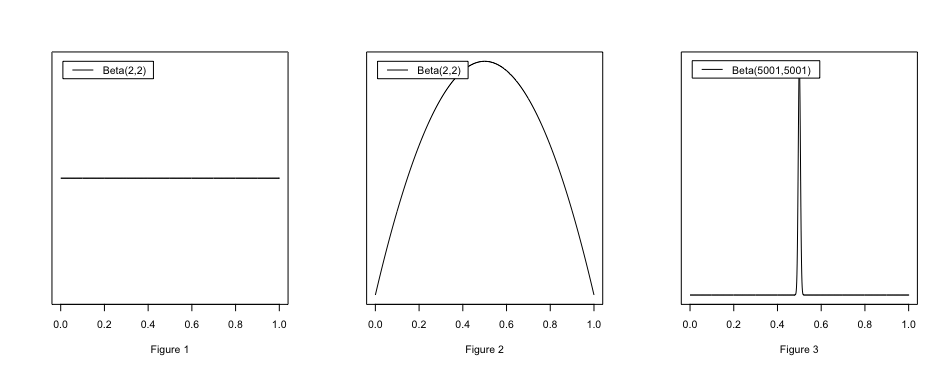
\includegraphics{beta.png}
\caption{Beta Distributions}
\end{figure}

Intuitively, we can think of the first distribution as representing your
state of belief about the probability of getting a head on the next
flip. This distribution is plotted in Figure 1: note that it is wholly
flat, capturing the sort of state of indifference that the Principle of
Indifference is supposed to capture: One finds no ground in thinking one
probability is more credible than another.

The second distribution can be seen as our state of belief after
witnessing 10 flips of the coin, and 5 turn up heads and 5 tails.
Naturally, the peak - the mode of the distribution - is at
\(\theta = 0.5\), which seems sensible, because it reflects the evidence
that exactly half of the samples are heads. But we can see that at this
stage we are quite uncertain about \(\theta\), evidenced by the width of
the distribution. While \(\theta = 0.5\) is the peak, there is a
substantial area covering \(\theta > 0.55\) and \(\theta < 0.45\).

The third distribution, modeling the state of belief after one million
trials with half of them being heads, is intended to be an approximation
of Popper's ideal evidence scenario. The peak is again at \(0.5\), but
this plot has a noticeably narrower spread: we are much more confident
in our assessment that the coin has an equal propensity to land on heads
as tails. Also notice that at this stage, any value of \(\theta\) other
than \(0.5\) are practically impossible after receiving the ideal
evidence.

To state these observations more precisely, we can calculate the exact
probability using the corresponding cumulative distributions. Since beta
distributions are continuous distributions, we can only deal with
intervals of values. Still, we can provide a reasonably close
approximations. For instance, conditional on the ideal evidence, we
would be absolutely sure that the probability is between 0.46 and 0.54,
and practically certain, with the probability of 0.95, that it is
between 0.49 and 0.51. The relevant probabilities are summarized in the
following table:

\begin{longtable}[]{@{}lrr@{}}
\toprule
Distribution & \(P(0.46<\theta<0.54)\) &
\(P(0.49<\theta<0.51)\)\tabularnewline
\midrule
\endhead
\(Beta(1,1)\) & \(0.08\) & \(0.02\)\tabularnewline
\(Beta(11,11)\) & \(0.29\) & \(0.07\)\tabularnewline
\(Beta(500001,500001)\) & \(1\) & \(1\)\tabularnewline
\bottomrule
\end{longtable}

Now, let \(E\) be the ideal evidence, \(X_1,…X_{1000000}\), where
\(\sum_{i=1}^{1000000}X_i = 500000\), and let \(\theta\) be the coin's
propensity to land on heads. We now see that the following inequality
holds, since the left-hand side is \(0.02\), and for the right it's
\(1\).

\[P(0.49<\theta<0.51) <  P(0.49<\theta<0.51|E)\]

To make things more official-sounding, perhaps we can describe this as
\emph{Higher Order Relevance(HOR)}. Recall Keynes's idea is that for
some evidence \(E\) and hypothesis \(H\)

\[\text{Evidence $E$ is relevant to $H$ if and only if }P(H) \neq P(H|E)\]

HOR takes this on step further and suggests that, in addition to \(H\)
and \(E\), consider specific values \(x\) and \(y\), where
\(0 \leq x \leq y \leq 1\)

\[\text{Evidence $E$ has a higher order relevance to $x\leq \theta \leq y)$ iff}\]
\[P(x\leq \theta \leq y) \neq P(x\leq \theta \leq y)|E)\]

Under this analysis, we can see that Popper's argument contains a
sleight of hand that shifts between two ways of thinking about N---the
next coin toss landing on heads---'s probability. The argument begins by
asking, rather innocuously, for your prior for \(N\), but the ideal
evidence \(I\) Popper immediately introduced is not for \(N\) but for
the hypothesis that \(\theta = 0.5\). Popper is reasonably explicit
about \emph{that}, but what he is not explicit about is \emph{this}: he
has convinced us that \(I\) is both evidentially ideal for and
conditionally relevant to \(\theta = 0.5\). That, however, is a
misdirection, because he immediately starts talking the conditional
probability on \(I\), \emph{not} of \(H_{0.5}\), but of \(N\).

While I think that HOR provides a sufficient response to Popper's
paradox, it is not quite the same as accounting for the phenomenon in
question. In fact, by focusing on overcoming the difficulty raised by
the paradox caused by an absurd amount of evidence, we might have
overlooked what is truly at stake: rarely, if ever, do we have ideal
evidence for any substantive hypothesis, so situations where we have an
overabundance of evidence is an incomplete benchmark for the adequacy of
the account. In fact, our analysis shows that when we have perfect
information, evidential weight essentially becomes a non-issue, because
it eliminates the uncertainty that calls for probabilistic reasoning to
begin with.

The important question, instead, is whether HOR can help with decision
making in situations where evidence is severely lacking. To this end, it
remains to be seen how higher order relevance can trickle down to first
order probability, on which decision making is based within the
classical Bayesian framework.

We need to, then, ask ourselves if HOR as a concept can make any
practical difference in decision making. It is in fact difficult to do
so within the basic framework of Bayesianism. To see this, imagine a
perverse game in which you will be shot to death if a coin flip lands on
head. Clearly, you don't want heads. You are given a choice between two
coins: the first coin \(P\) is similar to Popper's coin from the ideal
evidence scenario, except now the ideal evidence actually shows that
there is a slight bias in favor of heads, say the expected value is
0.51. The other coin \(U\) is one you have never seen before, so on an
ignorance prior your expected value \(E(\theta_U)\) is 0.5 . Now, which
would you choose? An argument can be made that you probably still want
the Popperian coin, because you know you are almost certainly getting
\(\theta_P = 0.51\). From the perspective of expected utility, however,
it is hard to rationalize such a decision, because the unknown coin
still has a lower expected value. That is,

\[\frac{510000}{1000000}> \frac{1}{2}\]

So it seems that we are back to where we started - the relevance
demonstrated on a higher order simply vanishes when we consider the
matter on the level of decision making, which is entirely based on a
precise point-estimate of the first order probability.

If the point estimate is to be blamed, the natural response is that we
do rely on an interval estimate instead. This solution is reminiscent of
the call to abolish the use of \(p\) values in Frequentist statistics,
and instead we should report the confidence interval of our findings.
The idea is that point estimates are inherently misleading, since they,
by design, summarize the data by discarding information such as higher
order relevance. This problem is somewhat analogous to the one we are
running into with respect to expected values. So one possible solution
is that we should only insist on making our decisions based on
\emph{credible intervals}, which is the Bayesian version of the
confidence interval. For instance, suppose
\(\theta_P \sim Beta(480000,520000)\) and \(\theta_U \sim Beta(1,1)\).
We can deduce that

\[P(0.479\leq \theta_P \leq 0.481) = 0.99\]
\[P(0.005\leq \theta_U \leq 0.995) = 0.99\]

\noindent In other words, we can say there is a 0.99 probability that
\(P\)'s propensity to land on heads is between 0.479 and 0.481
(practically 0.48) and for \(U\) it's between 0.005 and 0.995.

However, it seems to me that we are simply restating higher order
relevance in terms of credible intervals, without dealing with the crux
of the problem - unless we are rationally allowed to refuse to follow
the precise expected value, even if the weight of evidence is low, we
will always have to match it to our best point estimate, which is the
expected value. Of course, the point is not that HOR doesn't matter,
because intuitively it does. The point is rather that we need a richer
philosophical framework to rationalize this intuition.

\hypertarget{the-concept-of-resiliency}{%
\subsection{The Concept of Resiliency}\label{the-concept-of-resiliency}}

Skyrms credits Richard Jeffrey as the first who notices that Popper's
paradox brings light to the very idea of resiliency. Jeffrey points out
that once we stop fixating on the probability of \(N\), the next toss
coming up head, we can see that our state of belief prior receiving the
ideal evidence has a degree of malleability.\footnote{Richard Jeffrey,
  \emph{Logic of Decision} (McGraw-Hill, 1965), 184.} Consider, for
instance, instead of asking only for the probability of \(N\), we ask
the probability of the next 5 tosses coming up heads. Once we think
about how our belief responds to how these 5 tosses would act as
potential evidence, given our posterior state of belief, we have very
little choice but to believe that probability is \((0.5)^5\), but we
would be a lot less compelled to do so with the prior state of belief.

Skyrms has proposed the notion of \emph{resiliency} to capture Jeffrey's
observation in a generalized manner: even though evidential weight is
not reflected by the probability, it is captured by its stability. The
idea that there is a probabilistic representation for a stable state of
belief can be illustrated as follows: if I have in front of me an urn
\(U\), with an unknown proportion of black and white balls. If I
randomly draw 2 balls from it with replacement and find one ball for
each color, my intuitive estimate of the proportion of black balls would
sensibly be somewhere around 1/2. But my state of belief should be
relatively unstable: it would be irrational for me to fixate on this
estimate, especially new light of conflicting evidence. If I sample two
more balls from the urn and they are both black, it would make sense for
me to raise my estimate for the proportion of black balls to more than
1/2---perhaps to 3/4. But suppose I continue to sample from for 996 more
times. Out of the total 1000 draws, 500 are black. At this point a
sensible would be back to around 1/2, but unlike my state of belief
after only 2 samples, after 1000 samples my state of belief is
stabilized: suppose I sample again and I draw five black balls in a row.
Now, even though drawing 5 black balls in a row seems rather
extraordinary, against the body of my evidence it would not warrant me
to revise my belief in any significant measure.

The intuition here is that the increase in the amount of evidence,
expressed here in terms of the number of samples, corresponds to the
increase of stability of the estimate. Skyrms has introduced a notion
called the \emph{resiliency} to capture this intuition sense of
stability.

Conceptually, this is an attractive way to capture to notion of
evidential weight. Keynes' puzzlement about how relevance and weight
could come apart is addressed; When a belief \(B\) is resilient, the
conditional probability on some new evidence \(E\) should be
approximately the same, that is, \(P(B|E) \approx P(B)\), even if \(E\)
would be highly relevant were \(B\) not resilient. If, for instance, a
resilient belief is one where the weight of the evidence for it is high,
then it is a logical consequence that evidence could make a belief more
weighty without changing its degree, for the weight is in fact
stabilizing this particular value.

Nevertheless, how the resilience of a belief can make a practical
difference is yet to be explained. In fact, for the most part,
resiliency does not do much better than higher order relevance: within
the structure of expected utility calculus, a highly resilient belief
will still recommend the same action as a non-resilient belief with the
same expected value. Skyrms' original motivation for the concept,
however, provides an important clue: he intended the concept of
resiliency to explicate the concept of the laws of nature, so the idea
is that a probability statement \(A\) based on a law of nature is one
that remains resilient against various extreme scenarios. What this
means is that we are supposed to calculate likelihoods based on data
that \emph{might have happened}, and see whether \(A\) is resilient
against it.

\hypertarget{counterfactual-priors-and-hypothetical-data}{%
\subsection{Counterfactual Priors and Hypothetical
Data}\label{counterfactual-priors-and-hypothetical-data}}

The notion of resiliency opens the door to how counterfactual reasoning
can be relevant in Bayesian reasoning. The crucial point is that to see
how resilient a probability is, it is not something we can determine by
looking at data that we already have. We have examine what \emph{might
have happened}. So notwithstanding Lindley's rhetorical question:

\begin{quote}
Of what relevance are things that might have happened, but did
not?\footnote{Lindley and Phillips, ``Inference for a Bernoulli Process
  (a Bayesian View),'' 114.}
\end{quote}

Counterfactual considerations are relevant in deliberating on how a
chosen hypothesis \emph{would} respond in light of confounding
scenarios, so that we can decide if it is a worthy hypothesis and, if
chosen, how we ought to further probe it. More specifically, the weight
of evidence is puzzling, because it needs to be understood in the
context of abduction, since its goal is to give information about how we
ought to structure our inductive space.

Skyrms suggests that the resilience of a belief manifests itself as ``a
reluctance to change.''\footnote{Skyrms, ``Resiliency, Propensities, and
  Causal Necessity,'' 707.} He suggests that we can measure weight
directly in terms of the difference between prior and posterior
probabilities. Perhaps we can call this the measure of instability,
which signifies a lack of weight:

\[\text{Instability: }|P(X|E_j) - y|\]

Where \(j\) is in the set of \(n\) possible states of affairs,
\(E_1,..., E_n\). Skyrms' idea is that we should pick a \(j\) that
creates the biggest difference.

To see what this means, consider how resiliency can be demonstrated
using the beta distribution, though keep in mind that it is not meant to
be a generalizable result, since different distributions work
differently. In any case, recall that different sets of parameters can
produce the same expected value. For instance, consider \(Beta(1,1)\)
and \(Beta(5000,5000)\). Their expected values are, of course, the same,
since \(\frac{1}{2} = \frac{5000}{10000}\). But the second distribution
is way much resilient than the first. Suppose these are distribution
functions that represent the opinions of two different agents, but they
both receive the same piece of evidence \(Y\) from a Bernoulli process
such that \(Y=\sum_{i=1}^5 X_i=5\), that is, getting 5 heads in a row.
We do not have to do the calculation to see that they will respond to
the evidence pretty differently: the first agent will raise her
posterior expected value from \(1/2\) to \(6/7\). The difference is
\(.36\), which is a considerable increase.

The second agent's opinion, however, would barely be changed:

\[\frac{5005}{10005} - \frac{5000}{10000} = 0.00025\]

It is barely a rounding error. In fact, we can see that the second agent
would have to see 200 successes \emph{in a row} in order to raise the
credence by \(0.01\):

\[\frac{5000+200}{5000+5000+200} = 0.51\]

Notice that this analysis requires counterfactual thinking in two ways:
we have to consider what our priors \emph{would} be like in different
circumstances, and we have to consider its response to some hypothetical
data. This is why the weight of evidence is a dispositional commitment:
one is committed to respond to the the deliverance of experience in a
deliberate manner, as dictated by the model decided upon after
considering various counterfactual scenarios.

This way of understanding evidential weight provides an important
insight on the voluntaristic idea that degrees of belief ought to be
understood as taking up an epistemic commitment during the context of
abduction. To deliberate on the appropriate hypothesis to be accepted
provisionally, I have to know what \emph{practical difference} its
acceptance would make on my future conduct. To do so, I have to draw
deductive inferences based on various possible models that I could
possibly accept, based on various hypothetical scenarios that come up
during experiment.

To see what I mean, it might help to see the interaction between the
evidence and posterior probability directly---this is shown in the
figure. The x-axis represents the number of heads in a row, so the
higher x is, the more extreme the hypothetical evidence is. The y-axis
is the posterior probability after receiving the x heads out of x throws
as indicated by the x-axis.

\begin{figure}
\centering
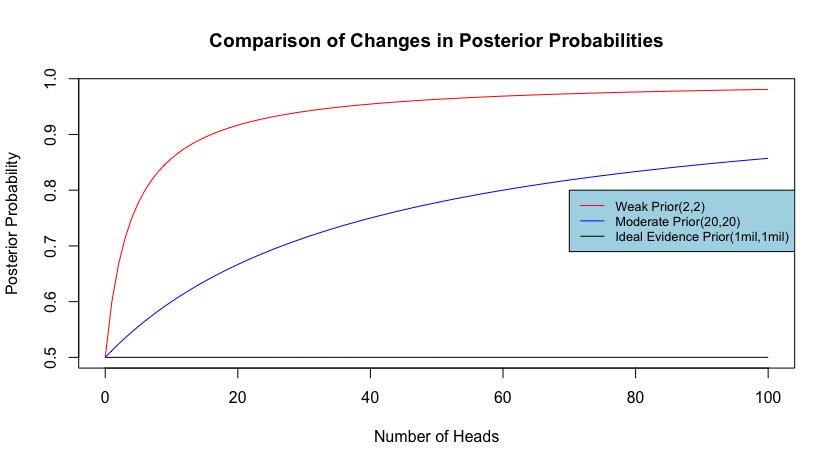
\includegraphics{rescompare.png}
\caption{Comparison of stabilities of different prior distributions:
values in parentheses are parameters for the beta distribution.}
\end{figure}

We see that these counterfactual priors behave quite differently in
slight of extreme evidence. Here, the weight of evidence clearly
corresponds to the sum of the parameters \(\alpha + \beta\), and the
higher it is, the less responsive it is to evidence. This is especially
clear when \(\alpha = \beta = 500\)---we see that with such as a weighty
prior distribution, it makes absolutely no difference how the extreme
the data is, until we get more than 60 heads in a row. Even if we tossed
100 out of 100, the expected value stays very close to \(0.5\). A ``flat
prior'', i.e., \(\alpha = \beta = 1\), is, as expected, not resilient
against almost any form of extreme evidence. The posterior is expected
to almost \(0.8\) after seeing 10 heads in a row, and rapidly approaches
unity.

From the deliberativist point of view, there is no \emph{a priori}
justification for one over another. There are circumstances in which the
extremely recalcitrant prior would be appropriate. Perhaps we can
consider the probability of a person's guilt based on the evidence. In
such a case, it would be rational to adopt a prior that is extremely
resilient, so that the posterior would be unresponsive unless the
evidence is beyond any reasonable doubt. Even in a less dramatic
situation such as testing the effectiveness of a drug, a resilient prior
could still be advisable when the result could mean have life-altering
consequences.

This also has an implication on the voluntarist interpretation of
degrees of belief. Recall that van Fraassen argues that assertions of
probability should not be a description of the agent's psychological
state. An argument for the voluntarist reading can be made in this
context. Suppose personally I think the coin is extremely likely to be
fair. It seems \emph{less} rational for me to adopt a prior to reflect
such a state, e.g., \(Beta(500,500)\); because, it would look as though
I am rigging the experiment in favor of \emph{my} hypothesis. The
rational thing, as a matter of fact, should be the opposite:
\emph{because} I am confident that my opinion is true, I am
intentionally adopting the opposite prior, with the assumption that the
data will overwhelm it. This is akin to a gambler with inside
information who is willing to make a bet with extremely unfavorable
odds. As the psychologist John Kruschke points out, it might be
advisable to choose a prior to satisfy a skeptic.\footnote{John K.
  Kruschke, ``Bayesian Estimation Supersedes the T Test,'' \emph{Journal
  of Experimental Psychology: General} 142, no. 2 (2013): 575.}

\hypertarget{introduction-1}{%
\section{Introduction}\label{introduction-1}}

\hypertarget{overview-1}{%
\subsection{Overview}\label{overview-1}}

In this dissertation, I defend the thesis that an epistemic judgment of
probability must be interpreted against the background of the
\emph{context of inquiry} in which it is made: in the abductive context,
judgments of probability are matters of \emph{decision}, made
strategically in service to the investigative goal of the inquirer; in
deduction, probabilities are \emph{derived} mathematically based on the
premises chosen in abduction, in order to explicate the implied
commitments the agent may incur from those decisions; during the
inductive stage, the inquirer is expected to conduct her empirical
investigation \emph{deliberately}, in accordance to the assertions and
decisions she made during abduction and induction, collectively referred
to as the \emph{deliberative context}.

In order to explore this particular notion of \emph{abduction} in the
context of formal epistemology, I will critically examine the
\emph{Reflection Principle}, proposed by Bas van Fraassen, as a guiding
principle of epistemic rationality. The principle, roughly, says that my
degrees of beliefs \emph{now} are rationally constrained by what I think
my future degrees of beliefs \emph{will be}. If you think tomorrow you
will judge that your degree of belief for rain is, say, \(0.5\), it
would irrational, the principle says, to assert that your \emph{current}
probability for the same event is anything other than \(0.5\).

To demystify Reflection and illuminate its connection to abduction, I
will devote chapter 2 for explaining van Fraassen's probabilist position
called \emph{voluntarism}. Basically, voluntarism rejects the Bayesian
idea that judgments of probability are \emph{descriptive} reports of the
agent psychological states. Instead, the voluntarist holds that to hold
a belief, partial or otherwise, is a matter of making a commitment to
stand by the belief in the future. It is, in a philosophically important
sense, analogous to making a \emph{promise}, which implies the
promiser's commitment to act in accordance to the content of the promise
in the future. Thus, judgments of probability, like making promises, are
what philosophers called \emph{speech acts}. To make the connection
between Reflection and abduction, I will provide a \emph{pragmatic}
interpretation of voluntarism. In particular, I appeal to Peirce's later
formulation of the Pragmatic Maxim that to accept a belief implies the
acceptance of the practical difference the relevant concepts'
contribution to the agent's \emph{deliberate conduct}.

In chapter 3, I will discuss this idea of deliberate conduct in the
context of philosophy of statistics. One of the many disagreements
between the Bayesians and frequentists is the relevant of the so-called
``stopping rules'', which designate when sampling will be stopped.
Traditionally, Bayesian statisticians argue that stopping rules are
problematic, because it takes into considerations of extra-statistical
facts---the agent's intention to stop. The traditional Bayesian line is
that Bayesian methods do not have to take into facts about the
experimenter's deliberations about how the experiment should run,
because Bayesian methods follow the so-called \emph{Likelihood
Principle}. I will argue that such an assumption is not correct: in
fact, like frequentists, Bayesians can also manipulate the statistical
result by changing their intentions to stop. I will propose that the
flight from intentions is not warranted; instead, we need a
philosophical account of how intentions are subjective to rational
evaluation in terms of epistemic commitments and obligations. I will
introduce the problem of stopping rule originates from the statistical
practice of Duke parapsychologists, and also consider a potential
objection to my argument based on a result regarding the value of
information proven by Frank Ramsey and I. J. Good.

One improvement of Reflection I will propose is that the commitment one
incurs from making an epistemic judgment ought to be understood not as
an unwavering perseverance in one's belief, but a disposition with
degrees of responsiveness to new experience. In other words, evidential
weight is a measure of one's \emph{dispositional commitment}: to put
oneself under the obligation to revise one's belief under different
evidential scenarios in a \emph{self-controlled} manner. Roughly, what I
mean is this: there are two senses in which my judgment that \$there is
a \(50/50\) chance that it will rain tomorrow have repercussion on . One
is to say I have the obligation to hold steadfastly on the belief, even
if I come to encounter evidence that suggests the contrary. On a rigid
understanding of the idea that accepting a belief is a commitment, this
might sound like the thing to do. The other, one that I think makes more
sense in the context of inquiry, is this: I incur a particular
\emph{vulnerability} to evidence. For instance, my commitment may be
such that though at this point my personal probability of rain is
\(0.5\), I am willing to revise my opinion based on a small amount of
evidence. This could be the commitment to have if I had no reason to
think one way or another, so that some evidence pointing to one way or
another is sufficient for me to be swayed. On the other hand, my
commitment in the probability of rain being \(0.5\) could be
\emph{weighty}: perhaps two meteorologists that I equally trust are each
giving completely conflicting forecast, such that I am in a state of
ambivalence that cannot be easily resolved, unless I find substantial
evidence to disqualify one of my sources as reliable. Reflection, for
the most part, does not address this. This will the be focus of chapter
4, in which I exploit the notion of the \emph{weight of evidence} in
explaining my proposal.

\hypertarget{motivation-1}{%
\subsection{Motivation}\label{motivation-1}}

Historically, empiricism is often associated with a flavor of
foundationalism that holds that empirical evidence must in some sense be
untainted - if experience is to serve as the objective foundation of
knowledge, it must be unsullied by our attitudes, beliefs, and values.
It is without a doubt motivated by a conception of rationality familiar
to philosophers, because of Descartes' method of doubt:

\begin{quote}
Reason now leads me to think that I should hold back my assent from
opinions which are not completely certain and indubitable just as
carefully as I do from those which are patently false.\footnote{Descartes,
  \emph{The Philosophical Writings of Descartes}, 1:17.}
\end{quote}

The idea is that it is irrational to hold unjustified opinions, and the
empiricist response is to find a way in which our knowledge can be
justified by some indubitable experience. Quine is arguably the last
great empiricist in this tradition, even though it is not immediately
obvious. In ``Epistemology Naturalized'', Quine describes what he takes
be `conceptual' and `doctrinal' cores of empiricist epistemology. The
conceptual core of empiricism, according to Quine, is concerned with the
explication of our concepts in terms of more ``basic'' concepts, which
refers directly to our sense experience, and the doctrinal side aims to
show that all of our justified beliefs can be inferentially traced to a
set of foundational and self-justified propositions.\footnote{Quine,
  ``Epistemology Naturalized,'' 70--78.} Even though Quine has claimed
to have jettisoned these traditional empiricist commitments, and
replaced them with a naturalized epistemology, he has not resolutely
renounced this empiricist project: his idea of epistemology naturalized
is simply to replace the old-fashioned notion ``experience'' with
physicalist equivalent that he deemed more scientifically respectable.
In his last major work, ``From Stimulus to Science'', he still pursues
the foundationalist project under the disguise of naturalism, by
suggesting ways in which the basis of science can be reduced to the
firing of neural receptors.\footnote{Quine, \emph{From Stimulus to
  Science}, 15--16.}

Such an attitude also permeates through the works of Carnap, another
great empiricist. \emph{The Logical Structure of the World}, also known
by its German title \emph{Aufbau}, is often considered by Quine as the
most thorough attempt to carry out the project of reductionism, as its
aim is ``a step-by-step derivation or 'construction' of all concepts
from certain fundamental concepts\ldots{}''\footnote{{\textbf{???}}}
Carnap the phenomenal reductionist is Quine's favorite philosophical
foil in virtually all of his work.

However, in the \emph{Aufbau} there is also an empiricist instinct that
is antithetical to foundationalism: one that emphasizes the role of
decision, intention, and volition in our practice of knowledge. Even
though Carnap spends the major of the \emph{Aufbau} to reduce all
concepts in a language of phenomenal experience, he explains that there
is nothing metaphysically necessary about this design decision---its
appropriateness depends ultimately on the decider's
``standpoint.''\footnote{{\textbf{???}}}

In \emph{The Logical Syntax of Language}, he codifies this normative
stance as \emph{the Principle of Tolerance}:

\begin{quote}
\emph{It is not our business to set up prohibitions, but to arrive at
conventions\ldots{} In logic, there are no morals.} Everyone is at
liberty to build up his own logic, i.e., his own form of language, as he
wishes. All that is required of him is that, if he wishes to discuss it,
he must state his methods clearly\ldots{}\footnote{Carnap, \emph{The
  Logical Syntax of Language}, 51--51.}
\end{quote}

This was evidently prompted by the disputes between logicians and
mathematicians regarding the ``correct'' language of logic. But the
standard of correctness does not exist until a language is chosen, so in
an important sense, trying to determine which language is better than
another is ultimately futile. However, once we adopt the Principle of
Tolerance, ``before us lies the boundless ocean of unlimited
possibilities.''\footnote{Carnap, xv, p.50.}

Carnap, I think, embodies two competing philosophical attitudes: one is
the desire for an algorithmic ideal of rationality, and the other is the
recognition that human rationality is full of gaps. The former point of
view demands the clarity of thought, so that each inferential step is
perfectly secure. The second stance, on the other hands, allows rational
leaps of faith take in the form of making conjectures beyond what is
necessarily implied by our evidence.

The goal of this dissertation can be summarized as a philosophical
exploration of the dynamics between these two styles of thinking within
the context of probabilistic reasoning. My main contention is that both
styles are thinking are needed to make sense of our rationality, and
their interaction must be understood in the respective role they play in
the different \emph{contexts} of inquiry.

The notion of inquiry is an explicit reference to the philosophy of C.
S. Peirce, whose view is an important basis of and inspiration to the
position I aim to defend and develop here. Peirce, as I understand him,
has a systematic understanding of the context-sensitivity of epistemic
judgments. That is, the evaluation of an assertion or a belief cannot be
detached from the context in which it occurs: an assertion of
probability has different normative implications in the context of
abduction, deduction, and induction. My main contention is that an
assertion has no normative force unless it is underwritten by an
epistemic practice that incentivizes the agent to stand by the
obligations imposed upon her.

\hypertarget{historical-context-1}{%
\subsection{Historical Context}\label{historical-context-1}}

How should probability constrain our beliefs? Can degrees of belief be
rational? There are question of a general epistemological interest.
However, within the rich history of probability, we find the major
figures also struggles with the two concepts of rationality described
above. In particular, we see that the dispute between J. M. Keynes and
F. P. Frank as one about whether we should understand the rationality of
degrees of belief as being prohibitive or permissive.

\hypertarget{rational-degrees-of-belief-1}{%
\subsubsection{Rational Degrees of
Belief}\label{rational-degrees-of-belief-1}}

Probability, in Keynes's view, is defined as a logical relation between
a premise and a conclusion. Probability relations are logical, because
this relation belongs to the same conceptual category as the entailment
relation between the premises and conclusion in a deductive argument.
Keynes says:

\begin{quote}
Inasmuch as it is always assumed that we can sometimes judge directly
that a conclusion follows from a premiss, it is no great extension of
this assumption to suppose that we can sometimes recognise that a
conclusion partially follows from, or stands in a relation of
probability to, a premiss.\footnote{Keynes, \emph{A Treatise on
  Probability}, 57.}
\end{quote}

Keynes' logical interpretation of probability has the advantage of
providing a direct explanation on why probability is \emph{normative}:
we \emph{should} reason in accordance to probability for the same reason
that we should respect a deductive rule like \emph{modus ponens}: the
degrees of a person's partial belief should correspond to the degree to
which the premises render the conclusion probable, whereas in a
deductive proof, one has to accept the conclusion as necessarily true,
were the premises true. Hence Keynes talks about probability not as
something we can attribute to a proposition, or one's attitude of it,
but a logical property of an argument.\footnote{There is a technical
  consequence for this. If probability is a relation, it follows that it
  never makes sense to talk about the probability of an event without in
  relation to any other proposition, so for Keynes all probabilities are
  conditional probabilities.}

As Frequentists often find little use for the idea of degrees of belief,
it is often seen as a notion exclusive to subjective theories of
probability; however Keynes' rational degrees of belief are supposed to
be objective relations independent of the human mind.

More important, in Keynes, we find the foundationalist attitude that he
inherited from the logical atomism of Russell. Keynes accepts Russell's
idea of knowledge by acquaintance: some propositions, such as ``I have a
sensation of yellow'', are justified by virtue of being perceptually
acquainted with it.\footnote{Keynes, 11--12.} Furthermore, acquaintance
yields not only knowledge of the senses, but also of logical relations:

\begin{quote}
When we know something by argument this must be through direct
acquaintance with some logical relation between the conclusion and the
premiss. In all knowledge, therefore, there is some direct element; and
logic can never be made purely mechanical. All it can do is so to
arrange the reasoning that the logical relations, which have to be
perceived directly, are made explicit and are of a simple
kind.\footnote{Keynes, 14.}
\end{quote}

This can be puzzling position, considering Keynes's goal is to develop a
formal system of probability, but If logical relations are not
analyzable in terms of empirical features, but an irreducible relation
knowable to us only by perception or intuition, then why would we need a
formal system? Keynes' answer is that everyone's intuitive faculty is
different, ``the perceptions of some relations of probability may be
outside the powers of some or all of us,'' so we need principles to make
these perception explicit and justified.\footnote{Keynes, 18.}

One important principle is the \emph{Principle of Indifference}. Laplace
is well-known for articulating a version of it:

\begin{quote}
When the probability of a simple event is unknown, one may suppose that
it is equally likely to take on any value from zero to one\ldots{} the
probability of each of these hypotheses, given the observed event, is a
fraction whose numerator is the probability of the event under this
hypothesis, and whose denominator is the sum of similar probabilities
under each of the hypotheses.\footnote{Laplace, \emph{Philosophical
  Essay on Probabilities}, 20.}
\end{quote}

In other words, when we are in complete ignorance regarding the outcome
of the event, the probability of each possible outcome is:

\[\frac{\text{1}}{\text{\# of total possible hypotheses}}\]

Many have criticized this principle. Peirce, for instance vehemently
rejects it, as he argues that in many cases, especially when the number
of possible outcomes is ambiguous, using the principle will lead to
contradictions. A simple example would be determining the probability of
an unknown object, for example, a marble, having a certain color, say,
red. Suppose I have no information about this marble, so I have no
reason to think the marble is red or not.\footnote{Assume that the cover
  of the book has only one color.} Following the principle, it would
seem that \(P(R) = P(\neg R) = 0.5\). However, we are led to
contradictions when we asks if the book is yellow, black, etc.; because,
using the same reasoning, we would say
\(P(Y) = P(\neg Y) = P(B) = P(\neg B) = 0.5\). The contradiction is that
these are mutually exclusive propositions, so axioms of probability say
that their sum cannot go beyond \(1\).

When Keynes wrote \emph{A Treatise on Probability}, he was keenly aware
of the sort of problematic consequences Peirce describes. However, he
thinks that the paradoxes only suggest that the principle is to be
restricted, not abandoned altogether. To begin, he notes that the
crucial terms used in the principle are not clearly defined:

\begin{quote}
The principle states that `there must be no known reason for preferring
one of a set of alternatives to any other.' What does this mean? What
are `reasons,' and how are we to know whether they do or do not justify
us in preferring one alternative to another? I do not know any
discussion of Probability in which this question has been so much as
asked.\footnote{Keynes, \emph{A Treatise on Probability}, 58.}
\end{quote}

Instead, he proposes that this clause ought to be explicated in terms of
conditional relevance. That is, to say that we have no reason to prefer
a proposition \(H\) over its alternatives is to say that there is no
evidence such that it is relevant to \(H\) but irrelevant to all the
alternatives. Roughly speaking, \(E\) is relevant to \(H\) on background
knowledge \(K\) if and only if: \[P(H|K) \neq P(H|K\wedge E)\]

According to Keynes, one necessary condition for a justified application
of Indifference is that for a set of \(n\) possible outcomes,
\(H_1,...H_n\), there is no evidential proposition \(E\) such that it is
conditionally relevant to some but not others.

The relevance criterion is necessary but not sufficient, because the
paradoxes need to be dealt with. He argues that the Principle of
Indifference should not be used when the alternatives under
consideration can be further analyzed, or, using his term,
``divisible''. Consider again the marble example. The paradox begins
with the assumption that red and not red are the two alternatives. While
it is true that these outcomes are exhaustive, ``not red'' should be
analyzed before we distribute the probabilities, since it also
encompasses the possibility that it is black, it is blue, etc. So
according to Keynes' conditions, judging \(P(R) = P(\neg R) = 0.5\) is
unjustified, since it is not a legal application of the Principle of
Indifference.

With Keynes' version of the principle, we have to know a great deal
about the setup of the sample space, before even entertaining the
possibility of indifference between alternatives. According to Keynes'
proposal, this means that most of our intuitive judgments of
indifference would be illicit. In fact, Keynes admits just as much: he
holds that in many if not most scenarios, the probability of a given
event cannot be given a precise value. For many propositions, it would
be impossible to say anything about their probability at all. Of course,
Keynes is not saying that it is psychologically impossible for us to
have degrees of belief for a proposition that fails to satisfy these
conditions, but he is saying that they would not be \emph{rational}
degrees of belief.

What I want to bring our attention is Keynes' epistemology behind his
theory of probability is fairly foundationalistic. That is, for Keynes
the Principle of Indifference is \emph{normative}. Keynes's view allows
the possibility that one could be mistaken in perceiving indifference,
and to accommodate that he has to rely on the Principle of Indifference
as a normative principle, which `endeavours to formulate a rule which
will justify judgments of \emph{indifference}.'\footnote{Keynes, 60.}
So, the principle serves as a standard of correctness by specifying the
conditions under which the uniform distribution of probability among
hypotheses is \emph{rational}, i.e., justified.

In his ``Truth and Probability'', Ramsey responds to Keynes's view by
rejecting the conception of degree of belief as perceptible logical
relations:

\begin{quote}
\ldots{}there really do not seem to be any such things as the
probability relations {[}Keynes{]} describes. He supposes that, at any
rate in certain cases, they can be perceived; but speaking for myself I
feel confident that this is not true. I do not perceive them, and if I
am to be persuaded that they exist it must be by argument; moreover I
shrewdly suspect that others do not perceive them either, because they
are able to come to so very little agreement as to which of them relates
any two given propositions.
\end{quote}

However, part of the appeal of Keynes' theory is that probability itself
is irreducibly normative, since they are objective and logical
relations. It would seem that denying the existence of these logical
relations also robs probability its normative force. Ramsey recognizes
this, and explicitly rejects both the Principle of Indifference and
Keynes' strongly normative conception of rational degrees of belief.

To begin, Ramsey points out that the reason Keynes's position
\emph{requires} principles such as Indifference is that he holds that
degrees of belief must be \emph{justified} before it can be admitted in
the calculus of probability; however, Ramsey thinks that such a demand
cannot be satisfied:

\begin{quote}
\ldots{}to ask what initial degrees of belief are justified\ldots{}
seems to me a meaningless question; and even if it had a meaning I do
not see how it could be answered.\footnote{Ramsey, \emph{Philosophical
  Papers}, 88.}
\end{quote}

Once this requirement of rationality is jettisoned,

\begin{quote}
the Principle of Indifference can now be altogether dispensed with; we
do not regard it as belonging to formal logic to say what should be a
man's expectation of drawing a white or a black ball from an urn; his
original expectations may within the limits of consistency be any he
likes; all we have to point out is that if he has certain expectations
he is bound in consistency to have certain others. This is simply
bringing probability into line with ordinary formal logic, which does
not criticize premisses but merely declares that certain conclusions are
the only ones consistent with them.
\end{quote}

Thus Ramsey recognizes the normative nature of Keynes' use of the
principle: it constrains our beliefs such that when the conditions for
Indifference are met, you \emph{should} assign equal probabilities to
the outcomes, otherwise you are \emph{irrational}. As the quote above
makes clear, Ramsey's view makes no such demand. As far as he is
concerned, it is not probability's business to tell people what degrees
of belief they \emph{should} have. Instead, the normative force of
probability is the same as that of deductive logic: it serves as a tool
of checking consistency of a set of beliefs, and no more.

Ramsey, then, is advocating what came to be the standard notion of
Bayesian rationality: coherence. The question has shifted from ``what
are rational degrees of belief?'' to ``is this set of partial beliefs
consistent?'' Ramsey's analogy to deductive logic is helpful. Consider
this argument:

\begin{enumerate}
\def\labelenumi{\arabic{enumi}.}
\tightlist
\item
  All Chinese are Martians.
\item
  Socrates is Chinese.
\item
  \(\therefore\) Socrates is a Martian.
\end{enumerate}

Even though the argument contains all false claims, from a deductive
perspective, it is a perfectly valid argument. In the same way, if we
have a definitely fair coin but an agent decides that
\(P(Heads)=0.999\), she is still rational as long as she also believes
\(P(Tails) = 0.001\). This normative point is perhaps the most
influential among the ideas from ``Truth and Probability,'' as Ramsey
gestures toward the use of Dutch book arguments in support of coherence
as a requirement of rationality: anyone who violates the axioms of
probability ``could have a book made against him by a cunning better and
would then stand to lose in any event.''\footnote{Ramsey.} The argument
is based on the assumption that the agent's willingness to bet is based
her degrees of belief and utility function, so an inconsistent set of
partial beliefs would imply contradictory betting behavior that could be
exploited.

For instance, if the agent believe than \(P(Heads) = 0.999\) yet also
simultaneously holding that \(P(Tails) = 0.5\) This means, based on the
assumptions required by Dutch book arguments, you would be willing to
pay respectively \$0.999 and \$0.5 for a bet that pays \$1. So, if a
bookie offers the agent both bets at those prices, which comes to the
total of \$1.499, these bets should appear to be fair, based on her
degrees of belief. But she is guaranteed to lose money from this deal,
since landing on heads and on tails are mutually exclusive, she will win
at most \$1, so she lose \(1.499 - 1 = 0.499\) for sure. This is due to
the fact that she violates the axiom of probability that says that the
sum of the probability of each possible outcome has to be
\(1\).\footnote{Hajek, ``Dutch Book Arguments,'' 176.}

I do not wish to dispute the effectiveness of Dutch book arguments here.
Let us for the sake of argument assume that probabilistic coherence is a
basic requirement of rationality, because the problem I would like to
address is aspects of rationality unaccounted for in Ramsey's view, even
if we grant the use of Dutch book arguments, that is, is coherence a
sufficient substitute for a normative conception of degrees of belief?
L. J. Savage, a strong advocate of Bayesianism and subjective
probability, expresses his doubts about whether consistency is enough:

\begin{quote}
According to the personalistic view, the role of the mathematical theory
of probability is to enable the person using it to detect
inconsistencies in his own real or envisaged behavior. It is also
understood that, having detected an inconsistency, he will remove it. An
inconsistency is typically removable in many different ways, among which
the theory gives no guidance for choosing.\footnote{Savage, \emph{The
  Foundations of Statistics}, 57.}
\end{quote}

Savage's point can be illustrated by considering the Dutch book case
above: suppose the subject is convinced that her degrees of belief,
\(P(Heads) = 0.999\) and \(P(Tails) = 0.5\) are incoherent: what
normative conclusion should she draw from this? The only advice Ramsey
could give her is that they should add up to 1, but should she lower
\(P(Heads)\) to \(0.5\) or lower \(P(Tails)\) to \(0.001\)? In fact,
there are, quite literally, infinite ways to for her to resolve the
inconsistency. This illuminates the lacuna left open by a descriptive
understanding of degrees of belief, motivated by both an operationalist
understanding of pragmatism and a rejection of Keynes' rational degrees
of belief. In Keynes' framework, assuming that the conditions for the
Principle of Indifference are satisfied, the \emph{only} rational way to
evaluate these probabilities is \(P(Heads) = P(Tails) = 0.5\).

In the paper, Ramsey struggles with this issue: at the end he arrives at
a somewhat vulgar pragmatism that says that an opinion is reasonable
insofar as it works more often than not.\footnote{Ramsey,
  \emph{Philosophical Papers}, 93.} Keynes' assessment of his debate
with Ramsey is telling:

\begin{quote}
{[}According to Ramsey,{]} the basis of our degrees of belief\ldots{} is
part of our human outfit, perhaps given us merely by natural selection,
analogous to our perception and our memories rather than to formal
logic. So far I yield to Ramsey---I think he is right. But in attempting
to distinguish ``rational'' degrees of belief from belief in general he
was not yet, I think, quite successful. It is not getting to the bottom
of the principle of induction merely to say that it is a useful mental
habit\footnote{Keynes, \emph{Essays in Biography}, 300--301.}
\end{quote}

The lesson I want to draw from the dispute between Keynes and Ramsey is
this: one of crucial questions regarding the rationality of partial
belief is the rational status of our prior opinions. Keynes, at least in
regard to probabilistic judgments, holds that degrees of belief can be
rational only if they are ultimately justified by some logically
determined and objective priors. The result is a highly skeptical
attitude toward the feasibility of having precise degrees of belief for
most cases. Ramsey's plea for merely reasonable degrees of belief could
be see as the rejection of such a requirement, but, as Keynes points,
this proposal is inadequate unless we can find alternative ways to
articulate the criteria of rationality for degrees of belief. Orthodox
Bayesianism and Voluntarism, the two competing views central to the
discussion in chapter 2, can be seen as two ways in which this need can
be addressed.

\hypertarget{bayesianism-and-voluntarism-1}{%
\subsubsection{Bayesianism and
Voluntarism}\label{bayesianism-and-voluntarism-1}}

In \emph{The Will to Believe}, van Fraassen tries to offer a version of
probabilism that is distinct from Bayesianism. In the context of formal
epistemology, \emph{probabilism} can be characterized as the following
two theses:

\begin{enumerate}
\def\labelenumi{\arabic{enumi}.}
\tightlist
\item
  The strength of a belief can be measured numerically as \emph{degrees
  of belief}.
\item
  The rationality of degrees of belief is governed by the axioms of
  probability.
\end{enumerate}

Even though `probabilism' is often used as a synonymy for `Bayesianism',
van Fraassen makes a subtle distinction between the two:

\begin{quote}
So: I am a probabilist, though not a Bayesian. Like the Bayesian I hold
that rational persons with the same evidence can still disagree in their
opinion generally; but I do not accept the Bayesian recipes for opinion
change as rationally compelling. I do accept the Bayesian extension of
the canons of logic to all forms of opinion and opinion
change.\footnote{Fraassen, \emph{Laws and Symmetry}, 1989, 175.}
\end{quote}

Evidently, he is taking ``probabilism'' to be a broader term than
``Bayesianism''. In particular, Bayesianism addresses the following
issues on top of probabilism:

\begin{enumerate}
\def\labelenumi{\arabic{enumi}.}
\tightlist
\item
  The rationality of our \emph{existing} opinions and,
\item
  The rational procedure to \emph{revise} these opinions.
\end{enumerate}

What van Fraassen calls \emph{Orthodox} Bayesianism satisfies the second
by holding that the only justifiable way to revise one's opinion is
through Bayes' theorem.\footnote{To be more precise, we should also
  distinguish \emph{epistemic} Bayesians and \emph{statistical}
  Bayesians. In this paper, I follow van Fraassen in using the term
  `Orthodox Bayesian' to describe an epistemological position that holds
  a strict view on belief revision just described. A Bayesian
  \emph{statistician} might think that belief do come in degrees and
  that Bayesian statistics is the best framework for drawing statistical
  inferences, but she might not think that all beliefs can be
  meaningfully given a Bayesian analysis.} This is often codified as the
so-called rule of

\begin{quote}
\emph{Conditionalization}: one is rationally compelled to update one's
prior degree of belief for \(H\) in light of the acquisition of relevant
evidence \(E\) via the application of Bayes' theorem, which determines
the posterior opinion degree of belief \(P(H|E)\).\footnote{Fraassen Bas
  C., ``Belief and the Problem of Ulysses and the Sirens,'' 17.}
\end{quote}

Conditionalization, of course, does not say anything about the rational
status of existing opinions, i.e., priors. Orthodox Bayesians, in this
regard, are subjective Bayesians: priors do not have to be justified.
From the epistemological perspective, this is a move against skepticism,
for it rejects the assumption that knowledge and rationality presupposes
the ability to justify all of my existing opinions. In other words,
Orthodox Bayesians side with Ramsey in rejecting that degrees of belief
must be justified to be rational.

Using Peirce's terminology, which van Fraassen adopts,
conditionalization is an \emph{explicative} procedure, which does not go
beyond what's implied by facts and logic, as opposed to be being
\emph{ampliative}, which extrapolates beyond them.\footnote{Peirce,
  ``The Probability of Induction.'' 297} We already saw the same idea
from Ramsey, who sees the normative role of probability as the logic of
consistency between partial beliefs. Orthodox Bayesianism, however,
further legislates the rational revision of belief by imposing
conditionalization, which fills the normative gap pointed out by Savage
and Ramsey. So, instead of Ramsey's ``useful mental habits'', Orthodox
Bayesians regard the ideal Bayesian agent, who revises her belief by
following conditionalization, as the standard of rationality. As van
Fraassen engagingly puts it, this purely explicative conception of
belief revision allows the Orthodox Bayesian ``to live a happy and
useful life by conscientiously updating the opinions gained at his
mother's knees, in response to his own experience.''\footnote{Fraassen,
  \emph{Laws and Symmetry}, 1989, 178.} This is assuming that
conditionalization will allow a set of initially diverse priors to
eventually converge into the same posterior.

Van Fraassen, however, rejects the idea that the ideal Bayesian agent is
the \emph{only} model of rationality. In particular, he insists that
rationality cannot be wholly reduced to following an explicative rule.
The result is an expanded notion of rationality. This alternative
conception of rationality maintains that:

\begin{quote}
what is rational to believe includes anything that one is not rationally
compelled to disbelieve. And similarly for ways of change: the rational
ways to change your opinions include any that remain within the bounds
of rationality---which may be very wide. \emph{Rationality is only
bridled irrationality.}\footnote{Fraassen, 171--172.}
\end{quote}

Van Fraassen calls his position \emph{voluntarism}, so let us call the
voluntaristic conception of rationality. It is voluntaristic in the
sense that an agent is free to adopt any opinion that is ``within the
bounds of rationality''.

At a glance, van Fraassen does not seem to be offering anything
different than Ramsey's coherentism. It sounds as though we are simply
returning the subjectivist idea that priors do not have to be justified.
But van Fraassen's view is actually subtler than that, and to see this
we must understand the pragmatist root voluntarism has.

Van Fraassen does not claim to be a pragmatist, but he credits James as
the originator of his voluntarism, which, in its most naive formulation,
says that the acceptance of belief is a matter of the will, that is, to
believe a proposition is to make a \emph{decision} to believe the
proposition. Unsurprisingly, this is traditionally a theological
position, which is the context of \emph{the Will to Believe}. Pascal's
Wager is the \emph{locus classicus} of voluntarism: the belief in God,
Pascal tells us, cannot be resolved by the appeal to evidence or reason;
instead, it is more akin to making a decision based on expected utility.
Because we gain infinite utility from believing in God correctly and
losing very little otherwise, the argument goes, the rational thing is
to decide that God exists.\footnote{``Pascal's Pensées,'' sec. 233.}

To be clear, my intention is not to deal with the theological issues
here, but the difficult task at hand that is to explain how van Fraassen
puts forth voluntarism as a general epistemological position about
degrees of belief. To go from Pascal to van Fraassen, we must understand
how James develops his voluntarism in response to Clifford.

Clifford, at least as characterized by James, is arguing for a standard
of rationality on which the acceptance of a proposition without
sufficient evidence is irrational, \emph{even if the proposition were
true}. Clifford is clear that this epistemic duty is categorical: ``It
is wrong always, everywhere, and for every one, to believe anything upon
insufficient evidence.''\footnote{James, \emph{The Will to Believe and
  Human Immortality}, 8.} To van Fraassen, this is paradigmatic example
of a compulsory conception of rationality.\footnote{Fraassen, \emph{Laws
  and Symmetry}, 1989, 171.} According to this picture of rationality,
what is rational to believe for a person is restricted to those for she
has justification, which could be in the form of evidence or logical
necessity. This, without a doubt, is motivated by same intuition about
rationality that motivated the traditional empiricists.

James argues against Clifford's view by introducing epistemic values
into the discussion: James suggests that we are pulled in two directions
in the formation of our opinions:

\begin{quote}
There are two ways of looking at our duty in the matter of
opinion\ldots{} \emph{We must know the truth; and we must avoid
error},--- these are our first and great commandments as would-be
knowers; but they are not two ways of stating an identical commandment,
they are two separable laws.\footnote{James, \emph{The Will to Believe
  and Human Immortality}, 17.}
\end{quote}

Why are they separate? Consider two types of epistemic agents: a greedy
truth-seeker and a unmovable skeptic. The former is driven by nothing
but the hunger for information, while the latter would rather accepts
nothing that is short of being absolutely certain. To satisfy their
respective values, their epistemic policies would be quite different:
the truth-seeker should maximize her true beliefs by believing in
everything, including contradictions and other falsehood. A skeptic can
avoid all errors by refusing to believe in anything. So, not only are
the desire for truth and the aversion to errors two separate epistemic
values, they lead to epistemic policies that are diametrically opposed
to each other.

These extreme epistemic policies seem absurd to us, because, we regard
both the attainment of truth and the avoidance of error as being
valuable. Satisfying one, however, often undermines another, due to our
limited resources: if we had infinite cognitive power, memory, and time,
we could perhaps learn in a way that guarantees the accuracy of our
information. But this is not what our epistemic life is like: we lack
the resource to fully fulfill these competing concerns: reaching for the
truth often means opening oneself to the risk of error, and to be
cautious against believing falsehood often lowers one's chance of the
truth. As a result, we are forced to find a measure of balance.

From an argumentative point of view, the purpose of James' introduction
of epistemic values is to frame Clifford's position in a new light. That
is, Clifford's call to suspend one's judgment is motivated by the
\emph{decision} to take priority in the avoidance of error over the the
desire for truth.

\begin{quote}
"he who says `Better go without belief forever than believe a lie!'
merely shows his own preponderant private horror of becoming a dupe. He
may be critical of many of his desires and fears, but this fear he
slavishly obeys\footnote{James, 18.}
\end{quote}

To agree with Clifford, then, one must decide that the price of the
security of skepticism is missing out on a chance in receiving the
truth---this is especially prominent in Clifford's insistence that it is
better to suspend judgment to accidentally come into the possession of a
true belief. But in some context, this seems hardly the rational course
of action:

\begin{quote}
It is like a general informing his soldiers that it is better to keep
out of battle forever than to risk a single wound.\footnote{James, 19.}
\end{quote}

What James is arguing, then, that Clifford's position presupposes that
the avoiding the risk of error is \emph{always} more important than
knowing the truth. James seems to be suggesting that, in theological and
moral matters, this cannot be the right, since these questions always
have a high degree of \emph{urgency}, and his contention is that in such
a situation, one has the right to accept these beliefs, as long as they
are committed to make the practical difference implied by the acceptance
of these beliefs.

It is clear that van Fraassen aims to create a contrast between James
and Clifford in service of his alternative to Orthodox Bayesianism. In
James' view, we find an argument for a more permissive notion of
rationality that makes room for leaps of faith that are not possible
under the algorithmic view of rationality depicted in Orthodox
Bayesianism. Of course, this is not quite sufficient, van Fraassen must
explain how rationality can be maintained when ampliative extrapolations
are allowed. This is the crucial topic for the next chapter, to which we
shall now turn.

\hypertarget{reflection-principle-and-the-pragmatic-maxim-1}{%
\section{Reflection Principle and the Pragmatic
Maxim}\label{reflection-principle-and-the-pragmatic-maxim-1}}

Should my current opinions be constrained by what I expect myself to
belief in the future? This is the concern addressed by the principle of
Reflection, which answers affirmatively:

\begin{quote}
\emph{General Reflection Principle.} My current opinion about event
\(E\) must lie in the range spanned by the possible opinions I may come
to have about \(E\) at later time \(t\), as far as my opinion is
concerned.\footnote{Fraassen Bas C., ``Belief and the Problem of Ulysses
  and the Sirens,'' 16.}
\end{quote}

In the context of probabilistic judgment, Reflection implies that your
current credence, i.e., subjective probability, for the proposition
\(K\) now at \(t1\) must be one of the values you consider as possible
in the future at \(t2\). Van Frassen formulates this general version of
the principle in order to accommodate imprecise probabilities and vague
opinions. I put leave issues regarding imprecise probabilities aside:
when talking about probability, in our context it is sufficient to a
version of Reflection that presupposes precise probability:

\begin{quote}
\emph{Special Reflection Principle.} \(P_t(E|p_{t+x} (E) = r)=r\)
\end{quote}

In words, this formulation says: your subject probability for \(E\)
currently at \(t\), given in the future at time \(t+x\) it will be
\(r\), should also be \(r\). For example, if tomorrow you will come to
believe that the probability of rain is \(0.5\), then your current
probability of rain should also be \(0.5\).

Why should what I think I will believe in the future constrain my
current opinion? The main purpose of this chapter is to demystify
Reflection. In particular, I shall argue for the novel view that
Reflection is a principle of \emph{abductive} reasoning: it regulates
the rationality of the epistemic judgments made in the context of
abduction. My contention is that Reflection is a guiding principle of
what Peirce calls the rationality of deliberate conduct. One criticism
of voluntarism I will focus on is that it does not recognize the
importance of the context sensitivity of epistemic judgment.

\hypertarget{moores-paradox-and-self-sabotaging-1}{%
\subsection{Moore's Paradox and
Self-Sabotaging}\label{moores-paradox-and-self-sabotaging-1}}

I have presented a contrast between Orthodox Bayesianism and van
Fraassen's voluntarism, by suggesting that conditionalization provides a
rational constraint that is explicative in nature, while voluntarism
allows ampliative extrapolation beyond the implication of the evidence.
Still, even if voluntarism presupposes a more liberal conception of
rationality, it must impose least \emph{some} constraints on our
beliefs. This is what the Reflection Principle is supposed to do; it
aims to replace conditionalization as the overarching principle of
rationality; however, what how we conceive our future selves has to do
with rationality is still rather mysterious. To understand this, we have
to consider the implication of violating Reflection. The possibility of
being Dutch-booked is part of it, but not the full story. The crucial
idea is how the violation of Reflection can lead to the so-called
``Moore's Paradox.''

To begin, we have to distinguish a Moorean \emph{absurdity} and Moore's
\emph{paradox}. A Moorean absurdity arises when a person utters or
thinks that `\(P\) and I don't believe that \(P\)'. For example,

\begin{quote}
\begin{itemize}
\tightlist
\item
  It's raining but I don't believe that it is.
\end{itemize}
\end{quote}

Logically speaking, such an utterance or thought is not contradictory.
There is no logical connection between my belief in the rain and whether
it is actually raining. This can be demonstrated easily by rephrasing
the same proposition from a third person point of view:

\begin{quote}
\begin{itemize}
\tightlist
\item
  It's raining but Lok doesn't believe that is.
\end{itemize}
\end{quote}

Unlike the former, this could easily be a statement about an error on my
part. Moore's \emph{paradox} is the thought that, even though logic
tells us that such a proposition is perfectly consistent, it seems
absurd for anyone to \emph{assert} such the first-person-perspective
version of the proposition.\footnote{S. and N., \emph{Moore's Paradox},
  190.} The source of absurdity is from the conjunction of someone
asserting that it is raining, and the disavowal of the belief in what
she just asserts. Another way to phrase the paradox without appealing to
assertion is to say that a Moorean absurdity is a proposition that is
logically consistent but not believable. That is, I cannot, without
succumbing to absurdity, attribute to myself the belief that it's P and
I don't believe that P.

What does the possibility of Moorean absurdity suggest? According to one
analysis of the notion of absurdity, it is the result of a violation of
established norms. That is, there are implicit standard that govern the
norms between asserting \(P\) and believing \(P\), such that one is
expected to believe what she asserts. Of course, this is not to say that
people do not make deceptive assertion. In such a case the norms are
being exploited for various reasons, but in those cases the speakers do
not announce their intention to deceive. The absurdity comes from the
fact that the norms are being explicitly broken.

One explanation for Moore's paradox is that it signifies a violation of
the underlying norms for a \emph{speech act}. The idea is that many of
our linguistic practices carry non-linguistic effects beyond the content
of what's being said. Consider a classic example of a speech act: making
a promise. Speech acts theorists argue that there is a normative link
between uttering ``I promise that \(p\)'' and the intention to bring
about \(p\) in the future. A promise could be deemed infelicitous, when
a speaker fail to fulfill the normative conditions necessary for the act
of promising to be successful. Consider J. L. Austin's example: ``I
promise to do \(X\) but I do not intend to do it\footnote{Austin,
  \emph{How to Do Things with Words}, 54.} Like''\(P\), but I do not
believe \(P\)", this proposition appear absurd, because they violate the
implicit norm that when one makes a promise, she is expected to have the
sincere intention to fulfill the said promise.

More important, the expression of the intention implies that the
promisor is willingly placing oneself under an obligation to the
promisee.\footnote{Searle, \emph{Speech Acts}, 60.} So to make the
promise, while simultaneously expressing the lack of intention to carry
it out is an absurd act of \emph{self-sabotaging}. In the last section,
we saw that the voluntaristic conception of rationality holds that any
belief that is with the ``bounds of reason'' is rational. Van Fraassen
does not clearly define what those bounds are, but he does spell out
some specific conditions. One is that self-sabotaging is always
irrational, which depends on a distinction between \emph{ex post} and
\emph{ex ante} notions of rational evaluation:

\begin{quote}
Any act of decision can be evaluated in two ways. if we evaluate it
beforehand, we ask how \emph{reasonable} it is, and, afterward, we ask
to what extent it was \emph{vindicated}\ldots{} Therefore a minimal
criterion of reasonableness is that \emph{you should not sabotage your
possibilities of vindication beforehand}\footnote{Fraassen, \emph{Laws
  and Symmetry}, 1989, 157.}
\end{quote}

For instance, a promise could be unreasonable if the action required to
fulfill the promise is impossible, since this means the promiser will
never be vindicated. On the other hand, people do make insincere
promises, and sometimes that would be the rational thing to do: I could
be vindicated in making a insincere promise, If it turned out that doing
saved my life; however, my promise would be absurd, if I were to make an
insincere promise \emph{and} announce my insincerity.

Van Fraassen's contention is that a probabilistic judgment, for example:

\begin{quote}
\begin{itemize}
\tightlist
\item
  It seems more likely to me---supposing that it stays this cold---that
  it will snow than that it will rain.
\end{itemize}
\end{quote}

is more like the speech act of making a promise than a statement of
fact.\footnote{Fraassen, ``Belief and the Will,'' 1984, 252--255.} To
begin, we can consider what it would mean for a probabilistic judgment
to be a statement of fact. Ramsey's operationalist definition, as
discussed in the last chapter, seems to fit the bill: an
autobiographical report of one's degrees of belief, elicited through a
combination of neutral propositions and utility evaluation, is a causal
effect of the reporter's disposition to act, so a probabilistic judgment
is interpreted as a description of the agent's psychological state, much
like reports of an object's responses to being scratched by different
substances are descriptions of the object's hardness.

In contrast, consider a passage, which van Fraassen cites approvingly,
from Bruno De Finetti, another progenitor of modern Bayesianism:

\begin{quote}
Any assertion concerning probabilities of events is merely expressing of
somebody's opinion and not itself an event. There is no meaning,
therefore, in asking whether such an assertion is true or false or less
probable.
\end{quote}

\begin{quote}
The situation is different, of course, if we are concerned not with the
assertion itself but with whether ``somebody holds or expresses such an
opinion or acts according to it''; for this is a real event or
proposition.\footnote{Finetti, \emph{Probability, Induction, and
  Statistics}, 189.}
\end{quote}

De Finetti's distinction can be phrased within the framework of speech
acts theory: it is a statement of fact that Lok Chan made a promise to
do \(X\) today at 5PM. It would be true if I did make such a promise,
but it makes no sense to ask if the promise itself is true. I can make a
successful promise by clearly expressing my intention to fulfill my
obligation. De Finetti appears to be saying something quite similar: an
assertion is an \emph{expression} of opinion that itself cannot be true
or false.

In agreement with De Finetti, Van Fraassen argues that making a
probabilistic judgment is more like making a promise and reporting an
autobiographic report about one's psychological state. To make this
argument, van Fraassen tries to demonstrate that this statement

\begin{quote}
\begin{itemize}
\tightlist
\item
  my current degree of belief for \(A\) is \(x\), but I expect it to be
  a different value \(y\) in the future.
\end{itemize}
\end{quote}

to be an instance of a Moorean absurdity. More specifically, anyone who
asserts the above is said to be \emph{self-sabotaging}. It is evidently
much less clear that the violation of Reflection is an absurdity,
compared to making a promise while announcing the lack of intention to
keep it. To begin, perhaps we can first consider the violation in case
of full belief. Suppose I am invited to the flat earth society meeting
tomorrow that features an extreme persuasive speaker for the flat earth
theory. Knowing that I am always easily swayed by impressive rhetoric, I
assert that

\begin{quote}
\begin{itemize}
\tightlist
\item
  The earth is spherical but I expect to believe in a flat earth
  tomorrow.
\end{itemize}
\end{quote}

Am I sabotaging myself? The point is that if I am willing to assert
fully that the earth is spherical now, I should be able to stand by my
assertion in the future. If I know I will have some perfectly good
reasons to change my mind about it, then I really should not make that
assertion, since I know I will not be able to uphold it. Analogously, if
I make a promise today, it is implied that I will keep the promise
tomorrow, and a promise shouldn't keep considered as successful if I
know perfectly well that I cannot keep my it.

Furthermore, if I am committed in holding my belief in a spherical
earth, then I should simply avoid going to the meeting due to my
irrational weakness to rhetorics, in which case I do not expect to
believe in flat earth tomorrow. Analogously, if I made a promise to
someone that I shall never drink alcohol again, I am sabotaging myself
by intentionally putting myself in a situation that will cause my
promise to be broken.

The idea, then, is that making an assertion puts the agent under an
obligation to defend and rationally cultivate the proposition being
asserted. This makes enough sense for full belief, but there is a gap in
carrying this analysis over to degrees of belief. He clearly wants to
extend this reasoning to degrees of belief, so there must be a practical
difference between asserting my degree of belief for \(P\) to be 0.3 and
0.7.

Van Fraassen uses betting behavior and Dutch book arguments to fill this
gap.\footnote{Fraassen, ``Belief and the Will,'' 1984, 244.} The idea is
that asserting a judgment of probability requires me, quite literally,
to put money where my mouth is, and the money involved should be
directly proportional to my degrees of belief. This means that
Reflection implies that what I think my willingness will be in the
future should be my willingness to bet now. Van Fraassen shows that
violating in Reflection will lead to the susceptibility to a so-called
Dutch book, which is a set of bets that will lead to a guaranteed loss
for anyone who accepts it. A Dutch book \emph{argument} is aimed to
demonstrate that the vulnerability to Dutch books a sign of incoherence
and, therefore, irrationality. A Dutch book argument can be made in
support of Reflection by showing that by violating this principle, one
is opening oneself to being ``Dutchbooked''.

More specifically, the argument for Reflection requires a
\emph{Diachronic} Dutch book, which involves a Dutch book
\emph{strategy} to offer the agent bets that would be fair to the agent
at the time, but the acceptance of them will ultimately lead to a loss
to the agent. The trick is to ask the agent to bet on her opinion about
what her future opinion about \(E\) will be, in addition to offering
bets on her opinion about \(E\) itself. If the agent gives an answer
that violates Reflection, then the bookie will be able to make a Dutch
book against her, by offering bets that are fair to her according to her
credences at the time. This is supposed to show that violating
Reflection is an act of self-sabotage. The Dutch book argument will be
elaborated with technical details in the next subsection. It can be
skipped without loss of continuity.

\hypertarget{dutchbook-argument-for-reflection-1}{%
\subsection{Dutchbook Argument for
Reflection}\label{dutchbook-argument-for-reflection-1}}

A Dutch book involves a set of bets that will lead to a guaranteed loss
for anyone who accepts it. A Dutch book \emph{argument} is aimed to
demonstrate that the vulnerability to Dutch books a sign of incoherence
and, therefore, irrationality. A Dutch book argument can be made in
support of Reflection by showing that by violating this principle, one
is opening oneself to being ``Dutchbooked''. More specifically, the
argument for Reflection requires a \emph{Diachronic} Dutch book, which
involves a book with a strategy to offer the agent bets that would be
fair to the agent at the time, but the acceptance of them will
ultimately lead to a loss to the agent. The trick is to ask the agent to
bet on her opinion about what her future opinion about \(E\) will be, in
addition to offering bets on her opinion about \(E\) itself. If the
agent gives an answer that violates Reflection, then the bookie will be
able to offer a Dutch book against her.

Initially van Fraasseen uses a Dutch book argument to argue for the
special Reflection principle.\footnote{Fraassen, 244.} However, he has
come to downplay its importance.\footnote{Fraassen Bas C., ``Belief and
  the Problem of Ulysses and the Sirens,'' 12.} This is partly due to
the decision-theoretic assumptions needed for a Dutch book argument to
succeed, especially on the simplistic model of the agent's willingness
to accept bets.\footnote{Joyce, ``A Nonpragmatic Vindication of
  Probabilism.''} Nevertheless, it is still useful illustration on how
the violation of Reflection can lead to irrational behavior.

Suppose the Duke basketball team is playing against UNC tonight at 8pm.
It is currently 1pm. Your friend asks you now for your subjective
probability 4 hours later that you will be willing to bet on Duke
winning at odds 2:1. For the sake of clarity, let us define these
propositions:

\begin{centering}

$D$: Duke will win at 8pm. 

$B_{5}$: at $5$pm, P(D) = 1/3.

\end{centering}

Upon reflection, I respond that

\[P(B_5) = 0.4\]

Note that \(P(B_5) = 0.4\) is just a simpler way to write
\(P(p_5(D)=1/3) = 0.4\). That is, currently, there is a probability of
\(0.4\) that in four hours, my credence for Duke winning will be
\(1/3\). Now suppose my friend elicits yet another subjective
probability from me. This time, she would like to know my personal
probability for the eventuality that Duke loses and I come believe at
5pm that their probability to win is \(1/3\). In other words, what is
the probability that \((\neg D \wedge B_{5})\)? Suppose I respond that

\[P(\neg D \wedge B_{5} ) = 0.3\]

From this, \(P(\neg D|B_5)\) is derivable:

\begin{align}
P(\neg D|B_5) &= \frac{P(\neg D \wedge B_5)}{P(B_5)}= \frac{0.3}{0.4}=0.75
\end{align}

And \(P(D|B_5) = 1 - 0.75 = 0.25\). Recall that the current \(t\) is 1,
so \(B_5\) is essentially the same as \(p_{1+4}(D) = 1/3\)---four hours
later, I will come to believe that \(P(D)=1/3\). This means that I have
violated the Reflection, for

\[P(D|p_{5}(D) = 1/3)=0.25 \neq 1/3\]

Now, with this information, my friend then stages a Dutchbook strategy
against me with the following bets:

\begin{longtable}[]{@{}lllr@{}}
\toprule
Bet & Condition & Reward & Cost\tabularnewline
\midrule
\endhead
1 & \((\neg D \wedge B_5)\) & 1 &
\((1)P(\neg D \wedge B_5) =0.3\)\tabularnewline
2 & \(\neg B_5\) & 0.75 & \((0.75)P(B_5)=0.45\)\tabularnewline
3 & \(B_5\) & 0.083 & \((0.083)P(B_5) = 0.03\)\tabularnewline
\bottomrule
\end{longtable}

The trick is that, in order to devise a Dutchbook against me, the reward
for bet 2 has to be \(P(\neg D | B_5)\), for bet 3 it has to be
\(P(\neg D | B_5)\) minus my subjective probability of \(P(\neg D)\) at
5pm, which is \(0.75-2/3= 0.083\). Since the costs for these bets were
calculated using expected utility, I should regard all of them as being
fair. All three bets cost me \(0.78\) in total. Now, at 5pm, there are
two possible outcomes:

\begin{enumerate}
\def\labelenumi{\arabic{enumi}.}
\tightlist
\item
  I do not come to believe that \(P(D) = 1/3\): I win bet 2, but lost 1
  and 3. This leads to a net loss of \(-0.78 + 0.75 = -0.03\).
\item
  I come to believe that \(P(D) = 1/3\). I get \(0.083\) for winning bet
  3. Now bet 1 is now contingent on whether or not \(\neg D\). My friend
  now offers me \(2/3\) to buy back that bet, which is fair in my light.
  I sell that bet, which renders the result of the game irrelevant. In
  this case, I have a net loss of \(-0.78+0.083+2/3 = -0.03\).
\end{enumerate}

My initial probability assignment then has rendered me vulnerable to
Dutch books, because I have failed to follow the Reflection Principle.
To see how, consider the situation if I had obeyed Reflection. As
before, suppose that \(P(B_5)\) is 0.4. When my friend asks for my value
for \(P(\neg D \wedge B_5)\), if I had followed Reflection, I would have
realized that \(P(D|B_5)=1/3\). So, assuming independence,
\begin{align*}
P(\neg D \wedge B_5) &= P(\neg D |B_5)\times P(B_5)\\
&= (1-1/3) \times 0.4\\
&= 0.27
\end{align*}

So this means that my pre-Reflection respond---\(0.3\)---was \(0.03\)
higher than it should be, had I followed Reflection, and this
discrepancy is exactly how much I was sure to lose due to being
Dutchbooked.

\begin{longtable}[]{@{}lllr@{}}
\toprule
Bet & Condition & Reward & Cost\tabularnewline
\midrule
\endhead
1 & \((\neg D \wedge B_5)\) & 1 &
\((1)P(\neg D \wedge B_5) =0.27\)\tabularnewline
2 & \(\neg (p_{5}(D) = 1/3)\) & 0.675 &
\((0.75)P(B_5)=0.27\)\tabularnewline
3 & \((p_{5} (D)= 1/3)\) & 0.008 &
\((0.008)P(B_5) = 0.003\)\tabularnewline
\bottomrule
\end{longtable}

\hypertarget{disanalogy-between-reflection-and-speech-acts-1}{%
\subsection{Disanalogy Between Reflection and Speech
Acts}\label{disanalogy-between-reflection-and-speech-acts-1}}

However, if Reflection is indeed a normative principle of rationality,
there ought to be reasons to think about it independent of monetary
loss. Dutch book arguments rely on specific and unrealistic assumptions
about our betting behavior. Many have raised questions about the
reliance on Dutch book arguments. Even van Fraassen himself has
distanced himself from the argument.\footnote{Fraassen Bas C., ``Belief
  and the Problem of Ulysses and the Sirens,'' 12.}

The key to understanding Reflection intuitively is that it pertains to
the rationality of one's epistemic policies and procedures regarding
revising opinions. To begin, note that what Reflection asks is that our
current opinions should be constrained by what we currently
\emph{consider} to be our future opinions. The idea is that, as a
rational agent, I should see my future opinions as the consequence of my
adhering to my current standard of rationality. If I have good reasons
to think that it is rational for my future self to hold such an opinion,
it should be good enough for my current self \emph{now}.

Thus, consider van Fraassen's remark that

{[}the{]} violation of this Principle is a symptom, within the current
epistemic state, of a deeper defect: that the person holding this
opinion cannot regard him or herself as following a rational policy for
opinion change.\footnote{Fraassen Bas C., 17.}

An interpretation of this somewhat cryptic is this: that my future self
will epistemically superior is a normative point: rationality requires
us to cultivate and maintain our opinions over time. Putting this
another way, I am suggesting that Reflection Principle at least applies
when a certain \emph{all things being equal} clause is satisfied. In
particular, ``all things being equal'' must include the requirement that
in the time between I am committed to uphold and fulfill the same
standard of rationality, so that my future self will do at least as well
as I am now. For a simple example, suppose that, upon reflection, I
conclude that my future self, with life experience I do not have now,
will find my current spending habit quite irresponsible. If I could
conceive thinking \emph{that} in the future, my rational course of
action \emph{now} to take heed of my future self and revise my spending
habits.

Consider van Fraassen's example of a meteorologist Piero.\footnote{Fraassen
  Bas C., 15.} Suppose Piero announces his forecast for the day at 8
a.m. every morning, and that he calculates the probability of rain for
the next day based on his total evidence at 6 p.m. every night. If at 6
p.m. he is confident that, perhaps based on historical data, he will
likely to see evidence at midnight that will drastically change his
current prediction, he should base his opinion what his future self at
midnight \emph{would} have based on his data now, and what he
confidently thinks his future self \emph{would} have.

These two examples demonstrate the two senses in which my future self
could be considered as worthy of my deference: my future self could make
better judgments and my future self could also have more
information.\footnote{Elga, ``Reflection and Disagreement,'' 481.}

For instance, consider the well-known counterexamples to Reflection.
They often involve cases in which I expect myself to make worse
epistemic judgments: in the future, I might lose information, and I
might be worse at making judgments. A prominent example of information
loss is that one may reasonably anticipate future memory loss, so it
would be reasonable not to defer to one's future opinion, thereby
violating Reflection.\footnote{Talbott, ``Two Principles of Bayesian
  Epistemology,'' 138--41.} The basic idea is that it is not
unreasonable to refrain from relying on future opinions when you are
certain that in the future you will have forgotten some crucial
information. To use the mundane example from the literature: we often
forget what we ate one year ago today, so it is reasonable to expect
that one year later that I will forget what I eat now, but it does not
mean that I should defer to my future self by concluding that I do not
know what I ate today.

David Christensen has provided a well-known example for violating
Reflection due to anticipated impaired judgments.\footnote{Christensen,
  ``Clever Bookies and Coherent Beliefs,'' 234--37.} He asks us to
consider a person \(B\) who has taken a state of mind altering drag that
causes one to believe strongly that she could fly. Suppose \(B\) is
considering her probability of being to fly right after taking the drug
but before it has taken effect. She knows in a few minutes she will
believe strongly that she could fly, but it would make sense to violate
Reflection here.

What these counterexamples show, I think, is that Reflection is
extremely context-sensitive: in general, we are pretty forgiving in
people's epistemic failure, due to our limited capacity. Thus, there is
a crucial disanalogy between making an epistemic judgment and promising.
Failing to discharge the obligation incurred from making a promise often
leads to the loss of credibility, and this is why the promiser has the
incentive to keep the promise (assuming that she cares about her
credibility). The promiser's aversion to the loss of credibility is also
why the promisee can be justified in taking the utterance as a genuine
expression of the promiser's sincerity---no one would take a
pathological lair's promise seriously, since credibility is no longer an
issue. The social practice of making a promise runs on the currency of
credibility.

Is there a similar institution for judgments of probability? To answer
affirmatively, we need to locate a social convention that penalize the
violation of Reflection. In general, however, I do \emph{not} have to
put money where my mouth is. Contrary to van Fraassen's claim, I do not
think making a probabilistic judgment \emph{in general} is like making a
promise. There is a clear social convention in how the norms for
promising are governed via an economy of credibility, but socially we
usually do not hold assertions of probability as being a genuine
expression of intention to consistently maintain the opinion asserted.

The close connection between degrees of belief and the willingness to
bet are well-established institution but idealized assumptions that
makes sense in specific decision-theoretical analyses of, say, business
decisions. In these situation, we assume that a stakeholder will act in
accordance to the expected utility theory. But we know that actual human
beings often deviate from it.\footnote{Kahneman and Tversky, ``Prospect
  Theory.''} This is specifically a problem for voluntarism, because its
very thesis is that assertions of degrees of belief are normative
depends on the commitments and obligations they supposedly entail.

Of course, voluntarism \emph{does} work within the context of Dutch book
arguments, so if I were to play a game in which I am contractually
obligated to make a probabilistic judgment and accept fair bets. In such
a narrow context, I should obey Reflection, because I \emph{will} incur
a sure loss if I didn't.

This suggests to me that Reflection is required only in contrived
settings that makes Dutch book arguments possible---I do not say this as
a criticism, but as a crucial insight to be developed. Epistemic
judgments are more context-dependent than making promises. Voluntarism
lacks the context-sensitivity required to understand the nature of
Reflection. Instead, I will suggest a reading based on the view of C. S.
Peirce's pragmatism, to which we shall now turn.

\hypertarget{the-pragmatic-maxim-1}{%
\subsection{The Pragmatic Maxim}\label{the-pragmatic-maxim-1}}

\hypertarget{operationalism-and-counterfactual-context-1}{%
\subsubsection{Operationalism and Counterfactual
Context}\label{operationalism-and-counterfactual-context-1}}

Discussions of the Pragmatic Maxim often begin with Peirce's ``How to
Make our Ideas Clear'', as it contains perhaps the most well-known
articulation of the principle:

\begin{quote}
Consider what effects, that might conceivably have practical bearings,
we conceive the object of our conception to have. Then, our conception
of these effects is the whole of our conception of the object.\footnote{Peirce,
  ``How to Make Our Ideas Clear,'' 266.}
\end{quote}

The Pragmatic Maxim, even on a limited reading, seems to suggest that
the meaning of a word is tied to some publicly perceivable phenomenon.
Thus, the Pragmatic Maxim seems to support a kind of
\emph{operationalism}, which holds that the ``practical bearings''
mentioned above refers the \emph{causal effects} of the object denoted
by the word.\footnote{Burke, \emph{What Pragmatism Was}, 43.} This
operationalism is motivated by a commitment to define terms in a way
that is conducive to scientific inquiry. Many ideas handed down to us by
tradition do not naturally admit empirical investigation. Thus, we
should clarify them so that questions about them can be resolved by
appealing to evidence.\footnote{Hoover, ``Pragmatism, Pragmaticism, and
  Economic Method,'' 292.} The operationalist reading of the Pragmatic
Maxim emphasizes on Peirce's view on how we should analyze our ideas in
service of scientific endeavors.

The operationalist reading of the Pragmatic Maxim may sounds
suspiciously like the logical positivists' verificationism, which says
something along the lines of words owe their meanings entirely to
verifiable sense experience. However, this would be a misreading of the
maxim, as it does not say a concept is reduced to its actual effects;
instead, it states that concepts are delineated by the effects ``that
might \emph{conceivably} have practical bearing, we \emph{conceive} the
object of conception to have''. The distinction between the two is not
verbal. Peirce takes the full understanding of an object - insofar as
all doubts about it is eliminated, to require the knowledge of how just
how it behaved but also how it would behave in counterfactual
situations.

Peirce's emphasis on counterfactuals can be understood as the
\emph{context-sensitivity} of the conditions of success for the
application of concepts. Consider the classic discussion of the
context-sensitivity of counterfactual conditionals by Nelson
Goodman.\footnote{Goodman, ``The Problem of Counterfactual
  Conditionals.''} A counterfactual conditional is a proposition about
the states of affair \(C\) that would follow, if the antecedent of the
conditional \(A\) were true. Goodman points out that a small change of
the content of the antecedent would change the truth-condition of the
conditional itself, in a way inconsistent with how material conditionals
behave in formal logic. Consider the following is a property of the
material conditional but not the counterfactual conditional:

\begin{enumerate}
\def\labelenumi{\arabic{enumi}.}
\setcounter{enumi}{2}
\tightlist
\item
  `If \(A\), then \(B\)' implies `if \(A\) and \(C\), then \(B\)'
\end{enumerate}

This is because the conditional here is understood as \(A\) cannot be
true without \(B\) being true, so the presence of \(C\) ought not defeat
it. But counterfactual conditionals do not behave this way. Consider:

\begin{enumerate}
\def\labelenumi{\arabic{enumi}.}
\setcounter{enumi}{3}
\tightlist
\item
  If the match had been struck, it would have been lighted.
\item
  If the match had been wet and then struck, it would have been lighted.
\end{enumerate}

Even though the former is true, the latter is not. The point is that
counterfactual conditionals like the above presuppose a certain context.
When I say that the match would have lighted if it was struck, I am
assuming that the person to whom I am speaking understood the context
relevant to this statement, and the match not being wet is one of them.
Thus, we are entitled to claim to have a understanding of the match's
lighting behavior, only when we have our ability to pinpoint the exact
context in which the counterfactual conditional is true.

Thus, while Peirce's operationalism ties our understanding of a concept
to its empirical effects, it does not buy into crude reductionism to the
strictly observable and the physical. For instance, Peirce says that the
point of the diamond example is not a metaphysical reduction of the
property of being hard into nothing but a list facts pertaining the
diamond being scratched, but an epistemological point about how
properties such as hardness can be probed through learning it
\emph{would} behave under all conceivable scenario, including
counterfactual ones.\footnote{Peirce, \emph{Collected Papers of Charles
  Sanders Peirce}, 1931, 5.453.} Only then we are entitled to say that
we have thoroughly learned what the property of hardness is. Most
important, these facts and counterfacts are evidence \emph{for} the
existence of abstract and theoretical entities, and not a reduction of
them.

\hypertarget{inferentialism-and-the-context-of-deliberate-conduct-1}{%
\subsubsection{Inferentialism and the Context of Deliberate
Conduct}\label{inferentialism-and-the-context-of-deliberate-conduct-1}}

It is clear that Peirce often intends the Pragmatic Maxim to be a
principle that guides our analysis of concepts in service of empirical
investigation. But in his later works, Peirce also expresses the
Pragmatic Maxim as a thesis about how we ought to understand the
normative implication of one's \emph{acceptance} of a belief. This is
the \emph{inferentialist} reading of the maxim, which interprets the
term ``practical bearings'' as \emph{how concepts and beliefs bear on
our practice}. That is, the acceptance of a belief puts a constraint on
the agent's other beliefs and her actions.\footnote{Burke, \emph{What
  Pragmatism Was}, 44.} Christopher Hookway's interpretation of the
Pragmatic Maxim is an example of an inferentialist reading:

\begin{quote}
If I believe or assert a proposition, I commit myself to the expectation
that future experience will have a particular character. If this
expectation is disappointed, than I will probably have to abandon the
belief or withdraw the assertion. Clarification of a concept using the
pragmatist principle provides an account of just what commitments I
incur when I believe or assert a proposition in which the concept is
ascribed to something.\footnote{Hookway, \emph{Truth, Rationality, and
  Pragmatism}, 60.}
\end{quote}

Consider the following formulation of the Pragmatic Maxim from Peirce's
later work:

\begin{quote}
{[}Pragmatism is{]} the maxim that the entire meaning and significance
of any conception lies in its conceivably practical bearings, - not
certainly altogether in consequences that would influence our conduct so
far as we can force our future circumstances but which in conceivable
circumstances would go to determine how \emph{we should deliberately
act}, and how we should act in a practical way and not merely how we
should act as affirming or denying the conception to be cleared
up.\footnote{Peirce, \emph{The Essential Peirce, Volume 2}, 1998, 145,
  my emphasis.}
\end{quote}

One striking difference between these formulations and the one from
``How to Make Our Ideas Clear'' is emphasis on deliberative action and
rational conduct. ``Deliberate conduct,'' Peirce further explains, is
``self-controlled conduct.''\footnote{Peirce, 348.} The crucial idea
here is that since the meaning of a word manifests itself through its
causal and practical effects, a belief, which consists of the use of
these words, should have a practical effect on those who accepts the
belief. But the effect here is not one of a causal one, but a rational
one.

Thus when Peirce identifies belief as habits, he does not mean a blind
response to stimuli but a ``deliberate, or self-controlled,
habit.''\footnote{Peirce, \emph{Collected Papers of Charles Sanders
  Peirce}, 1931, 5.480.} What Peirce has in mind in particular is that
the accepting belief implies a rational constraint on the believer's
future conduct, for ``future facts are the only facts we can, in a
measure, control'', so this is what is meant by the idea that beliefs
can have rationally binding repercussions on our future
conduct.\footnote{Peirce, \emph{The Essential Peirce, Volume 2}, 1998,
  359.}

Putting the two together, what emerges is a more nuanced interpretation
of Reflection: making a probabilistic judgment may imply a certain
commitment, such that I will have to act deliberately in a particular
way that I would not have otherwise. But this normative link is highly
contextual: just like the lighting of a match could fail if one of the
necessary conditions is not met. I will devote the rest of this chapter
into developing this by diving further into Peirce's philosophy.

Peirce's view on the normative dimension of assertion is especially
relevant. According to Peirce, the assertion of a proposition entails a
normative commitment: ``to assert a proposition is to make oneself
responsible for its truth.''\footnote{Peirce, \emph{Collected Papers of
  Charles Sanders Peirce}, 1931, 5.543.} The very idea of responsibility
has both the prospective and deliberative elements that the
inferentialist reading of the pragmatic maxim exploits: to undertake the
responsibility of task usually means the responsible party will
deliberatively carry out the task involved some time in the future.

Peirce also sees a link between asserting a proposition and the
willingness to bet: ``Both are acts whereby the agent deliberately
subjects himself to evil consequences if a certain proposition is not
true.''\footnote{Peirce, \emph{The Essential Peirce, Volume 2}, 1998,
  140.} The analogy Peirce is making here is that the acceptance of a
belief cannot be understood without appealing to normative concepts such
as commitment, intention, and responsibility: to believe that \(p\)
involves the expression of the agent's intention to assume the
responsibility of fulfilling the normative commitments entailed by the
belief. Betting is an instance of this: betting on \(p\) being true
means making a commitment to act a certain way if the proposition were
false: making the bet means the agent is now responsible. For the bet to
be genuine, the bettor must express her intention to pay if she happens
to lose the bet: she either loses money, or, if she refuses to pay,
loses credibility.

Peirce's view then anticipates and overlaps with van Fraassen's
voluntarism. What makes Peirce's view, I think, superior to voluntarism
is his recognition that the normative force of assertion is
\emph{context dependent}. In Peirce's words, the ``measure of
assurance'' implied by an assertion is a function of the context in
which it is asserted\footnote{Peirce, \emph{Collected Papers of Charles
  Sanders Peirce}, 1931, 4.54.} An assertion in the court of law, for
instance, presupposes a high degree of assurance, and implies the
responsibility on the asserter's part to demonstrate its truth:

\begin{quote}
If a man desires to assert anything very solemnly, he takes such steps
as will enable him to go before a magistrate or notary and take a
binding oath to it\ldots{}. it would be \emph{followed by very real
effects, in case the substance of what is asserted should be proved
untrue}\ldots{} if a lie would not endanger the esteem in which the
utterer was held, nor otherwise be apt to entail such real effects he
would avoid, the interpreter would have no reason to believe the
assertion\footnote{Peirce, 5.546 my emphasis.}
\end{quote}

The crucial point here is that there is nothing magical about an
assertion in and of itself: to make an assertion count as a genuine
expression of the intention to assume the responsibility for the truth
of the asserted proposition, the speaker has to enter into a social
context in which the speaker's failure to fulfill this responsible will
lead to ``very real effects'', such as the risk of legal jeopardy.

Thus Peirce recognizes the subtle differences of context make a world of
difference in terms of the normative force implied by the assertion. For
instance,

\begin{quote}
Nobody takes any positive stock in those conventional utterances, such
as ``I am perfectly delighted to see you,'' upon whose falsehood no
punishment at all is visited.\footnote{Peirce, 5.546.}
\end{quote}

Thus, assertions made during ``small talk'' should not be interpreted in
an epistemically meaningful context, and thus are not subject to the
same standard of criticism as a serious assertion. This distinction is
helpful in defending Reflection against the somewhat strange
counterexamples. In the cases of memory loss, in many if not most social
contexts, it is often excusable or expected to be forgetful. Facts
pertaining what one had eaten in the past are rarely relevant in
situation where the speaker's intention will be called into question. On
the other hand, if a speaker is testifying in a court of law under oath,
she is expected to stand by any assertion that is made in future.
Inconsistency due to faulty memory is strictly regulated and punished
through the hearsay rule and cross-examination.\footnote{Greenwald,
  ``The Forgetful Witness,'' 167.}

\hypertarget{the-abductive-context-of-inquiry-1}{%
\subsection{The Abductive Context of
Inquiry}\label{the-abductive-context-of-inquiry-1}}

Peirce's pragmatism provides a helpful framework to see why rationality
of epistemic judgment cannot be totally captured in voluntarist terms.
James' and, by extension, van Fraassen's voluntarism is based on an
interpretation of the Pragmatic Maxim that, I want to suggest, leads to
a problematic interpretation of Reflection.

Peirce makes a very helpful remark in a letter to James, in response to
receiving a copy of \emph{The Will to Believe}, a book dedicated to
Peirce himself.\footnote{Peirce, \emph{Collected Papers of Charles
  Sanders Peirce}, 1931, 8.250--251.} Peirce points out that James has
conflated the crucial distinction between \emph{provisionally} accepting
a belief for the sake of further inquiry, and accepting a belief without
any evidence. From Peirce's point of view, James has taken the general
lesson of the Pragmatic Maxim, that ``everything is to be tested by its
practical result'', to its logical extreme, that ``mere action as brute
exercise of strength that is the purpose of all.''\footnote{Peirce,
  8.250.}

The thought is that if the Pragmatic Maxim is interpreted as suggesting
that the rationality of the acceptance of beliefs and the application of
concepts is evaluated in terms of whether their practical implications
are satisfied, then one may conclude, as James does, that (some) beliefs
can be justified simply by virtue of committing into the mode of
behavior required by the belief. This is why the central argument in
\emph{The Will to Believe} is that one's belief in God can be justified
as long as one is committed into acting \emph{as if} God exists.

This feature is carried over to van Fraassen's voluntarism. The
analogous move here is the claim that if we treat reports of degrees of
beliefs as nothing but perfomative speech acts that subject the speaker
to making a commitment in standing by the assertion in proportional to
its degree, such as willingness to bet, then an epistemic judgment is
considered as rational so long as the agent's act in accordance to it in
the future. This is what Reflection is supposed to codify.

From a Peircean perspective, however, this is an incomplete picture of
our epistemic practice. The matter can be divided into two different
points. First, ampliative reasoning, i.e., extrapolation beyond what our
evidence says, can be justified in certain contexts. As is well known,
Peirce is responsible for distinction between abduction, deduction and
induction. Following Issac Levi, we can understand abduction, deduction,
and induction broadly not only as distinct types of \emph{inferences},
and but also different \emph{tasks} involved in our practice of
inquiry.\footnote{Levi, ``11 Beware of Syllogism,'' 281.} Abduction
concerns how the question of the inquiry is \emph{framed}, such as
choosing the hypothesis for testing. Once a framework for inquiry has
been chosen, it is the task of deduction to tease out the necessary
consequences, such as sub-hypotheses, so that the criteria for empirical
adequacy are clear. \emph{Induction} then takes place by testing the
hypothesis against the deliverance of experience.

What I shall argue below is that Reflection and voluntarism should be
understood in the context of \emph{abduction}. My contention is that the
seemingly perplexing combination of the permissive rationality of
voluntarism and the normative constraint of Reflection makes sense as
part of the exploratory stage of inquiry, in which we have to make
decisions about our experimental commitment \emph{before} having any
evidence at hand. I must, however, begin by addressing the thorny issue
of inference to the best explanation(IBE). This is essential, because
(1) contemporary philosophers of science often use abduction as a
synonymy of IBE, and (2) van Fraassen is well-known for arguing against
any attempt to incorporate IBE in the context of probabilistic
reasoning. A critical discussion of these issues will not only clarify
the sense of abduction needed for my position, but also dislodge in
advance van Fraassen's criticism.

\hypertarget{van-fraassens-anti-abductivism-1}{%
\subsubsection{Van Fraassen's
Anti-Abductivism}\label{van-fraassens-anti-abductivism-1}}

For the sake of brevity, let us call \emph{explanationism} the position
holding that inference to the best explanation(IBE) as an indispensable
rule of \emph{inductive} inference. In its most naive form, IBE says
that we should infer that the hypothesis that best \emph{explains} the
evidence we have is the one we should \emph{accept}. Van Fraassen is
well-known for arguing against IBE in this non-probabilistic, form. In
its most naively powerful form---a view that van Fraassen does ascribe
to some philosophers---IBE can be construed as a solution to Hume's
problem of induction, which holds that there is no independent
justification for extrapolating inductively beyond the evidence we have.
IBE gets us out of this problems by giving justificatory force to
explanatory virtues, so that the best explanation is the one we
\emph{should} accept. Van Fraassen attacks this position relentlessly.
One often cited argument of his is that we never pick the best
explanation \emph{simplicter}, but the best \emph{out of the
explanations available to us}. Van Fraassen argues this is a horrible
justification for a belief, since for some reason we might only have
horrible explanations available to us, so `our selection may well be the
best of a bad lot.' (143)

Van Fraassen suggests that the strongest recourse available the
supporters of IBE is \emph{entrenchment}, which amounts to the
repackaging IBE into a rule that works well with Bayesianism. The more
plausible way to do this, according to van Fraassen, is to give
explanatory virtues a place in the revision of belief in light of new
evidence:

\begin{quote}
Combining the ideas of personal probability and living by rules, the new
rule of IBE would be a recipe for adjusting our personal probabilities
while respecting the \emph{explanatory} (as well as predictive) success
of hypotheses.\footnote{Fraassen, \emph{Laws and Symmetry}, 1989, 149.}
\end{quote}

Let's call this new rule `probabilistic inference to the best
explanation' (PIBE), which entitles us to raise the probability of the
best explanation. For instance, consider Jerry Fodor's remarks in his
\emph{The Mind Doesn't Work That Way}:

\begin{quote}
{[}My{]} version {[}of IBE{]} claims that the explanation that would, if
true, provide the deepest understanding is the explanation that is
likeliest to be true. Such an account suggests a really lovely
explanation of our inferential practice itself, one that links the
search for truth and the search for understanding in a fundamental way.
\end{quote}

Van Fraassen, however, argues that this cannot do. To begin, if IBE is
to be harmonized with Bayesianism, it must not clash the Bayesian
procedure of belief revision, i.e., conditionalization, but van Fraassen
argues that this cannot be done without violating the Bayesian standard
of rationality. The problem again is Bayesianism's allergy to ampliative
reasoning: PIBE is ampliative, since explanatory virtues goes beyond
what is logically implied by our evidence, so it is incompatible with
the explicative nature of Bayes' theorem, since the posterior
probability is nothing but an arithmetic consequence of conditional
probability. This must mean that the PIBE is the rule that confers
`bonus' probability to a belief based on its explanatory virtue. This is
where PIBE conflicts with Bayesianism.

Van Fraassen uses a Dutch book argument against explanationism. The gist
of the argument is that an explanatioinst will violate
conditionalization when they raise the probability of the best
explanation. This leads to a guaranteed loss when the bookie offers bets
based on the explanationist's prior belief, and then based on the
explanationist's belief after \emph{both} conditionalization and PIBE. A
simplified version of his argument is presented in the next subsection.
Readers uninterested in the technical details can skip it without loss
of continuity.

\hypertarget{van-fraassens-dutch-book-argument-against-pibe-1}{%
\subsubsection{Van Fraassen's Dutch book argument against
PIBE}\label{van-fraassens-dutch-book-argument-against-pibe-1}}

Suppose we are interested in the bias of a certain coin, \(\theta\),
which indicates the probability of the coin landing on heads. Suppose we
know that there are 3 equally probable hypotheses: (A) \(\theta = 0.9\),
(B) \(\theta = 0.5\), and (C) \(\theta = 0.1\). Suppose our evidence
gathering process is described as follows: \(X_i = 1\) denotes `the coin
has landed on heads on the \(i\) toss' and \(X_i = 0\) otherwise.
Suppose we have toss the coin 4 times, and they all landed on heads. So
the evidence \(E\) is \(\sum_{i=0}^4 X_i = 4\). The marginal probability
for \(E\) is:

\[P(E) = P(A)P(E|A)+P(B)P(E|B)+P(C)P(E|C) = 0.24\]

Using Bayes' theorem, the posterior probabilities are:
\(P(A|E) = 0.9129\), \(P(B|E) = 0.0869\), and \(P(C|E) = 0.0001\). So
far so good---4 consecutive heads favors the hypothesis that the coin is
bias toward heads, which is what conditionalization is showing us. Where
does PIBE comes in, then? Van Fraassen asserts that an argument from
PIBE would be as follows: out of the three hypotheses, \(A\) best
\emph{explains} why we see nothing but heads: it's because it's highly
biased. So what PIBE should do is to recommend the redistribution of the
probabilities so that \(P(A)\) would be even higher. Suppose we raise
\(P(A)\) to \(0.999\). This amounts to giving the best explanation a
bonus of \(0.086\) in probability. To accommodate this, we can lower the
probabilities of the other hypotheses accordingly. For instance:
\(P(A) = 0.999\), \(P(B) = 0.00086\), and \(P(C) = 0.00014\). So we have
extrapolated ampliatively beyond what the evidence tells us by using
PIBE.

This line of reasoning, however, flies in the face of the Bayesian
notion of \emph{coherence}, since it renders one subject toa set of bets
that ensures whoever takes these bets a loss. Imagine that we are back
at the beginning before we tossed 4 heads. Before tossing the coin for
four times, we were offered the following set of bets. Let \(E\) again
be `the coin is tossed 4 times and they are all heads' and \(H\) be the
\(X_5=1\), that is, `the fifth toss turns up heads'.

\begin{enumerate}
\def\labelenumi{\arabic{enumi}.}
\tightlist
\item
  \$10,000 if \(E\) and \(\neg H\).
\item
  \$1300 if \(\neg E\).
\item
  \$300 if \(E\).
\end{enumerate}

Now, we can calculate the values of these bets based on our prior
probabilities:

\begin{enumerate}
\def\labelenumi{\arabic{enumi}.}
\tightlist
\item
  Bet 1: \((10000) \frac{0.8^4(0.2) + 0.5^5 + 0.2^4(0.8)}{3} = 323.16\)
\item
  Bet 2: \((1300) (1-0.158) = 988.56\)
\item
  Bet 3: \((300) 0.158 = 71.87\)
\end{enumerate}

So these bets would be worth \$1383.6 in total. Suppose we bought these
bets for exactly that much from a bookie, who then proceeded to toss the
coin for 4 times. Either \(E\) is true or it is false. Suppose it's
false---at least one toss landed on tails. In this case, we would have
won bet 2 but lost 1 and 3. We would receive \$1300 but this would still
lead to a total loss of \(-1383.6+1300=-83.6\).

On the other hand, suppose \(E\)---all tosses turned up heads. We would
receive \$300 per bet 3, and now bet 1 would depend entirely on the
fifth toss. Now, van Fraassen asks, what should our degree of belief for
\(\neg H\), that the fifth toss will land on tails? Recall that we have
used PIBE to give a bonus to the most explanatory hypothesis, \(A\),
which effectively has raised the marginal probability of \(H\) to
\(0.9\). At this point, bet 1 is now worth
\((10000)P(\neg H) = (10000)0.1 = 1000\). Suppose the bookie offers us
exactly \$1000 to buy this bet back. We would regard it as fair and
accept his offer. In this scenario, we end up with
\(-1383.6+300+1000 = -83.6\)---we incur exactly the same loss as we
would if \(E\) were false.

\hypertarget{abduction-predesignation-and-reflection-1}{%
\subsubsection{Abduction, Predesignation, and
Reflection}\label{abduction-predesignation-and-reflection-1}}

Van Fraassen's argument is often misunderstood. When explanationists
cite van Fraassen's anti-IBE argument, it may sound as though van
Fraassen takes Bayesianism as the correct position by fiat, so that any
position that contradicts it is \emph{de facto} an inviable one. Indeed,
this is how many explanationists read him. Take Lipton for instance:

\begin{quote}
In its simplest form, the threatening argument says that Bayesianism is
right, so Inference to the Best Explanation must be wrong.\footnote{Lipton,
  \emph{Inference to the Best Explanation}, 104.}
\end{quote}

But given our discussion of voluntarism, this assessment of the
situation is not quite right, at least in the original context of the
argument. The voluntarist argument is not that it is irrational to use
conditionalization or IBE, but that (1) they are not rationally
compelling in and of themselves, and (2) repacking IBE as some
probabilistic rule is inconsistent with Bayesian conditionalization.

Many explanationists, including Lipon, who misread van Fraassen's
argument attempts to challenge van Fraassen's negative argument heads
on, by defending that both conditionalization and PIBE are rationally
compelling. By taking this approach, explanationists have to argue for
the legitimacy of PIBE within the stringent requirement of Bayesianism.
To do so, they must give an account of how explanation can influence
probabilities without subjecting oneself to a Dutchbook Argument. The
strategy here is a mixture of neutralizing PIBE so that it will not get
in the way of conditionalization, and providing incentives for Bayesians
to adopt it by amplifying or emphasizing PIBE in areas where
conditionalization comes up short. The result of this approach is often
an unsavory stew, since it has to dance around neutralizing and
strengthening PIBE without either trivializing it or over-promising what
IBE can do.

Alternatively, we could take the path of less resistance: instead of
hamstringing explanatory reasoning in order to accommodate the stringent
requirement of Bayesian rationality, we should exploit the liberating
nature of voluntarism. Like explanationist, I think that explanatory
reasoning is an indispensable element in our probabilistic and
statistical reasoning, but I also agree with van Fraassen that PIBE
cannot be made consistent with conditionalization. I advocate a largely
Peircean position that can accomplish this.

In Peirce's ideas we can find a view that agrees with explanationism
that abduction is indispensable to induction but also with van
Fraassen's voluntarist point that the acceptance of a hypothesis have
practical repercussions on the inquirer's future behaviors. The crucial
point is that making an epistemic commitment is not ``a brute exercise
of strength''---instead such a commitment can satisfy the aim of inquiry
only if it is situated with framework that allows \emph{vindication} if
the hypothesis withstands the tribunal of experience, and
\emph{correction} if it fails.

The permissiveness of voluntaristic conception of rationality is
characteristic of ampliative reasoning that occur with in the context of
Peirce's conception of abduction. At this stage of inquiry, different
hypotheses can be introduced to the logical space of reasons for
non-evidential reasons, hence abduction is ``the first starting of a
hypothesis and the entertaining of it.''\footnote{Peirce,
  \emph{Collected Papers of Charles Sanders Peirce}, 1931, 6.525.} For
instance, hypothesis that in any way explain the phenomenon under
investigation is permissible. In his early years, Peirce uses the
following syllogistic schema to illustrate one example of abduction:

\begin{enumerate}
\def\labelenumi{\arabic{enumi}.}
\tightlist
\item
  The surprising fact, C, is observed;
\item
  But if A were true, C would be a matter of course.
\item
  Hence, there is reason to suspect that A is true.\footnote{Peirce,
    5.189.}
\end{enumerate}

In this schema, \(C\) is the observed \emph{fact} that calls for a
hypothesis that would, in Peirce's words, \emph{rationalize}
it.\footnote{Peirce, \emph{The Essential Peirce, Volume 2}, 1998, 107.}
Peirce sometimes refers to \(A\) as an \emph{abductive suggestion} that
follows the perception of the surprising fact.\footnote{Peirce, 227.}
They are \emph{possible} accounts for the phenomenon observed, and are
not presented as true proposition, but hypotheses that we may accept
provisionally for the sake of further testing. Thus, in the context of
abduction, ampliative inference is justified, because the goal here is
the introduction of hypotheses, without which neither induction nor
deduction can proceed. Hence Peirce holds that the role of abduction is
paramount to the growth of knowledge, as it is ``the only logical
operation which introduces new ideas.''\footnote{Peirce, 216.} This is
why explanatoriness is a relevant factor in abduction: During abduction,
explanatory virtue is clearly a relevant consideration, for the
construction of a framework pertains to the choice of a hypothesis to be
tested, and how much the hypothesis, \emph{if true}, explains would
provide ground for making the hypothesis a genuine contender.

We see a crucial difference in the Peircean's conception of abduction
and the explanationist conception. Peirce clearly sees no conceptual
connection between a hypothesis's explanatoriness and its probability.
Abductive reasoning is a creative but risky process:

\begin{quote}
The abductive suggestion comes to us like a flash. It is an act of
insight, although of extremely infallible insight.\footnote{Peirce, 227.}
\end{quote}

\begin{quote}
\ldots{}abduction is, after all, nothing but guessing.\footnote{Peirce,
  \emph{Collected Papers of Charles Sanders Peirce}, 1931, 7.219.}
\end{quote}

Therefore, in the abductive context, an agent can accept a hypothesis
that is not only improbable but also with low explanatory values, if the
hypothesis is \emph{informative}. For instance, we may choose to accept
an improbable hypothesis provisionally if we know, through deduction,
that the confirmation or rejection of the hypothesis will necessarily
rule out many others. Peirce also suggests that a hypothesis may be
adopted for pure economical reasons. So, unlike the explanationists,
Peirce sees no reason to think that an explanation that explains is one
that is also probable. Explanatory virtue is but one of many relevant
factors in abduction.

Peirce's view on abductive rationality, then, \emph{is} voluntarism:
epistemic judgments made in the abductive context is not justified by
probability or truth, but the deliberate adherence to the commitments
implied by the judgment asserted. This is made clearly by Peirce here:

\begin{quote}
An Abduction is a method of forming a general prediction without any
positive assurance that it will succeed either in the special case or
usually, its justification being that it is the only possible hope of
regulating our future conduct rationally.\footnote{Peirce, 2.270.}
\end{quote}

As discussed, the notion of deliberate conduct is central to Peirce
pragmatism, and to understand the role it plays in relation to
abduction, we must also understand Peirce's statistical understanding of
inquiry.

As Peirce sees it, the validity of inductive reasoning is strictly
regulated by the statistical structure deductively by the commitments
she makes in the abductive context. This means that the epistemic
judgments made during abduction cannot be changed during the inductive
context, otherwise the inference would be invalidated altogether. This
can be seen as a requirement to hold an experimental version Reflection:
I have to stand by my decision to provisionally accept the abduced
hypothesis, before my obligation is satisfactory discharged at the very
end of the experiment. I cannot, for instance, rationally change my
hypothesis to fit the data better in the middle of the data-gathering
process. Peirce codifies this requirement as \emph{the rule of
predesignation}, which he calls a necessary guiding principle of
induction.\footnote{Peirce, \emph{The Essential Peirce, Volume 2}, 1998,
  48.}

The idea is that the inquirer's commitments, intentions, and judgments
all make contribution to the context in which the inductive inference is
made. This is why the decisions the agent makes during the abductive
context constitute the experimental framework for the testing of the
chosen hypothesis, and the rule of predeisgnation imposes a rational
constraint on the inquirer's opinions during the inductive context. In
particular, the decision the agent makes during abductive phase requires
the agent to stand by these commitments during the inductive stage of
the inquiry. This is how Peirce explains it:

\begin{quote}
If in sampling any class, say the M's, we first decide what the
character P is for which we propose to sample that class, and also how
many instances we propose to draw, \emph{our inference is really made
before these latter are drawn}, that the proportion of P's in the whole
class is probably about the same as among the instances that are to be
drawn, and the only thing we have to do is to draw them and observe the
ratio.\footnote{Peirce, ``A Theory of Probable Inference,'' 434.}
\end{quote}

In other words, making statistical inference presupposes a commitment to
the assumptions implied by what it means to carry out random sampling.
In particular, the responsibility must be taken up prior to the sampling
itself, by committing into the stipulations in the experimental setup,
such as the statistical hypothesis to be tested and the length of the
trial. Hence, Peirce says that once those details have been settled, the
inquirer must take the responsibility of carrying it out exactly as she
described; otherwise, the inference is illegitimate.

\begin{quote}
But suppose we were to draw our inferences without the predesignation of
the character P; then we might in every case find some recondite
character in which those instances would all agree. That, by the
exercise of sufficient ingenuity, we should be sure to be able to do
this, even if not a single other object of the class M possessed that
character, is a matter of demonstration.
\end{quote}

Using van Fraassen's voluntaristic terminology, such an action is
\emph{self-sabotaging}, because if the length of the trial is unfixed,
the investigator can keep on sampling until they find a sample that
supports her hypothesis. The sampling here would not be random, and the
inference would not be valid. After the investigator has made her
experimental commitments clear, as Peirce says, ``the only thing we have
to do is to draw them and observe the ratio.'' This is why Peirce
insists that rationality \emph{requires} what he calls deliberate
conduct---I must stand by the decisions I made in abduction, which is to
faithfully carry out the sampling process dictated by the probability
model, and accept or reject the hypothesis based on the criteria I
specified. If stop the experiment earlier and later than I should have
or change my hypothesis after the sample has drawn, the inference would
be invalid. This is why statistical inference to Peirce is a rational
conduct that requires the inquirer's ability to act deliberately.

There is an important parallel between Reflection and Predesignation: I
commit myself to the epistemic judgment about aspects of certain future
states of affair. The crucial difference is that Predesignation
specifies how one could \emph{discharge} the obligation implied by this
commitment, by seeing how the asserted judgment fares against the result
of the experiment.

\hypertarget{deliberation-and-the-problem-of-optional-stopping-1}{%
\section{Deliberation and the Problem of Optional
Stopping}\label{deliberation-and-the-problem-of-optional-stopping-1}}

In the last chapter, I tried to incorporate the Peircean notion of
abduction into a broadly probabilist framework by means of van
Fraasseen's voluntarism. There is an important synergy between the
voluntarist idea that epistemic judgments are speech acts with normative
implications and Peirce's conception of rationality as deliberate
conducts. More important is Peirce's rich notion of abduction, which
goes beyond the mere appeal to explanatory values, supplies the context
sensitivity needed to understand the Reflection Principle.

The main lesson, I suggested, is that the normative force that regulates
epistemic commitments incurred by making a probabilistic judgment cannot
be understood without the \emph{context} in which it is made. An
assertion, as Peirce suggests, has no normative force unless the
assertion is underwritten by an epistemic practice that incentivizes the
agent to stand by the obligations imposed upon her. Dutch book
scenarios, though in general unrealistic, can be seen as one such
context, since in the setup the agent is stipulated to make bets and
revise her degrees of belief in a specific way.

In this chapter, I endeavor to develop this position in the specific
context of inductive and statistical inference. Essentially, I am
defending the following slogan:

\begin{quote}
The deliberativist thesis: inductive inference must be interpreted in
light of its deliberative framework.
\end{quote}

A deliberative framework is the context of inquiry chosen in the
abductive stage: the selection of the hypothesis to be provisionally
accepted and probed, the probabilistic judgments deduced from the
statistical model used to represent the phenomenon of interest, and
experimental procedure to practically engage in these assumptions. The
term ``deliberative'' is designed capture Peirce's idea that accepting a
belief or making a judgment means one is supposed to conduct oneself in
a deliberate way, in accordance to the relevant inferential commitments.
It also contains the voluntaristic element, in that many elements of the
framework are the matter of the will---they justified by virtue of being
decision upon.

I will defend and develop the deliberativist thesis by a critical
examining of the problem of optional stopping, one of the many points of
contention in the Bayesian-frequentist debate. This gist of the problem
is that the freqeuntist conception of statistical evidence is dependent
on the intentions of the experimenters, such that the experimenter may
manipulate the evidence just by changing her intention to stop the
sampling. This, Bayesians argue, is detrimental to the validity of
frequentist inference. Instead, many Bayesians hold that the evidential
import of data can be fully captured by what is called the
\emph{likelihood function}, which is impervious to the effects of the
agent's intentions. This is called \emph{the Likelihood Principle}.

My goal of this purpose is to resist the Likelihood Principle by
addressing the problem of optional stopping. This is done not by arguing
against the idea that an agent's intention can change the evidence her
experiment can produce, since this would amount to a rejection of th
deliberativist thesis, but to argue that optional stopping also affects
Bayesian methods, so the deliberativist thesis holds even in the
Bayesian context.

In section 3.1, I will give a historical presentation of the problem of
optional stopping, by giving an overview of how it was used by
parapsychologists to cook up evidence for the phenomenon of
``extra-sensory perception(ESP)''. In section 3.2, I will sharpen
Bayesians' rationale that agent-intentions are to be blamed, and why
they think this is a critical flaw of frequentism. In section 3.3,
however, I will explain how the same problem can apply to Bayesan
reasoning. The last the section, 3.4, I examine a potential response to
my argument by considering a proof about \emph{the value of evidence}
given by Ramsey and Savage.

\hypertarget{esp-and-optional-stopping-1}{%
\subsection{ESP and Optional
Stopping}\label{esp-and-optional-stopping-1}}

On April 24th, 1940, the mathematician W. Feller delivered a lecture on
his critique of the statistical method used in parapsychological
research at a Duke mathematic seminar. At that point, J. B. Rhine was
spearheading Duke's parapsychology research: to make parapsychology
scientifically respectable, Rhine believed, statistical evidence must be
used to support the conclusions he wishes to demonstrate. Feller points
out, however, many results of these experiments involve on a trick
called ``optional stopping'', which is used to abuse statistics to get
their desired outcome. Feller argued that such an experimental practice
invalidates the result of parapsychological studies. Feller's specific
criticism against parapsychology, however, became the starting pointing
of a general critique of Frequentist statistical methods, often
mobilized by Bayesian statisticians. The argument is that, while the
parapsychologists no doubt had questionable experimental practice, it is
a flaw of the Frequentist methods they employed. The problem, Bayesians
argue, is that a statistical conclusion ought not be influenced by
extra-statistical concerns such as when the experimenter decides to
stop.

One of the phenomena parapsychologists had claimed to have found
statistical evidence is extrasensory perception(ESP), i.e., that some
people can perceive certain facts without the use of any of the five
senses. How can such a claim be examined experimentally and
statistically?

One often used experimental setup for testing ESP is an activity called
``card guessing'' using the so-called Zener cards, after Karl Zener, the
Duke psychologist who invented them. A Zener card can have one of 5
unique symbols. A typical deck of Zener cards contain 5 cards for each
symbol. A trial of this experiment typically involves a subject was
being repeatedly asked to guess the face of a randomly chosen card,
while the investigator would note the actual face of the card and the
subject's answer. After each trial, the subject's sequence would then
compared to the observed result, and a score would be calculated based
on the number of correct guesses.

Of course, one could achieve a high score by chance: no one would think
I had ESP if I successfully had predicted the outcome of a coin flip,
because we know that, no matter what my prediction is, I would still
have a \(0.5\) probability of getting it right. But what if I guessed 10
correctly the result of 10 consecutive tosses? The probability of that
is \(0.5^{10} = 0.001\). We are much more inclined to say that I have
some sort ability, because it would have been an extraordinary
coincidence if I got it right purely by chance. This is the sort of
statistical arguments that Rhine and his followers tried to make. Their
contention is that if a subject can obtain a score that is too
extraordinary to be explained by just chance, then we have statistical
evidence for the person's ESP ability. In statistics, the probability of
an outcome, assuming that it is by chance, is called the \(p-value\).

Since there are 5 faces, a subject has the probability of \(0.2\) of
getting it right just by guessing alone, so someone with ESP should do
better than that. This is how ``better'' can be statistically
explicated: suppose a trial with 100 attempts has been carried out on a
subject. If the subject is just guessing, then we would expect that she
would get around 20 cards right. In fact, using the binomial
distribution, we can ascertain that out of 100 cards, there is a
probability of \(0.944\) that the subject can get 26 or less correct
guesses. Conversely, the probability that a guesser can get 27 or more
cards right is pretty low: the p value is \(0.056\).

Of course, this critical point entirely depends on how long the trial
is. In other words, we say that 27 is the cutoff, only because we
already decided that the trial involves 100 guesses. For 500 guesses,
for instance, there is a probability of 0.95 to randomly guess 115 cards
correctly. So, using the same standard, scores higher than 115 would be
considered as statistical evidence for the hypothesis the subject
actually has ESP.

One study claims to have discovered just that: a parapsychologist
carried out the card guessing experiment on 141 patients in a mental
hospital. The study claims to have found statistical evidence that
manic-depressive individuals have demonstrated the ability to detect the
face of a card through extrasensory means. It is said that these
subjects consistently scored higher than chance. For instance, consider
patient A. M. who got 118 hits out of 500 attempts. As discussed, it
would seem that, assuming A. M. was just guessing, it would have been an
extraordinary coincidence that he scored 18 higher than normally
expected. In fact, the p value---the probability for an outcome or
better like this to happen by chance---is \(0.027\), which is quite
improbable. Does this constitute evidence for ESP?

Feller argues that results such as this are spurious, because the
parapsychologists practiced \emph{optional stopping}. The idea is that
many of these experiments have no set number of attempts, and often
either an experiment could stop exactly when a favorable result is
obtained. For instance, an experiment could be terminated early in order
preserve a significant result. A. M., for instance, has made 500
attempts. His test was then much shorter than his peers, many of who
made more than 1000 guesses.

To make this point more concrete, we can take advantage of modern
statistical computing: we can simulate experiments with similar stopping
rulesX. The difference here is that for the simulation we \emph{know}
that the participants are just guessing. So, if we can still force
significance using optional stopping, then there is a good reason to
doubt the supposed evidence for ESP.

Consider an experiment with the following procedure: the experimenter
will randomly draw a Zener card out a shuffle deck, with replacement.
She will then ask the subject to guess the card, and record the result.
For each subject, she will stop under one of these two conditions: 1.
The result has reached significance: the probability of the current
outcome is less than \(0.05\). 2. 2000 guesses have been made. The
experimenter will then move on to the next subject, until she has
examined 1000 subjects. All subjects are guessing, so their probability
of success is exactly \(0.2\).

Here's a summary of the result, after simulating testing 1000 subjects:

\begin{enumerate}
\def\labelenumi{\arabic{enumi}.}
\tightlist
\item
  371 out 1000 outcomes has reached significance. (\(p-value<0.05\))
\item
  The p-value got as low as \(0.017\).
\item
  On average, significant results stopped at the 294th attempt. The
  median is 85.
\item
  It would seem that successful tests tended to stop early, though this
  is not always the case. One test reached significant at the 1999th
  attempt.
\end{enumerate}

Thus, using optional stopping, we can easily find `evidence' for ESP if
we look long enough.

Even though Feller was primarily concerned with showing that many of the
findings in parapsychology is the result of shoddy experimental
practice, these problems would later be used by Bayesians as examples as
to why Frequentism is flawed. The basic argument is that
parapsychologists could cheat in way they did, because of the way in
which the probabilities are computed and interpreted, and these problems
are supposed to avoidable within the framework of Bayesian statistics.
In the next section, we will review this argument.

\hypertarget{likelihood-and-counterfactual-probabilities-1}{%
\subsection{Likelihood and Counterfactual
Probabilities}\label{likelihood-and-counterfactual-probabilities-1}}

From the problem of optional stopping then, what follows? From the
Bayesian perspective, it suggests both a criticism of Frequentism and an
argument for Bayesian statistics. The criticism is that the
experimenter's intention to stop could directly influence the
significance of the result is because of frequentists' reliance of
\emph{counterfactual probabilities}. The defense is that Bayesian
methods do not require counterfactual probabilities, and therefore
immune to the argument from intention, and, therefore, is preferable. I
propose to first examine these two lines of thought, and then
transitions to the epistemological issues.

The implicit information here is that \(0.04\) is relative to what
\emph{would have} happened, if the the null hypothesis \emph{were} true.
To see what this means, note that there were 4 ways an experiment with
two attempts could have turned out. Let \(H\) to ``Hit'' and \(M\) be
``Miss''. The 4 possibilities are: \[MM \quad MH \quad HM \quad HH\] But
to get the probabilities needed, we will need to make at least one
additional assumption: we need to assume that the

because they are their respective probabilities are:
\[P(M\wedge M)=0.8^2=0.64 \quad P(M\wedge H)=0.2(0.8)=0.16\]
\[P(H \wedge M)=0.16 \quad P(H \wedge H)=0.04\]

The point Bayesians want to establish is that the p-values cannot be
seen as an unadulterated summaries of the observed evidence, since any
p-value is laden with assumptions about what might have happened, based
on some hypothesized parameters. In our comparison between the
likelihood function and sampling distribution, we have already touched
on the role of counterfactual probabilities in frequentist inferences.
According to many Bayesians, this is a one fundamental disagreement
between the two camps. Lindley says:

\begin{quote}
\ldots{}orthodox {[}frequentist{]} theory typically considers results
that might have occurred in the experiment but did not\ldots{} what has
what might have happened, but did not, got to do with inferences from
the experiment?
\end{quote}

Jaynes shares this sentiment:

\begin{quote}
The question of how often a given situation would arise is utterly
irrelevant to the question how we should reason when it does arise. I
don't know how many times this simple fact will have to be pointed out
before statisticians of ``frequentist'' persuasions will take note of
it.
\end{quote}

For many Bayesians, the problem of optional stopping is seen as a
decisive case against the frequentism and for Bayesianism. In
particular, Bayesians believe that the sort of problem caused by
optional stopping is due to the violation of the Likelihood
Principle(LP), which states, roughly, that everything one can learn from
an experiment about an hypothesis can be obtained by calculating the
probability of the \emph{actual} observation conditional on that
hypothesis. The reliance on \emph{only} actual observations, as opposed
to counterfactual ones, renders LP to be in a fundamental conflict with
frequentism. I. J. Good says the following that exemplifies this point
well:

\begin{quote}
Given the likelihood, the inferences that can be drawn from the
observations would, for example, be unaffected if the statistician
arbitrarily and falsely claimed that he had a train to catch, although
he really had decided to stop sampling because his favorite hypothesis
was ahead of the game. (This might cause you to distrust the
statistician, but if you believe his observations, this distrust would
be immaterial.) On the other hand, the ``Fisherian'' tail-area method
for significance testing violates the likelihood principle because the
statistician who is prepared to pretend he has a train to catch
(optional stopping of sampling) can reach arbitrarily high significance
levels, given enough time, even when the null hypothesis is true.
\end{quote}

The use of the phrase `likelihood' here is technical: it refers to the
likelihood function \(p(x_{1:n}|\theta)\), which is the probability of
observations \(X_1...X_n\) conditional on the parameter of interest,
such as the probability of guessing a card correctly. The crucial point
here is that the likelihood function holds the actual observations to be
fixed, while the hypothesized parameter is variable. This is different
than the frequentist way, in which the \emph{hypothesis} is fixed, and
asks what the probabilities of different possible outcomes are, if the
hypothesis were true. This is why Bayesians repeatedly chide
frequentists for caring about data that we could have but didn't.
Likelihood function, the Bayesian way of summarizing data, does not take
into consideration of counterfactual probabilities at all.

TABLE

At this point, the debate becomes quite messy, since Bayesians tend to
run the problem of optional stopping, and the likelihood principle
together, as Good has clearly done in the passage above. The assumption
is that optional stopping cannot occur once Bayesian methods are
adopted. However, the problem of optional stopping is perfectly
intelligible on frequentist ground: it draws out undesirable
consequences based on assumptions accepted by frequentists. The
introduction of LP, however, begs the question against the frequentists.
If all the fundamental frequentist methods violate LP, why would any
frequentist accept this principle? My suspicious is that they probably
won't.

However, what also motivates Bayesians to see LP as being indispensable
is that it allows statistical inferences to be made without caring
anything about the intentions of the experimenters. This attitude can be
summarized as \emph{the argument from intention}, which says that what
optional stopping shows is that Frequentist's reliance on counterfactual
probabilities renders their result vulnerable to manipulation, because
the experimenter's intention \emph{alone} can radically alter the import
of the evidence.

\hypertarget{intentions-and-self-sabotage-redux-1}{%
\subsection{Intentions and Self-Sabotage
Redux}\label{intentions-and-self-sabotage-redux-1}}

Consider a simple illustration concerning the bias of a coin discussed
by Lindley and Phillips.\footnote{Lindley and Phillips, ``Inference for
  a Bernoulli Process (a Bayesian View),'' 113--14.} Suppose I was told
that the coin was tossed 12 times but out of those times 3 turned up
heads. The argument from intention says that, unless you know what goes
on inside the tosser mind when she decided to stop the tossing, there is
no way to know what the evidence says. And, depending on the answer she
gives, the evidential import of the result can alter drastically. For
instance, consider these stopping rules:

\begin{enumerate}
\def\labelenumi{\arabic{enumi}.}
\tightlist
\item
  Stop after 12 tosses
\item
  After 3 heads.
\end{enumerate}

The argument is that depending on which of the above rules the
parapsychologist used, the significance of the data will change, even if
the number of guesses and hits are the same. To begin, note that each
rule implies different impossibilities. For instance, if the
experimenter stops after 12 tosses, it is obviously impossible that the
test to last for more than 12 tosses, but it is possible for heads to
turn up as few as times and as many as 12 times. On the other hand, if
the test terminates after 3 heads, the only possible number of heads is
3, but the experiment can take as many tosses as needed to reach that
goal. So each different stopping rule implies different counterfactuals,
and leading to different sets of probabilities.

So Bayesians have an important point here: intentions are influencing
the statistical result through counterfactual probabilities, but, unless
there are reasons to think accounting for intentions is somehow
inherently bad, this \emph{supports} the deliberativist thesis, since
what it asserts is precisely that what agents intend to do to alter her
epistemic state is part of what deliberation is about, and therefore
must be considered in the interpretation of her data.

First, consider the rule that says stop after \(n=12\) tosses, so using
frequentist method means that we have to consider the probability of all
possible outcomes: that is, 0-12 heads. since a hit could occur at
different trials. We know that, from probability theory, for a random
variable with binary outcomes---success or failure, for instance---the
probability of getting \(k\) success out of \(n\) trials, given the
probability of a single success, is

\[{n \choose x} p^x (1-p)^{n-x}\]

Let's say a ``success'' is a coin toss that lands on heads. To carry out
an investigation, we have to make two decisions: the first is to choose
a hypothesis about \(p\) to be tested. In a binomial process with
\(n=12\), assuming that the coin's probability of landing on heads is
\(0.5\), what is the probability that she gets 3 or less heads? That is,
let \(Y=\sum_i^{12} X_i\), where \(X_i = 1\) if the coin lands on heads,
and 0 otherwise, then

\[P(Y \leq 3 ) =  \sum_{i=0}^{3} {12 \choose i} (0.5)^i (0.5)^{12-i} = 0.07\]

This is generally considered an insignificant result, but what if the
intention was to stop whenever the subject has gotten 3 heads? To model
this, we would have to use the so-called negative binomial distribution,
which models the probability making \(r\) failures before getting \(k\)
successes. In this case, the experimental question is in fact quite
different, since now we would consider the coin to be biased against
heads if it takes an abnormal large number of tosses possible. So the
statistical question is: what is the probability of the coin needing
\(12\) or more toss in order to get 3 heads? Using computers, we can
easily find this. Let \(X\) be the number of misses, so

\[P(X \geq 9) = 1 - P(X <9) = 1 - \sum_{i=0}^{8} {3+i-1 \choose i} (0.5)^3 (0.5)^{i} =0.03\]

This seems to be a much more significant result, but this is not the
complete picture. Given our discussion regarding abduction and
predesignation, the intention to stop's effect on statistical result in
fact strengthen the deliberativist position that inductive inference
must be understood against the background of an abductive context. The
stopping rule is one of those commitments that the agent needs to make
explicit prior the experiment, and changing it afterward is an act of
self-sabotage: it defeats the very purpose of trying to probe the
hypothesis accepted provisionally.

In the abductive context, it is true that there are decisions we are
free to make. There is no context-independent justification for the
choice of \(n\), which determine the probability of having \(k\)
successes. For instance, suppose we choose to toss the coin \(n=5\)
times, and that we decide on the hypothesis that \(p=0.5\). As Peirce
suggests, at this point I enjoy the voluntarist freedom of making any
epistemic judgment based on extra-evidential concerns: for instance, I
may only have time to throw the coin for 5 times. Just as breaking a
promise will cost my credibility, I have to specify how my obligation
can be resolved, in case my judgment turns out to be false. For
instance, a decision has to be made regarding how much deviation from my
own prediction is acceptable. This is where deduction takes over.

These decisions allow us to make deductions about the experimental
commitments that follow as necessary consequences from these parameters.
For instance, based on the model chosen, and that \(p=0.5\) and \(n=5\),
I can deduce that

\[P(X=0) = {5 \choose 0} 0.5^0 (1-0.5)^{5-0} = 0.031\]

\[P(X\leq 1) = \sum_{i=0}^1 {5 \choose i } 0.5^i (1-0.5)^{5-i} = 0.19\]

These are the probabilities that follow deductively from the decisions I
have been in the abductive context. I made what Peirce would call a
\emph{probable deduction}, which involves the deductive derivation of
probabilistic judgments based a model with known parameters. Even though
the conclusion of probable deduction is probabilistic, the
\emph{connection} between the conclusion and its premises is
necessary.\footnote{Peirce, ``A Theory of Probable Inference,'' 417.}
They signify the epistemic commitments I incur: if I accept
provisionally the hypothesis that \(p=0.5\) for \(n=5\), then I am
committed to the probabilistic judgment that the probability of tossing
the coin five times without heads is 0.031.\footnote{Of course, I could
  be dissatisfied by the result of the deduction, in which case I could
  revise my experimental commitment abductively. I put this issue aside
  now, as the dynamic between abduction and deduction is the focus on
  chapter 4.}

In any case, the point of the rule of predesignation is that once I have
made those decisions, \emph{I cannot revise them once I have started
flipping the coin}. I cannot, for instance, stop the experiment after
getting two tails in a row, only because I am interested in proving that
the coin is unfair. During abduction, I have made the commitment to stop
the experiment after 5 tosses---changing this intention changes the
whole inferential context altogether, and stopping early is an act of
self-sabotage. This can be shown by pointing out that the probability
getting two tails out of two throws is \(0.5^2 = 0.25\), which is much
higher than \(0.031\). We will discussion this problem with a greater
detail in the next chapter.

A crucial element in James' voluntarism is that the responsibility
implied by the inquirer's acceptance of a hypothesis includes the
incurring the risk of errors in rejecting the alternative hypotheses. To
get a grip on this risk, the agent must ask: what would happen, had I
accepted the wrong hypothesis? This style of thinking is already present
in Pascal's wager, in which he asks us to imagine the scenarios such as
mistakenly rejecting the existence of God or mistakenly accepting it.

This aspect of voluntarism is largely unaccounted for by the Reflection
Principle, but this Peircean framework I am describing can accommodate
by calculating so-called \emph{error probabilities}. For instance,
suppose I follow the standard practice and declare that I will reject
the hypothesis that \(p=0.5\), when the sample I collect has a less than
the probability of \(0.05\) of occurrence. This would mean that I am
committed into rejecting my hypothesis if I get no heads after tossing
the coin 5 times. But what if the coin is actually biased, but not
insofar as it would not even once land on heads? The probability of
making such an error can be calculated \emph{ex ante} deductively. For
instance, suppose the reality is that the coin is biased such that
\(p=0.2\). But if this were true, I have a high probability of keeping
my provisionally accepted hypothesis by mistake, because

\[P(X > 0) = 1 - P(X=0) = 1 - {5 \choose 0} 0.8^5 = 0.67\]

This means that by accepting \(p=0.5\), I am incurring a pretty high
risk of error: if \(p=0.2\), there is a 0.67 probability that I will
come to error. The closer \(p\) is to \(0.5\), the more likely it is
that I will come to accept \(p=0.5\) erroneously. If \(p=0.3\), for
instance, this error probability is \(0.83\). Of course, incurring the
risk of error matters only if I care about finding out the truth. If all
I care about is to confirm my hypothesis, incurring the high risk of
error will not be counted as genuinely accepting an obligation---it
would be similar to promising to eat lunch today, which I would do
regardless of the promise anyway. This is why Peirce insists that
validity of inductive inference depends on

\begin{quote}
first, a sense that we do not know something, second, a desire to know
it, and third, an effort,---implying a willingness to labor,---for the
sake of seeing how the truth may really be.\footnote{Peirce, \emph{The
  Essential Peirce, Volume 2}, 1998, 48.}
\end{quote}

Thus, we can understand the problem of optional stopping as a special
case of \emph{self-sabotage}: that is to preemptively sabotaging one's
possibility of ``seeing how the truth may really be''. Of course, this
is a self-sabotage only if the agent cares about the truth at all.

Returning to Lindley's case of getting 3 heads of 12 tosses. He is
entirely correct in pointing out that under different stopping rules
would have an impact on what will counted as statistical significance,
even if the numerical result will be the same, but from the
deliberativist standpoint, these stopping rules imply different sets of
epistemic commitments.

If the agent intends to stop after 12 trials, then to aim for a level of
statistical significance \(\alpha\) at \(0.05\), she would have to
commit to reject the fair coin hypothesis if she gets 2 or less heads.
The repercussion is that, had the coin been only slightly biased against
landing on heads, it is unlikely that she would be able to find the
truth. For instance, the probability getting 2 or less heads, if
\(p=0.4\), is only \(0.08\). For \(p=0.3\), it's \(0.25\). In other
words, if the coin were only slightly biased, it would unlikely to
produce the result that is detectable within this particular
deliberative framework. Of course, there is nothing sacred about
\(\alpha= 0.05\), notwithstanding the preaching of introductory
statistics textbooks. If the agent's intention is to determine if the
coin is only slightly biased, she is free to adjust \(\alpha\) so that
her risk of error, had \(p\) been \(0.4\), is smaller. Even though, if
\(p=0.5\), the probability of getting 3 or less heads out of 12 at
\(0.07\) does not quite reach the textbook standard of statistical
significance, it nevertheless would be much better at detecting
\(p=0.4\), since the probability of the same outcome occurring would be
\(0.23\). Not perfect, but this is the kind of decision one makes during
the abductive context.

None of the above considerations hold if we had changed the stopping
rule to ``stop after 3 heads.'' The deliberative framework would be
entirely different. To begin, we are now adjudicating, not the
probabilities of error between different numbers of heads landed, but
the number of tails we would tolerate before 3 heads is seen. We saw
that having to see 9 tails before 3 heads is a statistically significant
enough reason to reject the hypothesis that the coin is fair. What this
overlooks, however, is that a biased coin can often get 3 heads before 9
tails; because, probabilities from a negative binomial distribution tend
to be ``front-loaded''. For instance, with a coin that is half as
unlikely to land on heads than tails, that is, \(p=0.25\), the
probability to see 8 or less tails before 3 heads is

\[P(X \leq 8) =  \sum_{i=0}^{8} {3+i-1 \choose i} (0.25)^3 (0.75)^{i} =0.55\]

So looking strictly at the different p-values is a somewhat misleading
way to look at the matter. Mayo and Spanos summarizes the frequentist
response as follows:

\begin{quote}
{[}the argument from intention{]} would seem to beg the question against
the error statistical {[}i.e., frequentist{]} methodology which has
perfectly objective ways to pick up on the effect of stopping rules: far
from intentions ``locked up in the scientist's head'' (as critics
allege), the manner of generating the data alter error
probabilities\ldots{}\footnote{Mayo and Spanos, ``Error Statistics,''
  186.}
\end{quote}

Of course, a defense of intentions in frequentism is not an argument
\emph{for} the relevance of intention in Bayesianism. Furthermore,
Bayesians like Lindley without a doubt was aware of these basic
statistical facts from power analysis. What prompted their stance is the
assumption that Bayesian methods are impervious to the problem of
optional stopping, since the likelihood function is not affected by
intentions, or other facts in the deliberative framework. In the next
section, I will demonstrate that optional stopping can also affect
results obtained using Bayesian methods, so I am attacking the very idea
that Bayesians cannot ignore the effects of deliberation.

\hypertarget{bayesian-optional-stopping-1}{%
\subsection{Bayesian Optional
Stopping}\label{bayesian-optional-stopping-1}}

As pointed out by Deborah Mayo, the statistician Peter Armitage was the
first to point out that some Bayesian procedures can and do get the same
result as frequentist statistics, so this opens the door to the idea
that cheating by optional stopping can be replicated as well. As before,
I will first spell out the technical details in a semi-formal fashion,
and then try to illustrate the problem via simulation.

To begin, we have to gain an understanding of what Bayesian inference is
like. Naturally, it begins with Bayes' theorem. Consider some hypothesis
or belief \(H\) and some evidence \(E\).

\[P(H|E) = \frac{P(H)P(E|H)}{P(E)}\]

In its most basic form, Bayes' theorem has 3 components: The
unconditional probability of \(H\), \(P(H)\) represents the probability
we would assign to the belief before the evidence, which, as we have
discussed, is represent by the likelihood \(P(E|H)\)---the probability
of the evidence, given the hypothesis is true. The third ingredient is
\(P(E)\), the unconditional probability of \(E\). To see how this works,
consider an example with Zener cards. To begin, suppose that we have a
subject in front of us, and we have to determine she has ESP. Let's say
she has 2 out of 2 correct answers. How should we learn from this data?
What follows is the standard Bayesian story.

For the sake of simplicity, for now let us suppose that there are only
two options: either the subject is randomly guessing, or she has ESP,
which entails a perfect reliability. In other words, we have two
hypotheses. Let \(\theta\) be the subject of probability of getting a
hit, and

\begin{enumerate}
\def\labelenumi{\arabic{enumi}.}
\tightlist
\item
  \(H_0: \theta = 0.2\)
\item
  \(H_1: \theta = 1\)
\end{enumerate}

These are sometimes called ``chance hypotheses.'' Now let \(E_i\) refers
to the result of the \(i\)th guess, and it equals \(1\) for a hit, and
\(0\) otherwise. So let \(E = \sum_i^2 E_i = E_1 + E_2 = 2\). This means
that we have the following likelihoods:

\begin{enumerate}
\def\labelenumi{\arabic{enumi}.}
\setcounter{enumi}{2}
\tightlist
\item
  \(P(E|H_0) = 0.2^2=0.04\)
\item
  \(P(E|H_1) = 1\)
\end{enumerate}

Recall that the likelihood principle says that this contains all the
information we need to know about the experiment. Now, suppose you are
not a believer of ESP, so you are almost certain---say, \(99\%\)
sure---that the subject will not do better than chance. We then have the
priors needed:

\begin{enumerate}
\def\labelenumi{\arabic{enumi}.}
\setcounter{enumi}{4}
\tightlist
\item
  \(P(H_0) = 0.99\)
\item
  \(P(H_1) = 0.01\)
\end{enumerate}

From the above, we can derive
\[P(E_i = 1) = P(H_0)P(E_i=1|H_0) + P(H_1)P(E_i=1|H_1) = 0.99(0.04)+0.01(1) = 0.0496\]

Using Bayes' theorem, we can then revise our belief about the subject's
ability to guess cards, producing the following \emph{posterior
probabilities}:

\[P(H_0|E) = \frac{0.99(0.04)}{0.0496} = 0.8\]
\[P(H_1|E) = \frac{0.01(1)}{0.0496} = 0.2\]

Having seen two successful attempts in a row, we have warmed up to the
idea that the subject might have ESP. An intuitive way to look at this
Bayesian procedure is that the posterior probability is a promise
between my existing belief---my priors---and evidence, which is
summarized by the likelihoods, according to the LP.

To make my point, these basic Bayesian statistical procedures are
sufficient, though things will get somewhat messy when we consider more
realistic cases. For instance, it is arbitrary to consider only two
chance hypotheses. A more applicable model would be to consider all
possible values of \(\theta\) in \([0,1]\). For that we have to use some
of the well-established distributions. I will use again use simulation
to demonstrate the effect of optional stopping, but to do so I need to
how the situation will be modeled.

Now, recall that optional stopping from a frequentist context entails
falsely rejecting null hypothesis by sampling over and over again until
obtaining an outcome with a probability low enough on the null
hypothesis to secure statistical significance. The Bayesian parallel is
to keep on sampling so we can have \(E\) such that \(P(H_0|E) < x\)
where \(x\) is a value the optional stopper is committed into believing.
Note that now we are talking about the probability of the hypothesis
itself, whereas in the frequentist setting we were concerned with the
probability of the observation.

Fortunately, since there are only two outcomes, a Zener card-type
experiment can be modeled as a Beta-Bernoulli process, where the Beta
distribution would model our degrees of belief about a subject's
\emph{propensity} and the Bernoulli distribution would represent the
Zener card experiment itself. What these models represent is usually
clear enough in a practical and statistical setting, but since we are in
a philosophical setting, we need to be clearer about what we mean by
degrees of belief and propensity, so we know what are actually being
modeled.

I suggest we follow the views of D. V. Lindley and David Lewis. Lindley
argues that probability is a relation between the agent and the world,
so when we say something about \(P(\theta=0.5)\), \(\theta\) must be
something about the world.\footnote{Lindley and Phillips, ``Inference
  for a Bernoulli Process (a Bayesian View),'' 115.} In our case, this
has to be an objective feature of the coin, hence I have been careful in
describing \(\theta\) as the subject's propensity or reliability, which
is a property in the world: even though \(\theta\) looks like a
probability, in the Bayesian statistical framework we can just treat it
as another parameter being modeled, not unlike \(\mu\) or \(\sigma\) for
normal distributions, so a subject's extra-perceptual reliability is a
objective feature of the world in a way no different than the fact that
the average age of Duke students is an objective fact. Our degrees of
beliefs about them, however, are subjective.

Of course, this does not fully answer the question: what is this
objective feature? Lindley's answer is that it is the propensity of the
coin to land heads. Skyrms recommends a similar interpretation\footnote{Skyrms,
  ``Resiliency, Propensities, and Causal Necessity,'' 707.} This
recommendation is compatible with, if not the same as, the influential
view presented by David Lewis, who adopts Carnap's pluralistic stance on
probability. Carnap thinks there are at least two concepts of
probability: \(probability_1\), which is an epistemic concept about
degrees of confirmation and \(probability_2\), which refers the
empirical concept of long-run limiting frequencies.\footnote{Carnap,
  \emph{Logical Foundations of Probability}, 517.} Lewis suggests that
we should instead interpret the epistemic concept as credence or degree
of belief and the empirical concept as chance or propensity.\footnote{Lewis,
  ``A Subjectivist's Guide to Objective Chance.''} So, following Lewis,
we can interpret \(P(\theta=0.5)=x\) to be ``the degree for the belief
that the chance of heads is 0.5 is \(x\).'' For the sake of consistency,
I will refer to subjective probability just as \emph{credence} or
\emph{degrees of belief}, and objective probability as \emph{chance} or
\emph{propensity}.

We can now spell out some formal details of the simulation.

Early on, we considered a case in which only two possible hypotheses are
considered: either the subject is guessing
randomly(\(H_0:\theta = 0.2\)) or the subject has perfect
reliability(\(H_1:\theta = 1\)). This makes our epistemic attitude
relatively easy to summarize, since all we have to do is to assign a
value to our credence to each of the two hypotheses. As we noted, this
is an oversimplification, since there is no reason to arbitrarily
restrict ourselves to just two hypotheses. This, however, means that we
need a way to deal with the fact that there are infinitely many possible
hypotheses between 0 and 1, which is why we need the beta distribution.

The beta distribution is really nothing but a function that, based on
two parameters we provide, describes our epistemic attitudes toward
\(\theta\).\footnote{The distribution has the form:
  \(\frac{\Gamma(\alpha + \beta)}{\Gamma(\alpha)\Gamma(\beta)}x^{\alpha -1} (1-x)^{\beta -1}\)
  where the parameters \(\alpha,\beta > 0\) and
  \(0\leq \theta \leq 1\)(\(\theta\) is the random variable being
  modeled) } The two parameters, \(\alpha>0\) and \(\beta>0\), can be
thought of as, in our context, our past experience about \(\theta\),
with \(\alpha\) representing past successes and \(\beta\) past failures.
For instance, if we set \(\alpha = \beta = 1\), it should say that we
are extremely ambivalent about \(\theta\). In fact, it is equivalent to
having a uniform distribution over \([0,1]\)---this means that I am
utterly indifference regarding any value for \(\theta\).

Our data-collection will be modeled using the binomial distribution. Let
\(x\) be the number of success, \(n\) the number of trials, and
\(\theta\) the propensity of success:

\[f(x|\theta, n) = {n\choose k} \theta^k (1-\theta)^{(n-k)}\]

This is the same distribution we used as the sampling distribution in
the frequentist case, but recall that for Bayesian analysis we will no
longer concern ourselves with counterfactual probabilities, instead, we
are treating \(\theta\) as the function of the \(x\), the number of
success which is constant.

Fortunately, as soon as this is laid out, the rest is very simple,
thanks to the fact that the beta distribution is a \emph{conjugate
prior} for the binomial distribution. Essentially, what this mean is
just that if we plug the beta and binomial distributions into Bayes'
theorem to get a posterior distribution

\[ p(\theta|x) = \frac{p(\theta)p(x|\theta)}{\int p(\theta)p(x|\theta)}\]

\noindent the result is simply another beta distribution with parameters
\(\alpha =\alpha + x\) and \(\beta = \beta + n - x\). In words, to learn
from experience, all we have to do is to add the number of successes to
\(\alpha\) and the number of failures to \(\beta\). Another useful thing
to keep in mind is that the beta distribution's expected value has the
form:

\[E(\theta) = \frac{\alpha}{\alpha + \beta}\]

\noindent Now, because of conjugacy, the \emph{posterior} expected value
is simply:

\[E(\theta) = \frac{\alpha + k}{\alpha + \beta + n}\]

So, our experimental procedure is fairly simple: we pick an appropriate
set of parameters, and for each trial in which the subject is able to
guess the card correctly, we add 1 to \(\alpha\); otherwise, we add 1 to
\(\beta\). For example, consider again the case of a skeptic who
observed that a subject has made two correct guesses in a row. Since
prior the observation the skeptic does not believe that the subject
would do better than chance, she knows that

\[E(\theta) = \frac{\alpha}{\alpha + \beta} = \frac{1}{5}\]

There are various ways in which we can make this work mathematically,
but for now let's say \(\alpha = 2\) and \(\beta = 8\). Since the
subject has gotten 2 out of 2 correctly, the skeptic's posterior should
be the beta distribution with \(\alpha= 2+2=4\), while \(\beta\) remains
at 8.

Because we are using Bayesian methods, we can ask directly the
probability of \(\theta\) having certain values. A similar question we
can ask, then, \emph{given} the evidence we have, what is the
probability of the subject's para-perceptual reliability is no better
than randomly guessing? In other words, what is the probability that
\(\theta\) is less than or equal to \(0.2\)? Using the cumulative
distribution function for the beta distribution using standard
statistical software, we can find out the prior and posterior values:

\[P(\theta \leq 0.2) = 0.56\] \[P(\theta \leq 0.2|\mathbf{X}) = 0.16\]

We can see that after witnessing the evidence, the skeptic's personal
probability for the belief that the subject is doing no better than
chance is lowered by quite a bit. The Bayesian version of optional
stopping is this: a Bayesian optional stopper can decide to stop
gathering more evidence as soon as the posterior is low enough. The idea
is that a committed enough optional stopper will eventually find
``evidence'' for ESP, i.e., subjects with low posterior probability of
random guessing.

To demonstrate this, consider the follow procedure;

\begin{enumerate}
\def\labelenumi{\arabic{enumi}.}
\tightlist
\item
  We will loop for \(n\) times for \(n\) subjects.

  \begin{enumerate}
  \def\labelenumii{\alph{enumii}.}
  \tightlist
  \item
    For each subject \(s\), we begin with a flat uniform distribution by
    setting \(\alpha = \beta = 1\).
  \item
    A random sample \(x_i\) will be drawn from a Bernoulli distribution,
    with \(\theta = 0.2\).
  \item
    Add 1 to \(\alpha\) if \(x_i =1\); add 1 to \(\beta\) otherwise.
  \item
    Terminate if either (i) \(P(\theta_s \leq 0.2|\mathbf{X})\) is less
    than threshold \(k\) or (ii) the number of trial \(i\) has exceeded
    the maximum number \(m\). Otherwise, return to step a with the same
    subject.
  \end{enumerate}
\item
  If \(n\) subjects have been tested, terminate; else, return to step a
  with a new subject.
\end{enumerate}

One could argue that optional stopping could be prevented here by not
using the uniform prior. This is true: for instance, if, instead of
having \(\alpha = \beta = 1\) as parameters, we use something strongly
biased in favor of \(\theta = 0.2\), such as
\(\alpha = 10, \beta = 40\), it would be fairly difficult for the
optional stopper to game the result. But this seems to me a point
\emph{for} deliberativism, not against it, because this is amount to
saying commitments and intentions matter by sneaking them in through the
back door of priors. Furthermore, what is stopping an optional stopper
to cheat even more by adopting a set of parameters that is biased
\emph{against} \(\theta = 0.2\)? Of course, we would criticize anyone
that adopts such an experimental stance, but it would be made on the
deliberativist ground.

\hypertarget{is-optional-stopping-irrational-from-the-perspective-of-the-utility-maximizer-1}{%
\subsection{Is Optional Stopping Irrational From the Perspective of the
Utility
Maximizer?}\label{is-optional-stopping-irrational-from-the-perspective-of-the-utility-maximizer-1}}

There is, however, a more substantive objection that requires a more
thorough exposition. An Orthodox Bayesian could argue that optional
stopping is an irrational practice, because from a Bayesian perspective
it is never rational to refuse evidence, because additional evidence
\emph{always leads the increase in expected utility}. This is in fact a
result that has been proven in various occasions and forms by Frank
Ramsey, I. J. Good, and L. J. Savage.,\footnote{Ramsey, ``Weight or the
  Value of Knowledge.''}\footnote{Good, ``On the Principle of Total
  Evidence.''}\footnote{Savage, \emph{The Foundations of Statistics},
  sec 6.2.}

Some context is helpful. In his \emph{A Treatise in Probability}, J. M.
Keynes points out that subjectivists and expected utility theorists
often implicitly assume that we should always get more evidence.
Bernoulli, for instance, suggests that rationality demands the
utilization of all evidence available to us. This implies, Keynes
thinks, that it's always rational to get more evidence, but then it
raises another critical question about whether or not one could ever be
rational in refusing new evidence.\footnote{Keynes, \emph{A Treatise on
  Probability}, 84--85.} If the answer for the former question is
positive, and the latter question negative, then we have to conclude
that rationality dictates us that we should never stop looking for more
evidence. This problem received little attention, except by Ramsey in an
unpublished note, until years later Ayer raises the same question in
response to Carnap's \emph{Logical Foundation of Probability}, in which
Carnap essentially restates Bernoulli's maxim as ``the requirement of
total evidence''.

\begin{quote}
\emph{Requirement of total evidence}: in the application of inductive
logic to a given knowledge situation, the total evidence available must
be taken as basis for determining the degree of confirmation.\footnote{Carnap,
  \emph{Logical Foundations of Probability}, 211.}
\end{quote}

Aver asks the Keynesian question: should ``total evidence'' include
relevant evidence that I do not yet have in possession?\footnote{Ayer,
  \emph{Probability and Evidence}, 56.} The answer must be ``yes'', Ayer
argues. If finding the truth value of some proposition \(P\) could
potentially sway the balance of my evidence, then I should definitely
acquire it. Thus the principle of total evidence seems to suggest that I
am also rationally compelled to consider some evidence I do not yet
have.

I. J. Good interprets Ayer's as questioning ``why\ldots{} we should
bother to make new observations.''\footnote{Good, \emph{Good Thinking},
  178.} In the context of optional stopping, this is particularly
salient: if I already have the result I want, why should I bother get
more evidence?

Ramsey, in an unpublished note, was the first one to address this
problem from a Bayesian perspective. Ramsey's argument is roughly that,
\emph{if} we assume an agent to be a perfect Bayesian and that new
information does not cost anything, then she will never be no worse off
getting new evidence. In fact, she is guaranteed to be \emph{better} off
as long as the new evidence will tell her something new. A perfect
Bayesian agent is someone who studiously updates her opinions based on
Bayes' rule and then act by choosing the action that maximize her
expected utility. Note that this assumes two things: first, for any
decision problem she faces, there is always going at least one course of
action that maximizes her expected utility, and second, as Skyrms points
out, this also implies that the agent knows that she will always
\emph{stays} being perfectly Bayesian in the future. What we have here,
then, is the ideal Bayesian agent.

I will make use of an intuitive example rather than reproducing the
proof here.\footnote{This example is adapted from Levi, ``The Weight of
  Argument.''} Suppose we have three hypotheses about the content of an
urn in front of us:

\begin{enumerate}
\def\labelenumi{\arabic{enumi}.}
\tightlist
\item
  \(H_b\): 90 black balls and 10 white balls
\item
  \(H_w\): 10 white balls and 90 black balls
\item
  \(H_n\): 50 white balls and 50 black balls.
\end{enumerate}

Suppose we start by assuming \(P(H_b) = P(H_w) = P(H_n) = 1/3\)---we
could have some knowledge that assures us that these are the only three
possibilities. There is also a reward of \$1 for picking the correct
hypothesis. Our expected payoff for choosing each hypothesis would be
the same at \(1/3\). Nevertheless, we are allowed to sample with
replacement as many times as we wish. Should we get more evidence? Yes,
according to Ramsey, we should, and this can demonstrated in terms of an
expected utility analysis.

To begin, at this point, the probability of getting a black ball is the
same as getting a white ball. Let \(E_b\) be ``a black ball is drawn''
and \(E_w\) for white balls. So:
\[P(E_b) = P(H_b)P(E_b|H_b) + P(H_w)P(E_b|H_w) + P(H_n)P(E_b|H_n)\]
\[=1/3(0.9)+1/3(0.1)+1/3(0.5)=0.5\] And \(P(E_w) = 1 - P(E_b) = 0.5\).
So, in the event of drawing a black ball from the urn, we would update
our belief like so:

\[P(H_b|E_b) = \frac{P(H_b)P(E_b|H_b)}{P(E_b)}=\frac{1/3(0.9)}{0.5} = 0.6 \]

Similarly, applying the calculation on the other hypotheses, we get:
\[P(H_w|E_b) = 0.067\] \[P(H_n|E_b) = 0.333\] Similar argument can be
made by assuming \(E_w\), that is, a white ball is chosen. In that case
\(P(H_w|E_w) = 0.6\). If we were an ideal Bayesian agent, we should pick
\(H_b\) if \(E_b\), and pick \(H_w\) if \(E_w\). Since an ideal Bayesian
would choose the option that maximizes our expected utility, in either
case the expected value after drawing from the urn once is \(0.6\),
which is an improvement, since before drawing our expected utility is
\(1/3\) for all options. The net gain in expected utility would be
\(0.6 - 0.33 = 0.27\), is referred to as \emph{the value of information}
in the decision theory literature.\footnote{Raiffa and Schlaifer,
  \emph{Applied Statistical Decision Theory}, 89--90. For a more
  digestible presentation see @winkler sec.6.3.}

It turns out that we would be even better off if we were to draw from
the urn again. Suppose the first draw yields a black ball. So now we
have one piece of evidence in hand. Let us refer to our state of belief
after the first draw as \(H_b', E_b',..\) and so on. For instance,
\(P(H_b') = P(H_b|E_b)\) and \(P(E_b') = P(E_b'|E_b)\). One notable
change is that \(P(E_b') = 0.7132\) and \(P(E_w')=0.2868\). If we draw
again and get a black ball, this means:

\[P(H_b'|E_b') = 0.757\] \[P(H_w'|E_b') = 0.009\]
\[P(H_n'|E_b') = 0.233\]

If a white ball were to be drawn:

\[P(H_b'|E_w') = 0.21\] \[P(H_w'|E_w') = 0.21\] \[P(H_n'|E_w') = 0.58\]

Thus, if the second sample is a black ball, we would choose \(b\) since
it has the maximum expected utility at \(0.757\), and if we get a white
ball, we choose \(n\) with the expected value at \(0.58\). So, the
expected utility, if we were to draw from the urn again, is:
\(0.7132(0.757) + 0.2867(0.58) = 0.706\), which is an improvement over
just drawing once. The net gain is \(0.706 - 0.6 = 0.106\). Ramsey's
proof shows that we can keep on getting more evidence and we will never
be worse off. In fact, we will be better off as long as there is
evidence out there we do not yet have.

This result could be used to answer the Bayesian version of optional
stopping in this way: since getting more evidence always yields better
expected values, the ideal Bayesian agent will always opt for more
evidence, instead of stopping ahead just because the posterior has
reached her favorite degree.

However, I do not think this answer will do. To begin, the crucial
assumption here is that evidence costs \emph{nothing}. The scenario we
imagined quickly breaks down once we starts to introduce some sort of
cost. It was assumed in the example that it costs us neither money nor
time to draw from the urn, but suppose it costs us 25 cents for each
sample. This means that we would be gaining only \(0.27-0.25 = 0.02\) in
expected payoff for the first draw, and the second draw would definitely
not be worth the additional 25 cents. Or suppose that one dollar is not
worthy any endeavor that lasts longer than 15 seconds, and it takes 30
seconds to draw from the urn. As soon as minimally realistic assumptions
are introduced, Ramsey's result no longer holds.

Cost might also enter into consideration in different forms. Savage
ponders over a case in which a very ill person, who is given the option
to find out with no financial cost if the disease she has is terminal.
Savage points out that an argument can be made that in this case
refusing information could be rational. The thought is that the patient
may decide that, based on an assessment of her own personality, she
would live the rest of her remaining life in agony if she were to find
out that her disease is very serious, whereas she could live relatively
happily without knowing. Savage's point is that in this case the
information is not really free; it has a \emph{psychological}
cost.\footnote{Savage, \emph{The Foundations of Statistics}, 107.}

Ramsey and Good's proofs, while extremely valuable from a logical and
mathematical perspective, are somewhat tone-deaf to the actual problem
posed by Ayer and Keynes. The actual complaint was that the Principle of
Total Evidence \emph{presupposes} that we know ahead what ``total
evidence'' amounts to, since the decision to get more evidence or simply
sticking to our current body of evidence is not one that be resolved
just by appealing to probability, because the rationality of such a
decision is highly context-sensitive. One important context is the
\emph{urgency} of decision. For instance, ``a general who refused to
launch an attack until he had ascertained the position of every enemy
solider would not be very successful.''\footnote{Ayer, \emph{Probability
  and Evidence}, 57.}

The economist G. L. S. Shackle makes a similar point engagingly by
retelling the thought process of a certain Chinese guard who had to
decide on the spot whether or not to join the rest of the guards to
partake in a rebellion or to be the lone loyalist to stand in defense of
the empire. He argues that it would be rather foolish to suggest that
the guard should maximize his utility by looking for more evidence:

\begin{quote}
{[}Had the guard taken heed of the advice given by the expected utility
theorist,{]} he might have argued thus: `I find in the record of history
a thousand cases similar to my own, wherein the person concerned decided
upon treachery, and in only four hundred of these case the rebellion
failed to and he was beheaded. On balance, therefore, the advantage
seems to lie with treachery, provided one does it often enough'\ldots{}
Had the sentry decided to support the rebellion, he might have had time,
just before the axe fell, to reflect that he would never, in fact, be
able to repeat his experiment a thousand times, and thus the guidance
given him by actuarial considerations had proven illusory.\footnote{Shackles,
  \emph{Uncertainty in Economics and Other Reflections}, 2.}
\end{quote}

My point, of course, is not that making decision based on probability
and utility is irrational. Far from it, but, again, that rational
inductive thinking presupposes a deliberative framework. The context of
the story makes it clear that for the guard, ``total evidence'' really
just means whatever he has in mind at the moment, and it would be
irrational to suggest that he should get more evidence just because his
expected utility will improve.

Good, who proved the same result independently of Ramsey, tries to
address this issue by distinguishing what he calls Type I and Type II
rationality.\footnote{Good, \emph{Good Thinking} p.~29-30 As far as I
  could tell, this has nothing to do with the distinction between Type I
  and Type II error in Frequentist statistics.} Type I rationality is
that of the ideal Bayesian agent, one who lives her life by abiding to
the principle of maximizing expected utility. Good recognizes, however,
that type I rationality provides no guidance in regard to when an
investigation should be concluded. This is where type II rationality
comes in: it is principle of maximizing expected utility plus the
consideration of ``the cost of theorizing.'' More important, the goal of
type II is ``a sufficient maturity of judgments.''\footnote{Good, 29.}

Good's two types of rationality could be interpreted as a concession to
there is a level of rational criticism that cannot be captured within
the strict framework of expected utility. Phrases such as ``cost of
theorizing'' and ``maturity of judgment'', it seems to me, are simply
other way to express the intention to stop. Intentions are, after all,
relevant in Bayesian reasoning.

\hypertarget{abduction-resiliency-and-the-weight-of-evidence-1}{%
\section{Abduction, Resiliency, and The Weight of
Evidence}\label{abduction-resiliency-and-the-weight-of-evidence-1}}

The conclusion I put forth in the last chapter left open the question of
how exactly deliberative elements can be criticized from a Bayesian
perspective. This will be addressed in this chapter.

The basic strategy is to argue that we can have a complimentary
understanding of sensitivity analysis and the weight of evidence within
the deliberativist framework I have been suggesting. In particular, we
could conceptualize them against the background of the dynamics between
the abductive and deductive contexts of inquiry.

My suggestions here are heavily influenced by the works of statisticians
who have argued to move away from the orthodox approaches to Bayesian
analysis, such as James Berger's ``Robust Bayesianism'', Gelman and
Shalizi's ``hypothetico-deductive Bayesianism'', and Peter Walley's
theory of imprecise probability.\footnote{Berger, ``The Robust Bayesian
  Viewpoint.''}\footnote{Gelman and Shalizi, ``Philosophy and the
  Practice of Bayesian Statistics in the Social Sciences.''}\footnote{Walley,
  \emph{Statistical Reasoning with Imprecise Probabilities}.}

It is especially useful here, because it is formulated with both
epistemology and actual statistical practice in mind.

\hypertarget{the-weight-of-evidence-1}{%
\subsection{The Weight of Evidence}\label{the-weight-of-evidence-1}}

In \emph{A Treatise in Probability}, Keynes discusses a great deal about
how probability ought to reflect our epistemic judgments. One type of
such judgments is the \emph{judgment of relevance}. Keynes' observation
is that we often can judge whether one proposition \(E\) counts as being
relevant to another proposition \(H\) by considering whether the
probability of \(H\) would change on the supposition that \(E\) is true.
Keynes's example is that, in a typical urn example with some black and
white balls, if we want to know the probability of a white ball being
randomly chosen, the color of the ball would not change its probability
of being chosen, so the idea is that a ball's probability of being
chosen conditional on being (say) white is the same as the probability
of the ball being chosen in general.\footnote{Keynes, \emph{A Treatise
  on Probability}, 59.} So, Keynes proposes that evidence \(E\) is
irrelevant to the proposition \(H\) if and only if:

\[P(H|E ) \neq P(H) \]

Now that the notion of relevance has been introduced, we come to Keynes'
idea of the weight of evidence. Keynes is troubled by the fact that the
degree of a probability does not scale straightforwardly with the amount
of the evidence we have at hand. In a well-known passage, Keynes says:

\begin{quote}
As the relevant evidence at our disposal increases, the magnitude of the
probability of the argument may either decrease or increase, according
as the new knowledge strengthens the unfavourable or the favourable
evidence; but something seems to have increased in either case,---we
have a more substantial basis upon which to rest our conclusion. I
express this by saying that an accession of new evidence increases the
weight of an argument. New evidence will sometimes decrease the
probability of an argument, but it will always increase its `weight.'
\end{quote}

The crucial idea here is the weight of evidence is closely tied to the
absolute amount of evidence and is conceptual distinct from the
``magnitude'' of a probability. Keynes explains this as the distinction
between the \emph{balance} and the \emph{weight} of the evidence: he
first brings our attention to the fact that when we consider the
conditional probability of the hypothesis in question under all relevant
evidence, the resultant number constitutes the balance between favorable
and unfavorable evidence.\footnote{Keynes, 78.} For instance, we may say
that when \(P(H)<0.5 <P(H|E)\), then evidence \(E\) is somewhat in favor
of the hypothesis. Of course, the balance changes as we gather more
relevant evidence, and it might go from favorable from unfavorable
depending on the nature of the new evidence.

However, as Keynes points out, this is not the only epistemologically
significant relation between probability and evidence, for we not only
care about how much the current evidence favors the hypothesis, but we
also concern ourselves with the \emph{amount} of evidence involved in
calculating the balance of the evidence, and Keynes calls this measure
the \emph{weight} of evidence. But, unlike the balance of the evidence,
which can go either direction, the weight of evidence can only go up as
we gather more relevant evidence. In Keynes' words, ``New evidence will
sometimes decrease the probability of an argument, but it will always
increase its `weight.'\,''\footnote{Keynes, 78.}

To see what Keynes means, imagine two urns \(A\) and \(B\) with unknown
proportions of black and white balls. Suppose you sample (with
replacement) 100 balls from the urn \(A\) and find 50 black balls and 50
white balls. Justifiably, you infer that the proportion of black balls
in \(A\) - call it \(\theta_A\) is about \(0.5\). You then decide to
sample from \(B\), but this time you only manage to draw 4 samples, 3 of
which are black balls. Your best estimate for \(\theta_B\) is \(0.75\).
At this point, I offer you another chance to draw from one of the urns,
and if you manage to draw a black ball from that urn, you get \$100.
Which urn would you pick?

Clearly, \(\theta_B > \theta_A\), but it is not clear that \(B\) is
obviously the better choice, because the amount of evidence you have for
\(\theta_A = 0.5\) is higher than for \(\theta_B = 0.75\). This is a
problem for probabilism, because, in terms of just comparing the
probabilities alone, picking urn \(B\) clearly has a higher probability
of winning; however, all the facts in the situation are different than
what the probability lets on, so the probability has failed to reflect
some crucial information about the evidence.

Keynes was not the first to notice the problem of the weight of
evidence, it is one of many criticisms Peirce has for what he calls
\emph{conceptualism}, a subjective position on probability that was
heavily influenced by Laplace. In particular, conceptualists accept of
the so-called Principle of Indifference, which says roughly that
complete ignorance should be modeled as a uniform distribution over all
hypotheses. In a typical case of estimating a unfamiliar coin's
probability of heads, this would mean that the expected value is
\(0.5\).

Peirce vehemently rejects this principle, as he argues that in many
cases, especially when the number of possible outcomes is ambiguous,
using the principle will lead to contradictions.\footnote{A simple
  example would be determining the probability of an unknown object, for
  example, a marble, having a certain color, say, red. Suppose I have no
  information about this marble, so I have no reason to think the marble
  is red or not., Assume that the cover of the book has only one color.
  Following the principle, it would seem that
  \(P(R) = P(\neg R) = 0.5\). However, we are led to contradictions when
  we asks if the book is yellow, black, etc.; because, using the same
  reasoning, we would say \(P(Y) = P(\neg Y) = P(B) = P(\neg B) = 0.5\).
  The contradiction is that these are mutually exclusive propositions,
  so axioms of probability say that their sum cannot go beyond \(1\).
  This is not a well-known criticism, and is addressed by Keynes, but
  not entirely relevant to our discussion.} It is in this context that
Peirce appeals to the notion of the weight of evidence.

Peirce's argument is pragmatic: conceptualists say that you should
adhere to the Principle of Indifference when you either have no
information. This means that the degree of belief you \emph{should} have
for a unfamiliar coin landing on heads on the next toss is 0.5. However,
Peirce argues there is a behavioral difference between betting on a fair
coin and a unfamiliar coin. For the former you should know exactly how
much to bet, in the latter case you should simply refrain from betting.
The Conceptualist model, however, cannot make sense of this, since both
entail the degree of belief of \(0.5\). Nowadays this is usually known
as the \emph{Ellsberg's Paradox}.\footnote{Ellsberg, ``Risk, Ambiguity,
  and the Savage Axioms.''}

In other words, conceptualism fails to distinguish between
\emph{rational indecision} and \emph{indifference}. What distinguishes
the two is the difference in the weight of evidence. To recycle the
example earlier, further consider another urn \(C\), from which you draw
2 balls, and one of them is white, so your best estimate would be
\(\theta_c = 0.5\). If probabilities can perfectly reflect the evidence,
then it must mean that your epistemic attitude toward \(A\) and \(B\)
ought to be the same, but Peirce insists that this cannot be the case.

\begin{quote}
In short, to express the proper state of our belief, not one number but
two are requisite, the first depending on the inferred probability, the
second on the amount of knowledge on which that probability is based.
\end{quote}

The weight of evidence, then, is a crucial piece of the puzzle for the
position I am trying to defend. The goal of Deliberative Bayesianism
aims to situate Bayesianism within the Peirce's framework of abduction,
deduction, and induction. There needs to be

\hypertarget{the-paradox-of-ideal-evidence-1}{%
\subsection{The Paradox of Ideal
Evidence}\label{the-paradox-of-ideal-evidence-1}}

Like Peirce before him, Karl Popper was highly critical of the
subjective interpretation of probability and the epistemologies that
sprung out of it. Popper has further develop Peirce's criticism as the
\emph{paradox of ideal evidence}. The alleged paradox arises out of the
contradiction that, by accepting the notion of conditional relevance
proposed by Keynes, some evidence is both relevant and irrelevant.

Popper asks us to consider a certain coin with an unknown bias: let
\(N\) be the proposition ``the next toss of the penny will yield
heads.''\footnote{Popper, \emph{The Logic of Scientific Discovery}, 425.}
Now, what should \(P(N)\) be? He suggests, either by appealing to
intuition or the Principle of Indifference, Bayesians would suggest that
\(P(N) = 0.5\).\footnote{It should be noted that Popper is not attacking
  the principle of indifference in this context. That is, for this
  argument he is willing to grant that Bayesians have some way of
  arriving at \(P(N)\)---it could be by indifference, through
  elicitation, etc.}

Now let \(I\) be what he calls \emph{the ideal statistical evidence} in
favor of the idea that the coin in question is a fair one. Popper's
example is to let \(I\) be a statistical report that says `in a million
tosses, the coin landed on heads roughly half a million times.' The
exact number is not important, as long as the number of heads and tails
would make it practically certain that the coin is fair---the same point
could be made using 10 millions instead of a million. Now, given we have
ideal evidence \(I\), what is the probability of \(N\)? Popper claims
that it would have to be \(1/2\). So

\[P (N|I) = P(N) = \frac{1}{2}\]

\noindent However, as discussed earlier, evidence \(I\) is relevant to
the hypothesis \(N\) if and only if

\[ P(N|I) \neq P(N) \]

\noindent If \(P(N|I) = P(N) = 1/2\), this means that the ideal evidence
is also irrelevant evidence. Popper then concludes:

\begin{quote}
Now this is a little startling; for it means, more explicitly, that our
so-called `degree of rational belief' in the hypothesis, {[}\(N\){]},
ought to be completely unaffected by the accumulated evidential
knowledge, {[}\(I\){]}; that the absence of any statistical evidence
concerning {[}the hypothesis that the coin is fair{]} justifies
precisely the same `degree of rational belief' as the weighty evidence
of millions of observations which, prima facie, support or confirm or
strengthen our belief.\footnote{Popper, 426.}
\end{quote}

What is `startling' about this? Popper's point appears to be that we
\emph{expect} the awareness of evidence \(I\) should change our attitude
toward \(N\) \emph{in some way}, but if our prior for \(N\) is already
\(1/2\), \(I\) will not change it in anyway, so on Keynes' account,
\(I\) is irrelevant. This seems to contradict with our intuition that
the ideal evidence should be relevant.

We can interpret Popper to making this following argument:

\begin{enumerate}
\def\labelenumi{\arabic{enumi}.}
\tightlist
\item
  \(I\) is ideally favorable to \(N\).
\item
  \(P(N|I) = P(N) = 1/2\).
\item
  According to the notion of conditional relevance, \(I\) is irrelevant
  to \(N\).
\item
  But according to premise 1, \(I\) is relevant to \(N\).
\item
  3 and 4 are contradictory.
\end{enumerate}

The inferential step to arrive at premise 4 is not via the technical
notion of relevance, so as the argument stands, there is nothing
stopping the Bayesian from biting the bullet and insisting that \(I\) is
irrelevant to \(N\), or that \(I\) was never ideally favorable to begin
with. For his argument to be convincing, Popper needs to motivate an
external notion of favorability to establish premise 1, from which we
can (supposedly) derive a contradiction.

Of course, this response is not satisfactory unless Bayesians have a way
to say something about what exactly \emph{I} is doing to our state of
belief. This returns to Keynes' initial observation: clearly
\emph{something} is changed by the ideal evidence, but it is not
\(P(N)\). One answer is that it's the weight of evidence that changed,
and it is manifested as a property of \(P(N) = 1/2\)

\hypertarget{the-statistical-perspective-1}{%
\subsection{The Statistical
Perspective}\label{the-statistical-perspective-1}}

There is a clear statistical answer from the Bayesian perspective that
could address the paradox. I will try to explain this briefly but
suggest why the answer, while making perfect statistical sense, is not
sufficient from an epistemological perspective.

In chapter 3, we discussed how we can use Bayesian methods to represent
our degrees of belief about a hypothesis regarding physical chance. The
same can be done here to address Popper's paradox easily.

The kind of trials involved in the paradox of ideal evidence can be
modeled as beta-bernoulli process, where the Beta distribution would
model our state of belief and the Bernoulli distribution the coin
tossing process. This can be seen as a special case of the binomial
distribution we used earlier. Here, the Bernoulli distribution has the
parameter \(\theta\), which is often interpreted as the probability of
success of a binary event, e.g., landing on heads, and thus in this
sense we are talking probabilities of a probability. Again, we canthink
of the parameter \(\theta\) as representing the \emph{propensity} of the
coin. We then use the Beta distribution to model the propensity,
representing the degree of our belief in various hypotheses of
\(\theta\) having a certain value \(x\) where \(0 \leq x \leq 1\).

More precisely, let \(\theta\) be the propensity of the coin to land on
heads and let

\[
X_i =
\begin{cases}
   1       & \quad \text{the coin lands on heads on toss $i$,}\\
   0 & \quad \text{otherwise.}
 \end{cases}\]

Now these random variables can be modeled as follows:

\[\theta \sim Beta(\alpha, \beta)\] \[X_1,...X_i \sim Bern(\theta)\]

As mentioned, the Beta distribution has two parameters, \(\alpha>0\) and
\(\beta>0\), which can be thought of as, in our context, our initial
opinion about the coin's propensity. What we did not discuss previously,
however, is that the beta distribution can represent different states of
belief that have the same expected value. Consider three beta
distributions:

\begin{enumerate}
\def\labelenumi{\arabic{enumi}.}
\tightlist
\item
  \(Beta(1,1)\):
\item
  \(Beta(11,11)\)
\item
  \(Beta(500,001,500,001)\)
\end{enumerate}

\noindent Note that all three distributions have the same expected
values:

\[\frac{1 + 0}{2 + 0}=\frac{1 + 10}{2 + 20}=\frac{1 + 500000}{2 + 1000000}=\frac{1}{2}\]

\noindent However, even though these distributions produce identical
expected values, if we plot them, we can see that how they represent
states of belief that are drastically different:

\begin{figure}
\centering
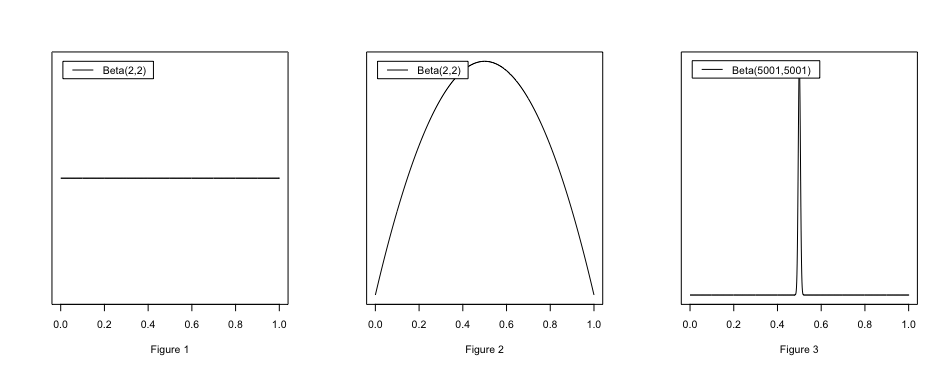
\includegraphics{beta.png}
\caption{Beta Distributions}
\end{figure}

Intuitively, we can think of the first distribution as representing your
state of belief about the probability of getting a head on the next
flip. This distribution is plotted in Figure 1: note that it is wholly
flat, capturing the sort of state of indifference that the Principle of
Indifference is supposed to capture: One finds no ground in thinking one
probability is more credible than another.

The second distribution can be seen as our state of belief after
witnessing 10 flips of the coin, and 5 turn up heads and 5 tails.
Naturally, the peak - the mode of the distribution - is at
\(\theta = 0.5\), which seems sensible, because it reflects the evidence
that exactly half of the samples are heads. But we can see that at this
stage we are quite uncertain about \(\theta\), evidenced by the width of
the distribution. While \(\theta = 0.5\) is the peak, there is a
substantial area covering \(\theta > 0.55\) and \(\theta < 0.45\).

The third distribution, modeling the state of belief after one million
trials with half of them being heads, is intended to be an approximation
of Popper's ideal evidence scenario. The peak is again at \(0.5\), but
this plot has a noticeably narrower spread: we are much more confident
in our assessment that the coin has an equal propensity to land on heads
as tails. Also notice that at this stage, any value of \(\theta\) other
than \(0.5\) are practically impossible after receiving the ideal
evidence.

To state these observations more precisely, we can calculate the exact
probability using the corresponding cumulative distributions. Since beta
distributions are continuous distributions, we can only deal with
intervals of values. Still, we can provide a reasonably close
approximations. For instance, conditional on the ideal evidence, we
would be absolutely sure that the probability is between 0.46 and 0.54,
and practically certain, with the probability of 0.95, that it is
between 0.49 and 0.51. The relevant probabilities are summarized in the
following table:

\begin{longtable}[]{@{}lrr@{}}
\toprule
Distribution & \(P(0.46<\theta<0.54)\) &
\(P(0.49<\theta<0.51)\)\tabularnewline
\midrule
\endhead
\(Beta(1,1)\) & \(0.08\) & \(0.02\)\tabularnewline
\(Beta(11,11)\) & \(0.29\) & \(0.07\)\tabularnewline
\(Beta(500001,500001)\) & \(1\) & \(1\)\tabularnewline
\bottomrule
\end{longtable}

Now, let \(E\) be the ideal evidence, \(X_1,…X_{1000000}\), where
\(\sum_{i=1}^{1000000}X_i = 500000\), and let \(\theta\) be the coin's
propensity to land on heads. We now see that the following inequality
holds, since the left-hand side is \(0.02\), and for the right it's
\(1\).

\[P(0.49<\theta<0.51) <  P(0.49<\theta<0.51|E)\]

To make things more official-sounding, perhaps we can describe this as
\emph{Higher Order Relevance(HOR)}. Recall Keynes's idea is that for
some evidence \(E\) and hypothesis \(H\)

\[\text{Evidence $E$ is relevant to $H$ if and only if }P(H) \neq P(H|E)\]

HOR takes this on step further and suggests that, in addition to \(H\)
and \(E\), consider specific values \(x\) and \(y\), where
\(0 \leq x \leq y \leq 1\)

\[\text{Evidence $E$ has a higher order relevance to $x\leq \theta \leq y)$ iff}\]
\[P(x\leq \theta \leq y) \neq P(x\leq \theta \leq y)|E)\]

Under this analysis, we can see that Popper's argument contains a
sleight of hand that shifts between two ways of thinking about N---the
next coin toss landing on heads---'s probability. The argument begins by
asking, rather innocuously, for your prior for \(N\), but the ideal
evidence \(I\) Popper immediately introduced is not for \(N\) but for
the hypothesis that \(\theta = 0.5\). Popper is reasonably explicit
about \emph{that}, but what he is not explicit about is \emph{this}: he
has convinced us that \(I\) is both evidentially ideal for and
conditionally relevant to \(\theta = 0.5\). That, however, is a
misdirection, because he immediately starts talking the conditional
probability on \(I\), \emph{not} of \(H_{0.5}\), but of \(N\).

While I think that HOR provides a sufficient response to Popper's
paradox, it is not quite the same as accounting for the phenomenon in
question. In fact, by focusing on overcoming the difficulty raised by
the paradox caused by an absurd amount of evidence, we might have
overlooked what is truly at stake: rarely, if ever, do we have ideal
evidence for any substantive hypothesis, so situations where we have an
overabundance of evidence is an incomplete benchmark for the adequacy of
the account. In fact, our analysis shows that when we have perfect
information, evidential weight essentially becomes a non-issue, because
it eliminates the uncertainty that calls for probabilistic reasoning to
begin with.

The important question, instead, is whether HOR can help with decision
making in situations where evidence is severely lacking. To this end, it
remains to be seen how higher order relevance can trickle down to first
order probability, on which decision making is based within the
classical Bayesian framework.

We need to, then, ask ourselves if HOR as a concept can make any
practical difference in decision making. It is in fact difficult to do
so within the basic framework of Bayesianism. To see this, imagine a
perverse game in which you will be shot to death if a coin flip lands on
head. Clearly, you don't want heads. You are given a choice between two
coins: the first coin \(P\) is similar to Popper's coin from the ideal
evidence scenario, except now the ideal evidence actually shows that
there is a slight bias in favor of heads, say the expected value is
0.51. The other coin \(U\) is one you have never seen before, so on an
ignorance prior your expected value \(E(\theta_U)\) is 0.5 . Now, which
would you choose? An argument can be made that you probably still want
the Popperian coin, because you know you are almost certainly getting
\(\theta_P = 0.51\). From the perspective of expected utility, however,
it is hard to rationalize such a decision, because the unknown coin
still has a lower expected value. That is,

\[\frac{510000}{1000000}> \frac{1}{2}\]

So it seems that we are back to where we started - the relevance
demonstrated on a higher order simply vanishes when we consider the
matter on the level of decision making, which is entirely based on a
precise point-estimate of the first order probability.

If the point estimate is to be blamed, the natural response is that we
do rely on an interval estimate instead. This solution is reminiscent of
the call to abolish the use of \(p\) values in Frequentist statistics,
and instead we should report the confidence interval of our findings.
The idea is that point estimates are inherently misleading, since they,
by design, summarize the data by discarding information such as higher
order relevance. This problem is somewhat analogous to the one we are
running into with respect to expected values. So one possible solution
is that we should only insist on making our decisions based on
\emph{credible intervals}, which is the Bayesian version of the
confidence interval. For instance, suppose
\(\theta_P \sim Beta(480000,520000)\) and \(\theta_U \sim Beta(1,1)\).
We can deduce that

\[P(0.479\leq \theta_P \leq 0.481) = 0.99\]
\[P(0.005\leq \theta_U \leq 0.995) = 0.99\]

\noindent In other words, we can say there is a 0.99 probability that
\(P\)'s propensity to land on heads is between 0.479 and 0.481
(practically 0.48) and for \(U\) it's between 0.005 and 0.995.

However, it seems to me that we are simply restating higher order
relevance in terms of credible intervals, without dealing with the crux
of the problem - unless we are rationally allowed to refuse to follow
the precise expected value, even if the weight of evidence is low, we
will always have to match it to our best point estimate, which is the
expected value. Of course, the point is not that HOR doesn't matter,
because intuitively it does. The point is rather that we need a richer
philosophical framework to rationalize this intuition.

\hypertarget{the-concept-of-resiliency-1}{%
\subsection{The Concept of
Resiliency}\label{the-concept-of-resiliency-1}}

Skyrms credits Richard Jeffrey as the first who notices that Popper's
paradox brings light to the very idea of resiliency. Jeffrey points out
that once we stop fixating on the probability of \(N\), the next toss
coming up head, we can see that our state of belief prior receiving the
ideal evidence has a degree of malleability.\footnote{Jeffrey,
  \emph{Logic of Decision}, 184.} Consider, for instance, instead of
asking only for the probability of \(N\), we ask the probability of the
next 5 tosses coming up heads. Once we think about how our belief
responds to how these 5 tosses would act as potential evidence, given
our posterior state of belief, we have very little choice but to believe
that probability is \((0.5)^5\), but we would be a lot less compelled to
do so with the prior state of belief.

Skyrms has proposed the notion of \emph{resiliency} to capture Jeffrey's
observation in a generalized manner: even though evidential weight is
not reflected by the probability, it is captured by its stability. The
idea that there is a probabilistic representation for a stable state of
belief can be illustrated as follows: if I have in front of me an urn
\(U\), with an unknown proportion of black and white balls. If I
randomly draw 2 balls from it with replacement and find one ball for
each color, my intuitive estimate of the proportion of black balls would
sensibly be somewhere around 1/2. But my state of belief should be
relatively unstable: it would be irrational for me to fixate on this
estimate, especially new light of conflicting evidence. If I sample two
more balls from the urn and they are both black, it would make sense for
me to raise my estimate for the proportion of black balls to more than
1/2---perhaps to 3/4. But suppose I continue to sample from for 996 more
times. Out of the total 1000 draws, 500 are black. At this point a
sensible would be back to around 1/2, but unlike my state of belief
after only 2 samples, after 1000 samples my state of belief is
stabilized: suppose I sample again and I draw five black balls in a row.
Now, even though drawing 5 black balls in a row seems rather
extraordinary, against the body of my evidence it would not warrant me
to revise my belief in any significant measure.

The intuition here is that the increase in the amount of evidence,
expressed here in terms of the number of samples, corresponds to the
increase of stability of the estimate. Skyrms has introduced a notion
called the \emph{resiliency} to capture this intuition sense of
stability.

Conceptually, this is an attractive way to capture to notion of
evidential weight. Keynes' puzzlement about how relevance and weight
could come apart is addressed; When a belief \(B\) is resilient, the
conditional probability on some new evidence \(E\) should be
approximately the same, that is, \(P(B|E) \approx P(B)\), even if \(E\)
would be highly relevant were \(B\) not resilient. If, for instance, a
resilient belief is one where the weight of the evidence for it is high,
then it is a logical consequence that evidence could make a belief more
weighty without changing its degree, for the weight is in fact
stabilizing this particular value.

Nevertheless, how the resilience of a belief can make a practical
difference is yet to be explained. In fact, for the most part,
resiliency does not do much better than higher order relevance: within
the structure of expected utility calculus, a highly resilient belief
will still recommend the same action as a non-resilient belief with the
same expected value. Skyrms' original motivation for the concept,
however, provides an important clue: he intended the concept of
resiliency to explicate the concept of the laws of nature, so the idea
is that a probability statement \(A\) based on a law of nature is one
that remains resilient against various extreme scenarios. What this
means is that we are supposed to calculate likelihoods based on data
that \emph{might have happened}, and see whether \(A\) is resilient
against it.

\hypertarget{counterfactual-priors-and-hypothetical-data-1}{%
\subsection{Counterfactual Priors and Hypothetical
Data}\label{counterfactual-priors-and-hypothetical-data-1}}

The notion of resiliency opens the door to how counterfactual reasoning
can be relevant in Bayesian reasoning. The crucial point is that to see
how resilient a probability is, it is not something we can determine by
looking at data that we already have. We have examine what \emph{might
have happened}. So notwithstanding Lindley's rhetorical question:

\begin{quote}
Of what relevance are things that might have happened, but did
not?\footnote{Lindley and Phillips, ``Inference for a Bernoulli Process
  (a Bayesian View),'' 114.}
\end{quote}

Counterfactual considerations are relevant in deliberating on how a
chosen hypothesis \emph{would} respond in light of confounding
scenarios, so that we can decide if it is a worthy hypothesis and, if
chosen, how we ought to further probe it. More specifically, the weight
of evidence is puzzling, because it needs to be understood in the
context of abduction, since its goal is to give information about how we
ought to structure our inductive space.

Skyrms suggests that the resilience of a belief manifests itself as ``a
reluctance to change.''\footnote{Skyrms, ``Resiliency, Propensities, and
  Causal Necessity,'' 707.} He suggests that we can measure weight
directly in terms of the difference between prior and posterior
probabilities. Perhaps we can call this the measure of instability,
which signifies a lack of weight:

\[\text{Instability: }|P(X|E_j) - y|\]

Where \(j\) is in the set of \(n\) possible states of affairs,
\(E_1,..., E_n\). Skyrms' idea is that we should pick a \(j\) that
creates the biggest difference.

To see what this means, consider how resiliency can be demonstrated
using the beta distribution, though keep in mind that it is not meant to
be a generalizable result, since different distributions work
differently. In any case, recall that different sets of parameters can
produce the same expected value. For instance, consider \(Beta(1,1)\)
and \(Beta(5000,5000)\). Their expected values are, of course, the same,
since \(\frac{1}{2} = \frac{5000}{10000}\). But the second distribution
is way much resilient than the first. Suppose these are distribution
functions that represent the opinions of two different agents, but they
both receive the same piece of evidence \(Y\) from a Bernoulli process
such that \(Y=\sum_{i=1}^5 X_i=5\), that is, getting 5 heads in a row.
We do not have to do the calculation to see that they will respond to
the evidence pretty differently: the first agent will raise her
posterior expected value from \(1/2\) to \(6/7\). The difference is
\(.36\), which is a considerable increase.

The second agent's opinion, however, would barely be changed:

\[\frac{5005}{10005} - \frac{5000}{10000} = 0.00025\]

It is barely a rounding error. In fact, we can see that the second agent
would have to see 200 successes \emph{in a row} in order to raise the
credence by \(0.01\):

\[\frac{5000+200}{5000+5000+200} = 0.51\]

Notice that this analysis requires counterfactual thinking in two ways:
we have to consider what our priors \emph{would} be like in different
circumstances, and we have to consider its response to some hypothetical
data. This is why the weight of evidence is a dispositional commitment:
one is committed to respond to the the deliverance of experience in a
deliberate manner, as dictated by the model decided upon after
considering various counterfactual scenarios.

This way of understanding evidential weight provides an important
insight on the voluntaristic idea that degrees of belief ought to be
understood as taking up an epistemic commitment during the context of
abduction. To deliberate on the appropriate hypothesis to be accepted
provisionally, I have to know what \emph{practical difference} its
acceptance would make on my future conduct. To do so, I have to draw
deductive inferences based on various possible models that I could
possibly accept, based on various hypothetical scenarios that come up
during experiment.

To see what I mean, it might help to see the interaction between the
evidence and posterior probability directly---this is shown in the
figure. The x-axis represents the number of heads in a row, so the
higher x is, the more extreme the hypothetical evidence is. The y-axis
is the posterior probability after receiving the x heads out of x throws
as indicated by the x-axis.

\begin{figure}
\centering
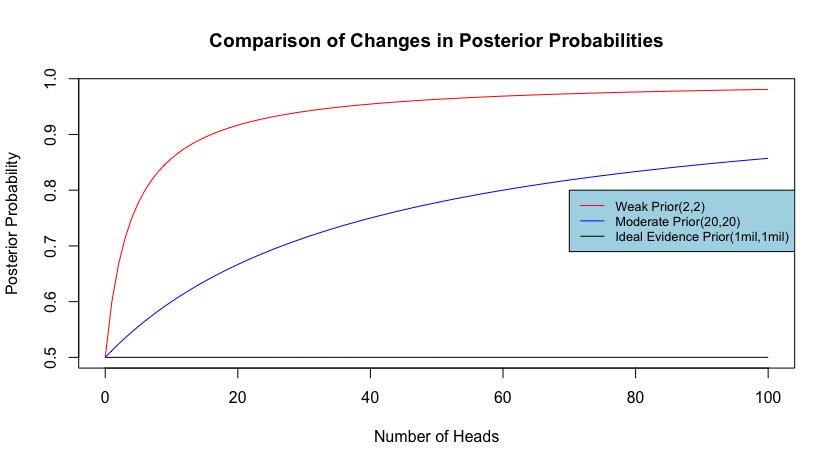
\includegraphics{rescompare.png}
\caption{Comparison of stabilities of different prior distributions:
values in parentheses are parameters for the beta distribution.}
\end{figure}

We see that these counterfactual priors behave quite differently in
slight of extreme evidence. Here, the weight of evidence clearly
corresponds to the sum of the parameters \(\alpha + \beta\), and the
higher it is, the less responsive it is to evidence. This is especially
clear when \(\alpha = \beta = 500\)---we see that with such as a weighty
prior distribution, it makes absolutely no difference how the extreme
the data is, until we get more than 60 heads in a row. Even if we tossed
100 out of 100, the expected value stays very close to \(0.5\). A ``flat
prior'', i.e., \(\alpha = \beta = 1\), is, as expected, not resilient
against almost any form of extreme evidence. The posterior is expected
to almost \(0.8\) after seeing 10 heads in a row, and rapidly approaches
unity.

From the deliberativist point of view, there is no \emph{a priori}
justification for one over another. There are circumstances in which the
extremely recalcitrant prior would be appropriate. Perhaps we can
consider the probability of a person's guilt based on the evidence. In
such a case, it would be rational to adopt a prior that is extremely
resilient, so that the posterior would be unresponsive unless the
evidence is beyond any reasonable doubt. Even in a less dramatic
situation such as testing the effectiveness of a drug, a resilient prior
could still be advisable when the result could mean have life-altering
consequences.

This also has an implication on the voluntarist interpretation of
degrees of belief. Recall that van Fraassen argues that assertions of
probability should not be a description of the agent's psychological
state. An argument for the voluntarist reading can be made in this
context. Suppose personally I think the coin is extremely likely to be
fair. It seems \emph{less} rational for me to adopt a prior to reflect
such a state, e.g., \(Beta(500,500)\); because, it would look as though
I am rigging the experiment in favor of \emph{my} hypothesis. The
rational thing, as a matter of fact, should be the opposite:
\emph{because} I am confident that my opinion is true, I am
intentionally adopting the opposite prior, with the assumption that the
data will overwhelm it. This is akin to a gambler with inside
information who is willing to make a bet with extremely unfavorable
odds. As the psychologist John Kruschke points out, it might be
advisable to choose a prior to satisfy a skeptic.\footnote{Kruschke,
  ``Bayesian Estimation Supersedes the T Test,'' 575.}

\hypertarget{refs}{}
\leavevmode\hypertarget{ref-austin}{}%
Austin, J. L. \emph{How to Do Things with Words}. Clarendon Press, 1962.

\leavevmode\hypertarget{ref-ayerpae}{}%
Ayer, A. J. \emph{Probability and Evidence}. Macmillan, 1972.

\leavevmode\hypertarget{ref-robust}{}%
Berger, James. ``The Robust Bayesian Viewpoint.'' In \emph{Robustness of
Bayesian Analyses}, edited by J. D. Kadane. Elsevier Science, 1984.

\leavevmode\hypertarget{ref-whatpragwas}{}%
Burke, F. Thomas. \emph{What Pragmatism Was}. Indiana University Press,
2013.

\leavevmode\hypertarget{ref-carnapprob}{}%
Carnap, Rudolf. \emph{Logical Foundations of Probability}.
Chicago{]}University of Chicago Press, 1950.

\leavevmode\hypertarget{ref-logicalsyntax}{}%
---------. \emph{The Logical Syntax of Language}. London: K. Paul,
Trench, Trubner \& Co., 1937.

\leavevmode\hypertarget{ref-cleverbookies}{}%
Christensen, David. ``Clever Bookies and Coherent Beliefs.''
\emph{Philosophical Review} 100, no. 2 (1991): 229--47.

\leavevmode\hypertarget{ref-med}{}%
Descartes, René. \emph{The Philosophical Writings of Descartes}. Vol. 1.
Cambridge University Press, 1984.

\leavevmode\hypertarget{ref-elgadisagreement}{}%
Elga, Adam. ``Reflection and Disagreement.'' \emph{Noûs} 41, no. 3
(2006): 478--502.

\leavevmode\hypertarget{ref-ellsberg}{}%
Ellsberg, Daniel. ``Risk, Ambiguity, and the Savage Axioms.'' \emph{The
Quarterly Journal of Economics} 75, no. 4 (1961): 643--69.

\leavevmode\hypertarget{ref-definepis}{}%
Finetti, Bruno de. \emph{Probability, Induction, and Statistics}. Wiley,
1972.

\leavevmode\hypertarget{ref-beliefwill}{}%
Fraassen, Bas C. Van. ``Belief and the Will.'' \emph{Journal of
Philosophy} 81, no. 5 (1984): 235--56.

\leavevmode\hypertarget{ref-beliefuly}{}%
Fraassen Bas C. ``Belief and the Problem of Ulysses and the Sirens.''
\emph{Philosophical Studies} 77, no. 1 (1995): 7--37.

\leavevmode\hypertarget{ref-bvflaws}{}%
Fraassen, Bas C. van. \emph{Laws and Symmetry}. Oxford University Press,
1989.

\leavevmode\hypertarget{ref-gelman}{}%
Gelman, Andrew, and Cosma Rohilla Shalizi. ``Philosophy and the Practice
of Bayesian Statistics in the Social Sciences.'' In \emph{The Oxford
Handbook of Philosophy of Social Science}, edited by Harold Kincaid.
Oxford University Press, 2012.

\leavevmode\hypertarget{ref-goodtotalevidence}{}%
Good, I. J. ``On the Principle of Total Evidence.'' \emph{British
Journal for the Philosophy of Science} 17, no. 4 (1966): 319--21.

\leavevmode\hypertarget{ref-goodthinking}{}%
Good, Irving J. \emph{Good Thinking: The Foundations of Probability and
Its Applications}. Univ Minnesota Pr, 1983.

\leavevmode\hypertarget{ref-goodmancounterfactual}{}%
Goodman, Nelson. ``The Problem of Counterfactual Conditionals.''
\emph{Journal of Philosophy} 44, no. 5 (1947): 113--28.

\leavevmode\hypertarget{ref-forgetful}{}%
Greenwald, David. ``The Forgetful Witness.'' \emph{The University of
Chicago Law Review} 160, no. 1 (1993): 167--95.

\leavevmode\hypertarget{ref-hajekdutchbook}{}%
Hajek, Alan. ``Dutch Book Arguments.'' In \emph{The Oxford Handbook of
Rational and Social Choice}, edited by Paul Anand, Prasanta Pattanaik,
and Clemens Puppe. Oxford University Press, 2008.

\leavevmode\hypertarget{ref-hookway1}{}%
Hookway, Christopher. \emph{Truth, Rationality, and Pragmatism: Themes
from Peirce}. Oxford University Press, 2000.

\leavevmode\hypertarget{ref-hoover1994}{}%
Hoover, Kevin. ``Pragmatism, Pragmaticism, and Economic Method.'' In
\emph{New Directions in Economic Methodology}. Routledge, 1994.

\leavevmode\hypertarget{ref-jameswill}{}%
James, William. \emph{The Will to Believe and Human Immortality}. Dover
Publications, 1960.

\leavevmode\hypertarget{ref-jeffreydecision}{}%
Jeffrey, Richard. \emph{Logic of Decision}. McGraw-Hill, 1965.

\leavevmode\hypertarget{ref-joycenonprag}{}%
Joyce, James M. ``A Nonpragmatic Vindication of Probabilism.''
\emph{Philosophy of Science} 65, no. 4 (1998): 575--603.

\leavevmode\hypertarget{ref-prospect}{}%
Kahneman, Daniel, and Amos Tversky. ``Prospect Theory: An Analysis of
Decision Under Risk.'' \emph{Econometrica: Journal of the Econometric
Society}, 1979, 263--91.

\leavevmode\hypertarget{ref-keynes}{}%
Keynes, John Maynard. \emph{A Treatise on Probability}. Macmillan; Co.,
Limited., 1921.

\leavevmode\hypertarget{ref-keynesbio}{}%
---------. \emph{Essays in Biography}. Macmillan; Co., Limited., 1933.

\leavevmode\hypertarget{ref-kruschkettest}{}%
Kruschke, John K. ``Bayesian Estimation Supersedes the T Test.''
\emph{Journal of Experimental Psychology: General} 142, no. 2 (2013):
573.

\leavevmode\hypertarget{ref-laplace}{}%
Laplace, Pierre-Simon. \emph{Philosophical Essay on Probabilities}.
Spring, 1995.

\leavevmode\hypertarget{ref-levibeware}{}%
Levi, Isaac. ``11 Beware of Syllogism: Statistical Reasoning and
Conjecturing According to Peirce.'' In \emph{The Cambridge Companion to
Peirce}, edited by C. J. Misak, 257. Cambridge University Press, 2004.

\leavevmode\hypertarget{ref-leviweight}{}%
---------. ``The Weight of Argument.'' In \emph{Fundamental Uncertainty:
Rationality and Plausible Reasoning}, edited by Silva Marzetti Dall'Aste
Brandolini and Roberto Sczzieri, 39--58. Palgrave MacMilan, 2011.

\leavevmode\hypertarget{ref-lewisguide}{}%
Lewis, David. ``A Subjectivist's Guide to Objective Chance.'' In
\emph{Philosophy of Probability: Contemporary Readings}, edited by
Richard C. Jeffrey, 183--98. University of California Press, 1980.

\leavevmode\hypertarget{ref-lindleybern}{}%
Lindley, D. V., and L. D. Phillips. ``Inference for a Bernoulli Process
(a Bayesian View).'' \emph{The American Statistician} 30, no. 3 (1976):
112--19.

\leavevmode\hypertarget{ref-lipton}{}%
Lipton, Peter. \emph{Inference to the Best Explanation}.
Routledge/Taylor; Francis Group, 2004.

\leavevmode\hypertarget{ref-errorstat}{}%
Mayo, Deborah G., and Aris Spanos. ``Error Statistics.'' In
\emph{Handbook of the Philosophy of Science, Vol. 7: Philosophy of
Statistics}, edited by Prasanta S. Bandyopadhyay and Malcolm R. Forster.
Elsevier B.V., 2011.

\leavevmode\hypertarget{ref-pascal}{}%
``Pascal's Pensées.''
\url{https://www.gutenberg.org/files/18269/18269-h/18269-h.htm}, n.d.

\leavevmode\hypertarget{ref-probableinference}{}%
Peirce, Charles S. ``A Theory of Probable Inference.'' In \emph{Writings
of Charles S. Peirce: A Chronological Edition, Volume 4: 1879--1884}.
Indiana University Press, 1989.

\leavevmode\hypertarget{ref-CP}{}%
---------. \emph{Collected Papers of Charles Sanders Peirce}. Cambridge:
Harvard University Press, 1931.

\leavevmode\hypertarget{ref-makeideasclear}{}%
---------. ``How to Make Our Ideas Clear.'' In \emph{Writings of Charles
S. Peirce: A Chronological Edition, Volume 3: 1872--1878}. Indiana
University Press, 1966.

\leavevmode\hypertarget{ref-essentialpeirce2}{}%
---------. \emph{The Essential Peirce, Volume 2: Selected Philosophical
Writings (1893-1913)}. Edited by Peirce Edition Project. Indiana
University Press, 1998.

\leavevmode\hypertarget{ref-probabilityofinduction}{}%
---------. ``The Probability of Induction.'' In \emph{Writings of
Charles S. Peirce: A Chronological Edition, Volume 3: 1872--1878}.
Indiana University Press, 1986.

\leavevmode\hypertarget{ref-popperlogic}{}%
Popper, Karl. \emph{The Logic of Scientific Discovery}. Routledge, 2002.

\leavevmode\hypertarget{ref-epistnat}{}%
Quine, W. V. ``Epistemology Naturalized.'' In \emph{Ontological
Relativity and Other Essays}. New York: Columbia University Press, 1969.

\leavevmode\hypertarget{ref-quinefromstim}{}%
---------. \emph{From Stimulus to Science}. Harvard University Press,
1997.

\leavevmode\hypertarget{ref-appliedstatdec}{}%
Raiffa, Howard, and Robert Schlaifer. \emph{Applied Statistical Decision
Theory}. Harvard, 1964.

\leavevmode\hypertarget{ref-ramseyvalue}{}%
Ramsey, F. P. ``Weight or the Value of Knowledge.'' \emph{British
Journal for the Philosophy of Science} 41, no. 1 (1990): 1--4.

\leavevmode\hypertarget{ref-ramsey}{}%
Ramsey, Frank P. \emph{Philosophical Papers}. Cambridge: Harvard
University Press, 1990.

\leavevmode\hypertarget{ref-greenmoore}{}%
S., Green Mitchell, and Williams John N. \emph{Moore's Paradox: New
Essays on Belief, Rationality, and the First Person}. Oxford University
Press, 2007.

\leavevmode\hypertarget{ref-savage}{}%
Savage, Leonard J. \emph{The Foundations of Statistics}. Dover, 1954.

\leavevmode\hypertarget{ref-searle}{}%
Searle, John R. \emph{Speech Acts: An Essay in the Philosophy of
Language}. Cambridge University Press, 1969.

\leavevmode\hypertarget{ref-shackles}{}%
Shackles, G.L.S. \emph{Uncertainty in Economics and Other Reflections}.
Cambridge University Press, 1955.

\leavevmode\hypertarget{ref-causationandconditional}{}%
Skyrms, Brain. ``Resiliency, Propensities, and Causal Necessity.''
\emph{Journal of Philosophy} 74, no. 11 (1966): 704--13.

\leavevmode\hypertarget{ref-twoprinciplesofbayesian}{}%
Talbott, William. ``Two Principles of Bayesian Epistemology.''
\emph{Philosophical Studies} 62, no. 2 (1991): 135--50.

\leavevmode\hypertarget{ref-walley}{}%
Walley, Peter. \emph{Statistical Reasoning with Imprecise
Probabilities}. Chapman \& Hall, 1991.

\leavevmode\hypertarget{ref-winkler}{}%
Winkler, Robert. \emph{An Introduction to Bayesian Inference and
Decision}. Probabilistic Publishing, 2010.

\end{document}
